% Options for packages loaded elsewhere
\PassOptionsToPackage{unicode}{hyperref}
\PassOptionsToPackage{hyphens}{url}
%
\documentclass[
]{book}
\usepackage{amsmath,amssymb}
\usepackage{iftex}
\ifPDFTeX
  \usepackage[T1]{fontenc}
  \usepackage[utf8]{inputenc}
  \usepackage{textcomp} % provide euro and other symbols
\else % if luatex or xetex
  \usepackage{unicode-math} % this also loads fontspec
  \defaultfontfeatures{Scale=MatchLowercase}
  \defaultfontfeatures[\rmfamily]{Ligatures=TeX,Scale=1}
\fi
\usepackage{lmodern}
\ifPDFTeX\else
  % xetex/luatex font selection
\fi
% Use upquote if available, for straight quotes in verbatim environments
\IfFileExists{upquote.sty}{\usepackage{upquote}}{}
\IfFileExists{microtype.sty}{% use microtype if available
  \usepackage[]{microtype}
  \UseMicrotypeSet[protrusion]{basicmath} % disable protrusion for tt fonts
}{}
\makeatletter
\@ifundefined{KOMAClassName}{% if non-KOMA class
  \IfFileExists{parskip.sty}{%
    \usepackage{parskip}
  }{% else
    \setlength{\parindent}{0pt}
    \setlength{\parskip}{6pt plus 2pt minus 1pt}}
}{% if KOMA class
  \KOMAoptions{parskip=half}}
\makeatother
\usepackage{xcolor}
\usepackage{longtable,booktabs,array}
\usepackage{calc} % for calculating minipage widths
% Correct order of tables after \paragraph or \subparagraph
\usepackage{etoolbox}
\makeatletter
\patchcmd\longtable{\par}{\if@noskipsec\mbox{}\fi\par}{}{}
\makeatother
% Allow footnotes in longtable head/foot
\IfFileExists{footnotehyper.sty}{\usepackage{footnotehyper}}{\usepackage{footnote}}
\makesavenoteenv{longtable}
\usepackage{graphicx}
\makeatletter
\def\maxwidth{\ifdim\Gin@nat@width>\linewidth\linewidth\else\Gin@nat@width\fi}
\def\maxheight{\ifdim\Gin@nat@height>\textheight\textheight\else\Gin@nat@height\fi}
\makeatother
% Scale images if necessary, so that they will not overflow the page
% margins by default, and it is still possible to overwrite the defaults
% using explicit options in \includegraphics[width, height, ...]{}
\setkeys{Gin}{width=\maxwidth,height=\maxheight,keepaspectratio}
% Set default figure placement to htbp
\makeatletter
\def\fps@figure{htbp}
\makeatother
\setlength{\emergencystretch}{3em} % prevent overfull lines
\providecommand{\tightlist}{%
  \setlength{\itemsep}{0pt}\setlength{\parskip}{0pt}}
\setcounter{secnumdepth}{5}
\usepackage{booktabs}
\ifLuaTeX
  \usepackage{selnolig}  % disable illegal ligatures
\fi
\usepackage[]{natbib}
\bibliographystyle{plainnat}
\usepackage{bookmark}
\IfFileExists{xurl.sty}{\usepackage{xurl}}{} % add URL line breaks if available
\urlstyle{same}
\hypersetup{
  pdftitle={GTI - Governança da Informação - 2025 - Anotações de aula},
  pdfauthor={Professor Miguél Suares},
  hidelinks,
  pdfcreator={LaTeX via pandoc}}

\title{GTI - Governança da Informação - 2025 - Anotações de aula}
\author{Professor Miguél Suares}
\date{2025-08-31}

\begin{document}
\maketitle

{
\setcounter{tocdepth}{1}
\tableofcontents
}
\chapter*{Sobre estas anotações}\label{sobre-estas-anotauxe7uxf5es}
\addcontentsline{toc}{chapter}{Sobre estas anotações}

---------------------------------------------------------------------------------------------------------------------------------------

Estas anotações são apenas lembretes das aulas expostas em sala, durante a disciplina de Governança da Informação.

\section{ACESSO AO GITBOOK CELULAR}\label{acesso-ao-gitbook-celular}

---------------------------------------------------------------------------------------------------------------------------------------

\subsubsection{\texorpdfstring{\url{https://miguel7penteado.github.io/2025-2sem-GTI-Governanca}}{https://miguel7penteado.github.io/2025-2sem-GTI-Governanca}}\label{httpsmiguel7penteado.github.io2025-2sem-gti-governanca}


\includegraphics{images/qr-code-disciplina.jpg}

\section{Leitores de formato de arquivo EPUB para SmartPhone}\label{leitores-de-formato-de-arquivo-epub-para-smartphone}

---------------------------------------------------------------------------------------------------------------------------------------

\subsection{ANDROID}\label{android}

\subsubsection{\texorpdfstring{\textbf{Moon+ Reader}}{Moon+ Reader}}\label{moon-reader}


\includegraphics[width=3.54167in,height=\textheight]{images/qrcode/leitor_epub/MoonReaderPlus.jpg}

\section{Livros Texto da Disciplina}\label{livros-texto-da-disciplina}

---------------------------------------------------------------------------------------------------------------------------------------

\subsection{\texorpdfstring{``Governança Corporativa'' dos autores ``\textbf{José Paschoal Rossetti e Adriana Andrade}''}{``Governança Corporativa'' dos autores ``José Paschoal Rossetti e Adriana Andrade''}}\label{governanuxe7a-corporativa-dos-autores-josuxe9-paschoal-rossetti-e-adriana-andrade}


\includegraphics{images/livros/livro1.jpg}

\begin{longtable}[]{@{}
  >{\raggedright\arraybackslash}p{(\columnwidth - 2\tabcolsep) * \real{0.1620}}
  >{\raggedright\arraybackslash}p{(\columnwidth - 2\tabcolsep) * \real{0.8380}}@{}}
\toprule\noalign{}
\endhead
\bottomrule\noalign{}
\endlastfoot
\textbf{Autor(es)} & \href{https://www.fdc.org.br/sobreafdc/professores/rossetti}{\textbf{José Paschoal Rossetti}} \textbf{e \href{https://tradeconbusiness.com.br/nossa-equipe/adriana-de-andrade-sole/}{Adriana Andrade}} \\
\textbf{Editora} & Atlas \\
\textbf{Idioma} & Português \\
\textbf{ISBN} & 9788522493050 \\
\textbf{Formato} & Capa dura \\
\textbf{Páginas} & 608 \\
\textbf{Código Biblioteca} & \\
\end{longtable}

\subsection{``Implantando a Governança de TI (4ª edição): Da estratégia à gestão de processos e serviços'' dos autores ``Aguinaldo Aragon Fernandes e Vladimir Ferraz de Abreu''}\label{implantando-a-governanuxe7a-de-ti-4uxaa-ediuxe7uxe3o-da-estratuxe9gia-uxe0-gestuxe3o-de-processos-e-serviuxe7os-dos-autores-aguinaldo-aragon-fernandes-e-vladimir-ferraz-de-abreu}

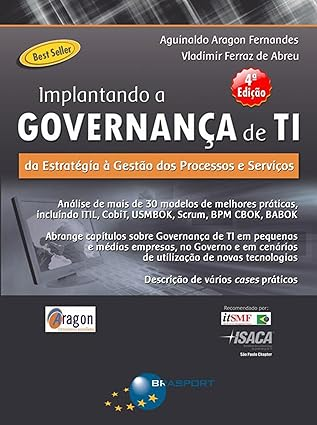
\includegraphics{images/livros/livro2.jpg}

\begin{longtable}[]{@{}
  >{\raggedright\arraybackslash}p{(\columnwidth - 2\tabcolsep) * \real{0.1290}}
  >{\raggedright\arraybackslash}p{(\columnwidth - 2\tabcolsep) * \real{0.8710}}@{}}
\toprule\noalign{}
\endhead
\bottomrule\noalign{}
\endlastfoot
\textbf{Autor(es)} & \begin{minipage}[t]{\linewidth}\raggedright
\subsubsection{\texorpdfstring{\href{https://br.linkedin.com/in/aguinaldo-aragon-fernandes}{Aguinaldo Aragon Fernandes} e \href{https://br.linkedin.com/in/vladimirabreu}{Vladimir Ferraz de Abreu}}{Aguinaldo Aragon Fernandes e Vladimir Ferraz de Abreu}}\label{aguinaldo-aragon-fernandes-e-vladimir-ferraz-de-abreu}
\end{minipage} \\
\textbf{Editora} & BRASPORT \\
\textbf{Idioma} & Português \\
\textbf{ISBN-13} & 978-8574528441 \\
\textbf{Formato} & Eletrônico \\
\textbf{Páginas} & 1198 \\
\textbf{Código Biblioteca} & \\
\end{longtable}

\section{Calendário das aulas}\label{calenduxe1rio-das-aulas}

---------------------------------------------------------------------------------------------------------------------------------------

\paragraph{AGOSTO DE 2025}\label{agosto-de-2025}

\begin{longtable}[]{@{}llll@{}}
\toprule\noalign{}
Data & Dia da Semana & Aulas & Conteúdo \\
\midrule\noalign{}
\endhead
\bottomrule\noalign{}
\endlastfoot
06/08/2025 & Quarta-Feira & Aula Inaugural & \\
13/08/2025 & Quarta-Feira & Aula 2 & \\
20/08/2025 & Quarta-Feira & Aula 3 & \\
27/08/2025 & Quarta-Feira & Aula 4 & \\
\end{longtable}

\paragraph{SETEMBRO DE 2025}\label{setembro-de-2025}

\begin{longtable}[]{@{}llll@{}}
\toprule\noalign{}
Data & Dia da Semana & Aulas & Conteúdo \\
\midrule\noalign{}
\endhead
\bottomrule\noalign{}
\endlastfoot
03/09/2025 & Quarta-Feira & Aula 5 & \\
10/09/2025 & Quarta-Feira & Aula 6 & \\
17/09/2025 & Quarta-Feira & NP1 & PROVA \\
24/09/2025 & Quarta-Feira & Aula 7 & \\
\end{longtable}

\paragraph{OUTUBRO DE 2025}\label{outubro-de-2025}

\begin{longtable}[]{@{}llll@{}}
\toprule\noalign{}
Data & Dia da Semana & Aulas & Conteúdo \\
\midrule\noalign{}
\endhead
\bottomrule\noalign{}
\endlastfoot
01/10/2025 & Quarta-Feira & Aula 8 & \\
08/10/2025 & Quarta-Feira & Aula 9 & \\
15/10/2025 & Quarta-Feira & Aula 10 & \\
22/10/2025 & Quarta-Feira & Aula 11 & \\
29/10/2025 & Quarta-Feira & Aula 12 & \\
\end{longtable}

\paragraph{NOVEMBRO DE 2025}\label{novembro-de-2025}

\begin{longtable}[]{@{}llll@{}}
\toprule\noalign{}
Data & Dia da Semana & Aulas & Conteúdo \\
\midrule\noalign{}
\endhead
\bottomrule\noalign{}
\endlastfoot
05/11/2025 & Quarta-Feira & NP2 & PROVA \\
12/11/2025 & Quarta-Feira & & N/A \\
19/11/2025 & Quarta-Feira & SUB & PROVA \\
26/11/2025 & Quarta-Feira & & N/A \\
\end{longtable}

\paragraph{DEZEMBRO DE 2025}\label{dezembro-de-2025}

\begin{longtable}[]{@{}llll@{}}
\toprule\noalign{}
Data & Dia da Semana & Aulas & Conteúdo \\
\midrule\noalign{}
\endhead
\bottomrule\noalign{}
\endlastfoot
03/12/2025 & Quarta-Feira & & N/A \\
10/12/2025 & Quarta-Feira & EXAME & PROVA \\
17/12/2025 & Quarta-Feira & & N/A \\
24/12/2025 & Quarta-Feira & & NATAL \\
31/12/2025 & Quarta-Feira & & Confrat \\
\end{longtable}

\section{Alunos 2025 - 2o Semestre}\label{alunos-2025---2o-semestre}

---------------------------------------------------------------------------------------------------------------------------------------

\subsection{Campus Chácara Santo Antônio}\label{campus-chuxe1cara-santo-antuxf4nio}

\subsubsection{Turma TI3P40}\label{turma-ti3p40}

\begin{longtable}[]{@{}cc@{}}
\toprule\noalign{}
Matrícula & Nome do aluno \\
\midrule\noalign{}
\endhead
\bottomrule\noalign{}
\endlastfoot
R191BJ3 & ANDRESSA MARIA DA SILVA \\
R194GF6 & JOÃO VICTOR DE JESUS ANDRADE \\
R1704D1 & PALOMA FERNANDES D GERALDO \\
G7946I4 & VINICIUS ALMEIDA SILVA \\
\end{longtable}

\subsubsection{Turma TI4P40}\label{turma-ti4p40}

\begin{longtable}[]{@{}cc@{}}
\toprule\noalign{}
Matrícula & Nome do aluno \\
\midrule\noalign{}
\endhead
\bottomrule\noalign{}
\endlastfoot
G958DB5 & AGATHA CALUCIO SANTIAGO \\
G03IJD7 & ALESSANDRA ALMEIDA RIBEIRO \\
G993FJ5 & ANNA BEATRIZ TEIXEIRA SILVA \\
G9699B3 & CAMILA VICTORIA DE SOUZA SANTO \\
G9787H7 & LEONARDO GONCALVES R FONSECA \\
G978JB0 & LIRIEL CHAIANE M OLIVEIRA \\
R0958I0 & RENAN HENRIQUE SILVA \\
G94GFD1 & VANESSA ALMEIDA SANTOS \\
G833EG6 & WESLEY PEREIRA DOS S DE SOUSA \\
\end{longtable}

\subsection{Campus Marquês de São Vicente}\label{campus-marquuxeas-de-suxe3o-vicente}

\subsubsection{Turma TI3P13}\label{turma-ti3p13}

\begin{longtable}[]{@{}cc@{}}
\toprule\noalign{}
Matrícula & Nome do aluno \\
\midrule\noalign{}
\endhead
\bottomrule\noalign{}
\endlastfoot
F35GAE8 & LUCAS SOUZA XAVIER \\
\end{longtable}

\subsubsection{Turma TI4P13}\label{turma-ti4p13}

\begin{longtable}[]{@{}cc@{}}
\toprule\noalign{}
Matrícula & Nome do aluno \\
\midrule\noalign{}
\endhead
\bottomrule\noalign{}
\endlastfoot
F358542 & ANA JULIA DE O BARBOSA \\
R0416B5 & CAUA MARTINS SILVESTRE \\
F359549 & ERICA CALO SANTOS \\
R063HI0 & FERNANDO ROCHA QUINHOLI \\
F359573 & GABRIEL HENRIQUE M TEIXEIRA \\
R057BD6 & GUILHERME JACOB M DE MACEDO \\
G960CJ8 & GUILHERME RENATO R DE QUEIROZ \\
G978099 & ISABELA SASS MARTINS DE SOUZA \\
F3591B9 & JOAO VITOR SILVA SOUZA \\
G907582 & KAROLINE VIEIRA ARAGAO \\
\end{longtable}

\chapter{Aula Inaugural}\label{aula-inaugural}

\subsubsection*{05/08/2025 - Campus Marquês}\label{campus-marquuxeas}
\addcontentsline{toc}{subsubsection}{05/08/2025 - Campus Marquês}

\subsubsection*{06/08/2025 - Campus Chácara}\label{campus-chuxe1cara}
\addcontentsline{toc}{subsubsection}{06/08/2025 - Campus Chácara}

\subsubsection*{Professor Miguél Suares}\label{professor-miguuxe9l-suares}
\addcontentsline{toc}{subsubsection}{Professor Miguél Suares}

\section{\texorpdfstring{Disciplina: \textbf{Governança da Informação}}{Disciplina: Governança da Informação}}\label{disciplina-governanuxe7a-da-informauxe7uxe3o}

\begin{itemize}
\tightlist
\item
  Curso: Gestão em Tecnologia da Informação (GTI)\\
\item
  Período: \textbf{Noturno}\\
\item
  Turma: \textbf{4º semestre de 2025}
\item
  Campus: \textbf{Chácara Santo Antônio}
\item
  Campus: \textbf{Chácara Marquês de São Vicente}
\end{itemize}

\begin{quote}
``\emph{Reunir-se é um começo; manter-se unido é progresso; trabalhar em conjunto é sucesso.}'' --- Henry Ford
\end{quote}


\includegraphics[width=3.64583in,height=\textheight]{images/Bem_Vindo.jpg}

\begin{center}\rule{0.5\linewidth}{0.5pt}\end{center}

\section{👨‍🏫 Sobre o Professor}\label{sobre-o-professor}

\begin{itemize}
\item
  Nome: Prof.~Miguél Suares
\item
  Formação: Mestre em Engenharia da Computação e Energia da Agricultura
\item
  Experiência: +13 anos trabalhando e lidando com compliance de TIC no setor público
\item
  Contato: \href{mailto:miguel.penteado@docente.unip.br}{\nolinkurl{miguel.penteado@docente.unip.br}}
\end{itemize}

\begin{center}\rule{0.5\linewidth}{0.5pt}\end{center}

\section{🎯 Objetivos da Disciplina}\label{objetivos-da-disciplina}

\begin{itemize}
\item
  Começar compreendendo os fundamentos de Govarenança Corporativa
\item
  Compreender modelos de governança de cada área chave da empresa
\item
  Governança de TIC - Conhecer o COBIT 5.0 - certificação e Prova
\item
  Governança de TIC - Conhecer o COBIT 5.0 - Princípios e Habilitadores
\item
  Governança de TIC - Conhecer o COBIT 2019 - mudanças em relação a versão 5.0

  \includegraphics[width=3.47917in,height=\textheight]{images/2025-08-04/logos.jpg}
\end{itemize}

\begin{center}\rule{0.5\linewidth}{0.5pt}\end{center}

\section{📅 Calendário da Disciplina - Campus Marquês de São Vicente}\label{calenduxe1rio-da-disciplina---campus-marquuxeas-de-suxe3o-vicente}

\begin{longtable}[]{@{}lll@{}}
\toprule\noalign{}
Data & Aula & Tema \\
\midrule\noalign{}
\endhead
\bottomrule\noalign{}
\endlastfoot
05/08/2025 & Aula 1 & Aula Inaugural \\
12/08/2025 & Aula 2 & O topo da Pirâmide \\
19/08/2025 & Aula 3 & Assembléia dos Proprietários \\
26/08/2025 & Aula 4 & Conselhos da Empresa \\
02/09/2025 & Aula 5 & C Level e Diretorias \\
09/09/2025 & Aula 6 & Diretoria de Informática \\
16/09/2025 & \textbf{NP1} & \textbf{Prova} \\
23/09/2025 & Aula 7 & Modelo COBIT 5.0 \\
30/09/2025 & Aula 8 & COBIT 5.0 - Os 5 Princípios \\
07/10/2025 & Aula 9 & COBIT 5.0 - Os 7 Habilitadores \\
14/10/2025 & Aula 10 & COBIT 5.0 - Implantação \\
21/10/2025 & Aula 11 & COBIT 2019 - O que mudou em relação ao 5.0 \\
28/10/2025 & Aula 12 & Revisão \\
04/11/2025 & \textbf{NP2} & \textbf{Prova} \\
\end{longtable}

\begin{center}\rule{0.5\linewidth}{0.5pt}\end{center}

\section{📅 Calendário da Disciplina - Campus Chácara Santo Antônio}\label{calenduxe1rio-da-disciplina---campus-chuxe1cara-santo-antuxf4nio}

\begin{longtable}[]{@{}lll@{}}
\toprule\noalign{}
Data & Aula & Tema \\
\midrule\noalign{}
\endhead
\bottomrule\noalign{}
\endlastfoot
06/08/2025 & Aula 1 & Aula Inaugural \\
13/08/2025 & Aula 2 & O topo da Pirâmide \\
20/08/2025 & Aula 3 & Assembléia dos Proprietários \\
27/08/2025 & Aula 4 & Conselhos da Empresa \\
03/09/2025 & Aula 5 & C Level e Diretorias \\
10/09/2025 & Aula 6 & Diretoria de Informática \\
17/09/2025 & \textbf{NP1} & \textbf{Prova} \\
24/09/2025 & Aula 7 & Modelo COBIT 5.0 \\
01/10/2025 & Aula 8 & COBIT 5.0 - Os 5 Princípios \\
08/10/2025 & Aula 9 & COBIT 5.0 - Os 7 Habilitadores \\
15/10/2025 & Aula 10 & COBIT 5.0 - Implantação \\
22/10/2025 & Aula 11 & COBIT 2019 - O que mudou em relação ao 5.0 \\
29/10/2025 & Aula 12 & Revisão \\
05/11/2025 & \textbf{NP2} & \textbf{Prova} \\
\end{longtable}

\begin{center}\rule{0.5\linewidth}{0.5pt}\end{center}

\section{📚 Ementa Resumida}\label{ementa-resumida}

\begin{itemize}
\item
  Conhecer a Governança na Empresa
\item
  Conhecer a Governança de T.I.
\item
  Conhecer o Modelo COBIT 5.0
\item
  Vislumbrar o modelo COBIT 2019

  \includegraphics[width=3.44792in,height=\textheight]{images/2025-08-04/modelagem.jpg}
\end{itemize}

\begin{center}\rule{0.5\linewidth}{0.5pt}\end{center}

\section{📝 Avaliação}\label{avaliauxe7uxe3o}

\begin{itemize}
\tightlist
\item
  \textbf{Provas (NP1 + NP2)}
\item
  \textbf{Prova Substitutiva}
\item
  \textbf{Exame}
\end{itemize}

\begin{center}\rule{0.5\linewidth}{0.5pt}\end{center}

\section{🛠️ Ferramentas da Disciplina}\label{ferramentas-da-disciplina}

\begin{itemize}
\item
  Livro texto:
\item
  Questionários
\item
  Vídeos Youtube
\end{itemize}

\begin{center}\rule{0.5\linewidth}{0.5pt}\end{center}

\section{📌 Expectativas e Regras}\label{expectativas-e-regras}

\begin{itemize}
\tightlist
\item
  Pontualidade e entrega de atividades no prazo
\item
  Trabalhos devem ser originais (sem plágio)
\item
  Participação ativa nas discussões e práticas
\item
  Uso responsável das ferramentas
\item
  Respeito e colaboração entre colegas
\end{itemize}

\begin{center}\rule{0.5\linewidth}{0.5pt}\end{center}

\section{💡 Dicas para Mandar Bem}\label{dicas-para-mandar-bem}

\begin{itemize}
\tightlist
\item
  Faça os exercícios logo após a aula
\item
  Participe das práticas com base real
\end{itemize}

\begin{center}\rule{0.5\linewidth}{0.5pt}\end{center}

\section{🙌 Encerramento}\label{encerramento}

\section{Estamos prontos?}\label{estamos-prontos}

📧 Dúvidas? Estou à disposição\\
📊 Vamos construir conhecimento juntos!

\begin{quote}
Próxima aula: \textbf{Governança da Informação} -- 11/08/2025
\end{quote}

\chapter{Governança Corporativa - O topo da Pirâmide}\label{governanuxe7a-corporativa---o-topo-da-piruxe2mide}

\subsubsection*{12/08/2025 - Campus Marquês}\label{campus-marquuxeas-1}
\addcontentsline{toc}{subsubsection}{12/08/2025 - Campus Marquês}

\subsubsection*{13/08/2025 - Campus Chácara}\label{campus-chuxe1cara-1}
\addcontentsline{toc}{subsubsection}{13/08/2025 - Campus Chácara}

\begin{center}\rule{0.5\linewidth}{0.5pt}\end{center}

\section{O que é Governança Corporativa}\label{o-que-uxe9-governanuxe7a-corporativa}

Governança corporativa lida com o \textbf{processo decisório na alta gestão} e com os \textbf{relacionamentos} entre os principais personagens das organizações empresariais, notadamente \textbf{executivos}, \textbf{conselheiros} e \textbf{acionistas/cotistas}.

No livro ``Governança Corporativa'', os autores \textbf{José Paschoal Rossetti e Adriana Andrade} dão a seguinte definição para Governaça Corporativa:

\begin{quote}
\textbf{\emph{Um sistema pelo qual as sociedades empresárias são dirigidas e monitoradas, envolvendo os relacionamentos entre sócios/cotistas, conselho de administração, diretoria, auditoria independente e conselho fiscal}. -} (Rossetti e Andrade - 2014\emph{)}
\end{quote}

Instituto Brasileiro de Governança Corporativa , \textbf{IBGC,} define governança corporativa como

\begin{quote}
``\textbf{\emph{Sistema no qual as empresas são dirigidas, monitoradas e incentivadas envolvendo os relacionamentos entre sócios, conselho de administração, diretoria, órgãos de fiscalização e controle e demais partes interessadas}}''. (IBGC, 2015)
\end{quote}

No livro ``Governança Corporativa no Brasil e no Mundo: Teoria e Prática'', o autor \textbf{Alexandre Di Miceli da Silveira} fornece a seguinte definição para Governança Corporativa:

\begin{quote}
\textbf{\emph{``O conjunto de mecanismos que visam a fazer com que as decisões corporativas sejam sempre tomadas com a finalidade de maximizar a perspectiva de geração de valor de longo prazo para o negócio''}} (Di Miceli, Alexandre - 2021)
\end{quote}

\section{Quais motivos criam a necessidade de Governança Corporativa ?}\label{quais-motivos-criam-a-necessidade-de-governanuxe7a-corporativa}

Os mecanismos de governança devem estar presentes em qualquer companhia em função da existência de três potenciais problemas na cúpula das empresas: conflito de interesses, limitações técnicas individuais e vieses cognitivos.

\begin{longtable}[]{@{}
  >{\raggedright\arraybackslash}p{(\columnwidth - 0\tabcolsep) * \real{0.4722}}@{}}
\caption{Mas nem todas as empresas vão apresentar necessidade imediata de implantação de uma estrutura de Governança Corporativa. Existem cenários uma característica torna a necessidade da implantação imediata.}\tabularnewline
\toprule\noalign{}
\begin{minipage}[b]{\linewidth}\raggedright
Os ``3 Problemas'' da alta cúpula
\end{minipage} \\
\midrule\noalign{}
\endfirsthead
\toprule\noalign{}
\begin{minipage}[b]{\linewidth}\raggedright
Os ``3 Problemas'' da alta cúpula
\end{minipage} \\
\midrule\noalign{}
\endhead
\bottomrule\noalign{}
\endlastfoot
\begin{minipage}[t]{\linewidth}\raggedright
\begin{itemize}
\tightlist
\item
  Conflito de Interesses
\end{itemize}
\end{minipage} \\
\begin{minipage}[t]{\linewidth}\raggedright
\begin{itemize}
\tightlist
\item
  Limitações Técnicas
\end{itemize}
\end{minipage} \\
\begin{minipage}[t]{\linewidth}\raggedright
\begin{itemize}
\tightlist
\item
  Viés Cognitivo
\end{itemize}
\end{minipage} \\
\end{longtable}

Mas qual seria(m) essa(s) característica(s) ?

\begin{itemize}
\tightlist
\item
  Quantidade de funcionários da empresa ?
\item
  Tamanho da corporação ?
\item
  Ramo de atividade da empresa ?
\item
  Faturamento mensal/anual da empresa ?
\end{itemize}

\begin{longtable}[]{@{}
  >{\centering\arraybackslash}p{(\columnwidth - 4\tabcolsep) * \real{0.3882}}
  >{\centering\arraybackslash}p{(\columnwidth - 4\tabcolsep) * \real{0.2763}}
  >{\centering\arraybackslash}p{(\columnwidth - 4\tabcolsep) * \real{0.3289}}@{}}
\toprule\noalign{}
\begin{minipage}[b]{\linewidth}\centering
CACAU SHOW
\end{minipage} & \begin{minipage}[b]{\linewidth}\centering
WEG
\end{minipage} & \begin{minipage}[b]{\linewidth}\centering
TRAMONTINA
\end{minipage} \\
\midrule\noalign{}
\endhead
\bottomrule\noalign{}
\endlastfoot
MENOS DE 10 SÓCIOS & 3 SÓCIOS FUNDADORES & 1 CASAL FUNDADOR - MARIDO SÓCIO ADMINISTRADOR \\
EMPRESA FAMILIAR & EMPRESA LIVRE INICIATIVA & EMPRESA FAMILIAR \\
CAPITAL FECHADO - 2025 & CAPITAL ABERTO DESDE ANOS 1970 & CAPITAL FECHADO \\

\includegraphics{images/02-2025-08-12_13/01-Ale_costa_Cacau_Show.jpg} & 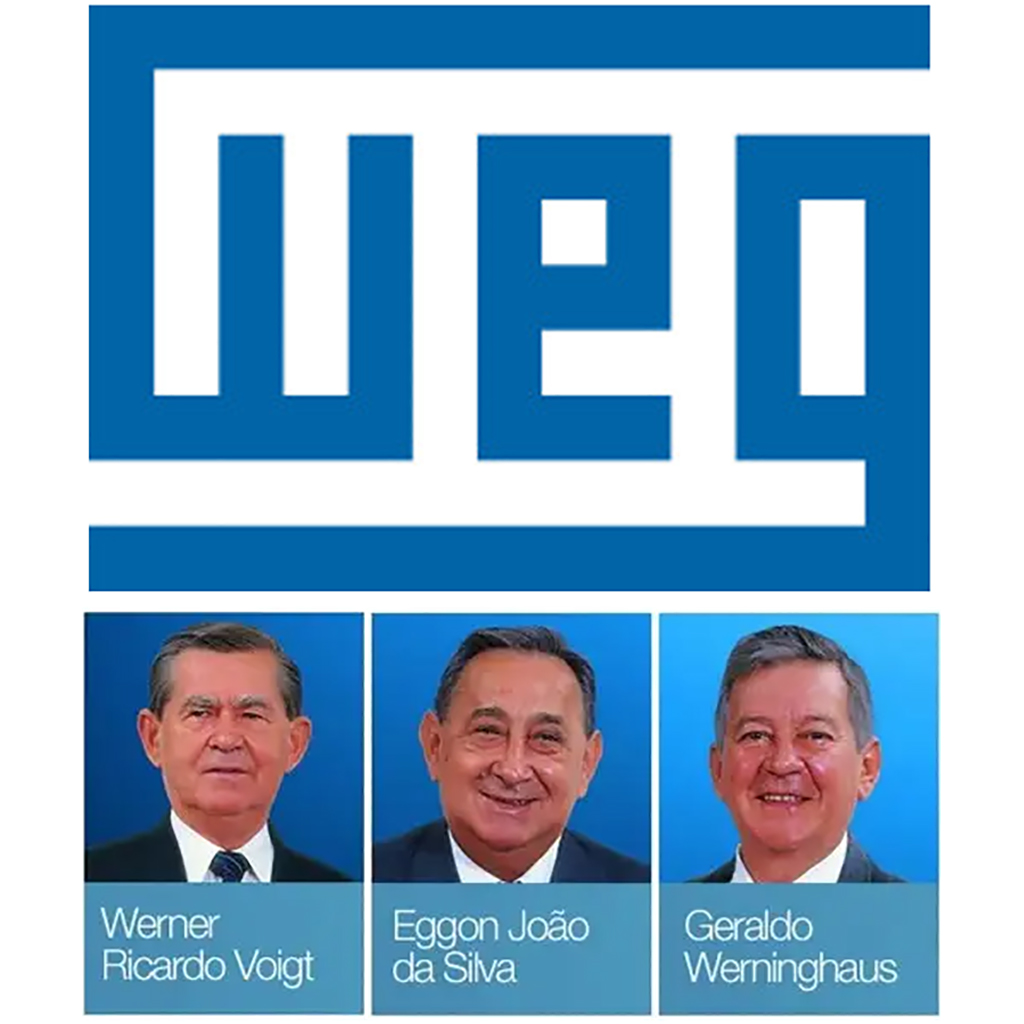
\includegraphics{images/02-2025-08-12_13/02-Weg.jpg} & 
\includegraphics{images/02-2025-08-12_13/022-Tramontina.jpg} \\
\end{longtable}

\begin{center}\rule{0.5\linewidth}{0.5pt}\end{center}

\section{O principal fator é o número efetivo ou potencial de sócios}\label{o-principal-fator-uxe9-o-nuxfamero-efetivo-ou-potencial-de-suxf3cios}

\begin{itemize}
\tightlist
\item
  \textbf{Efetivo:} NÚMERO DE SÓCIOS
\end{itemize}

\begin{longtable}[]{@{}c@{}}
\toprule\noalign{}
\endhead
\bottomrule\noalign{}
\endlastfoot
\textbf{PETROBRÁS} \\
MUITOS, MUITOS SÓCIOS - CAPITAL ABERTO \\
EMPRESA SOCIEDADE ANÔNIMA (S/A) \\
GOVERNO FEDERAL É O MAIOR ACIONISTA ( MAIS DE 50\% DAS AÇÕES) \\
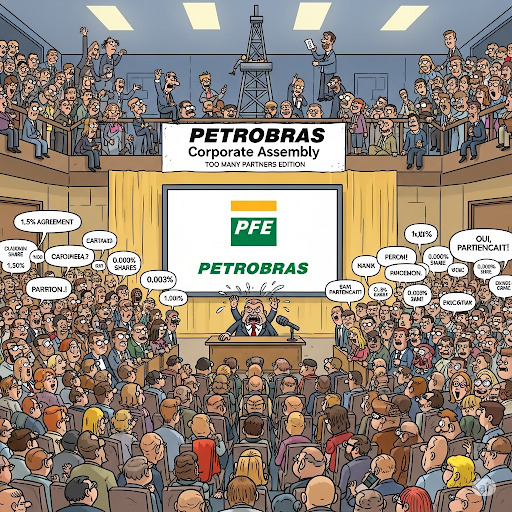
\includegraphics{images/02-2025-08-12_13/00-PetroBras.jpg} \\
\end{longtable}

\begin{center}\rule{0.5\linewidth}{0.5pt}\end{center}

\section{O principal fator é o número efetivo ou potencial de sócios}\label{o-principal-fator-uxe9-o-nuxfamero-efetivo-ou-potencial-de-suxf3cios-1}

\begin{itemize}
\item
  \textbf{Potencial:} futuro número de sócios !

  \begin{longtable}[]{@{}
    >{\centering\arraybackslash}p{(\columnwidth - 2\tabcolsep) * \real{0.3551}}
    >{\centering\arraybackslash}p{(\columnwidth - 2\tabcolsep) * \real{0.6449}}@{}}
  \toprule\noalign{}
  \begin{minipage}[b]{\linewidth}\centering
  POTENCIAL CASO DE AUMENTO DE SÓCIOS
  \end{minipage} & \begin{minipage}[b]{\linewidth}\centering
  \end{minipage} \\
  \midrule\noalign{}
  \endhead
  \bottomrule\noalign{}
  \endlastfoot
  \textbf{FUSÕES} & 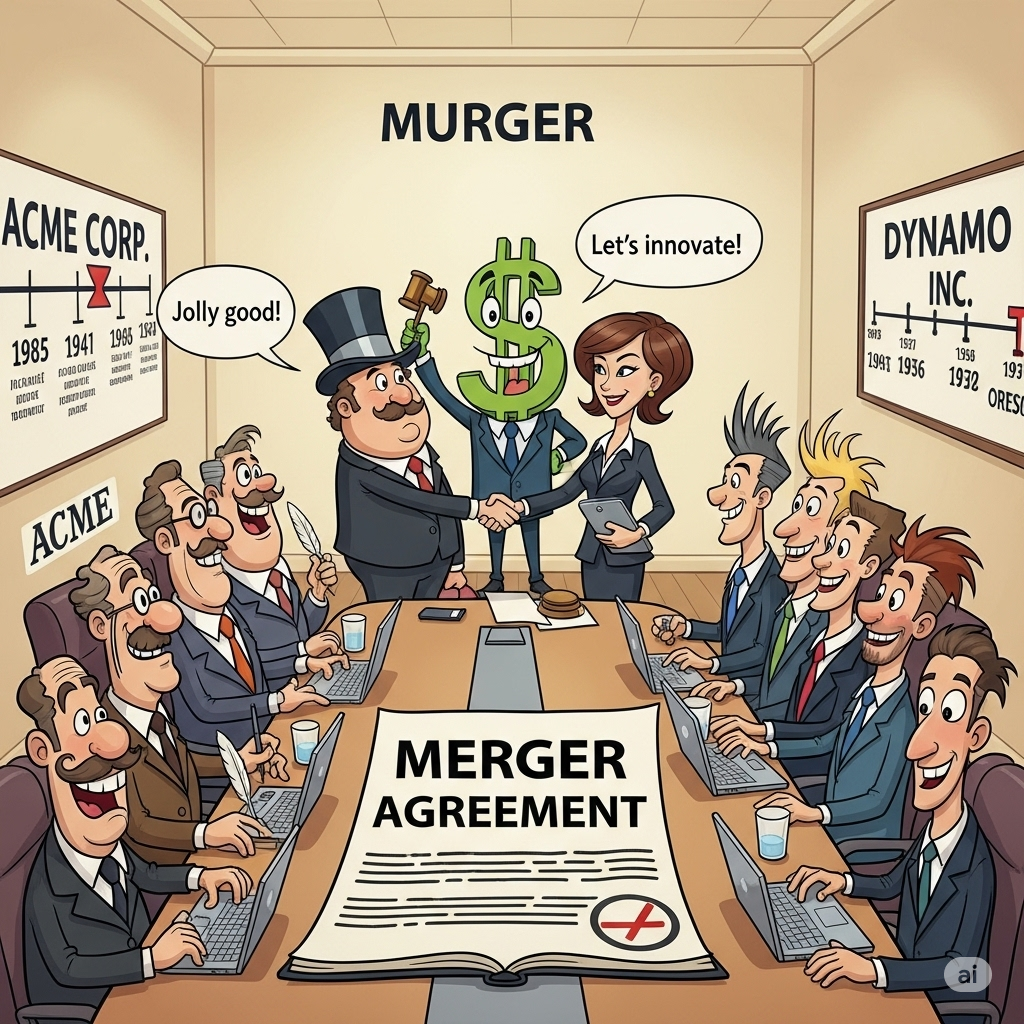
\includegraphics[width=2.46875in,height=\textheight]{images/02-2025-08-12_13/04-Fusao_Corporativa.jpg} \\
  \textbf{AQUISIÇÕES} & \\
  \textbf{INCORPORAÇÕES} & \\
  \textbf{SUCESSÃO FAMILIAR} & \includegraphics[width=1.95833in,height=\textheight]{images/02-2025-08-12_13/03-sucessao_familiar.jpg} \\
  \end{longtable}
\end{itemize}

\begin{center}\rule{0.5\linewidth}{0.5pt}\end{center}

\section{Casos que normalmente demandam arquitetura de governança corporativa}\label{casos-que-normalmente-demandam-arquitetura-de-governanuxe7a-corporativa}

\begin{itemize}
\item
  Sucessão familiar que amplie significativamente o número de sócios\\
  \emph{(filhos -- 1ª geração --, netos -- 2ª geração -- etc.)}

  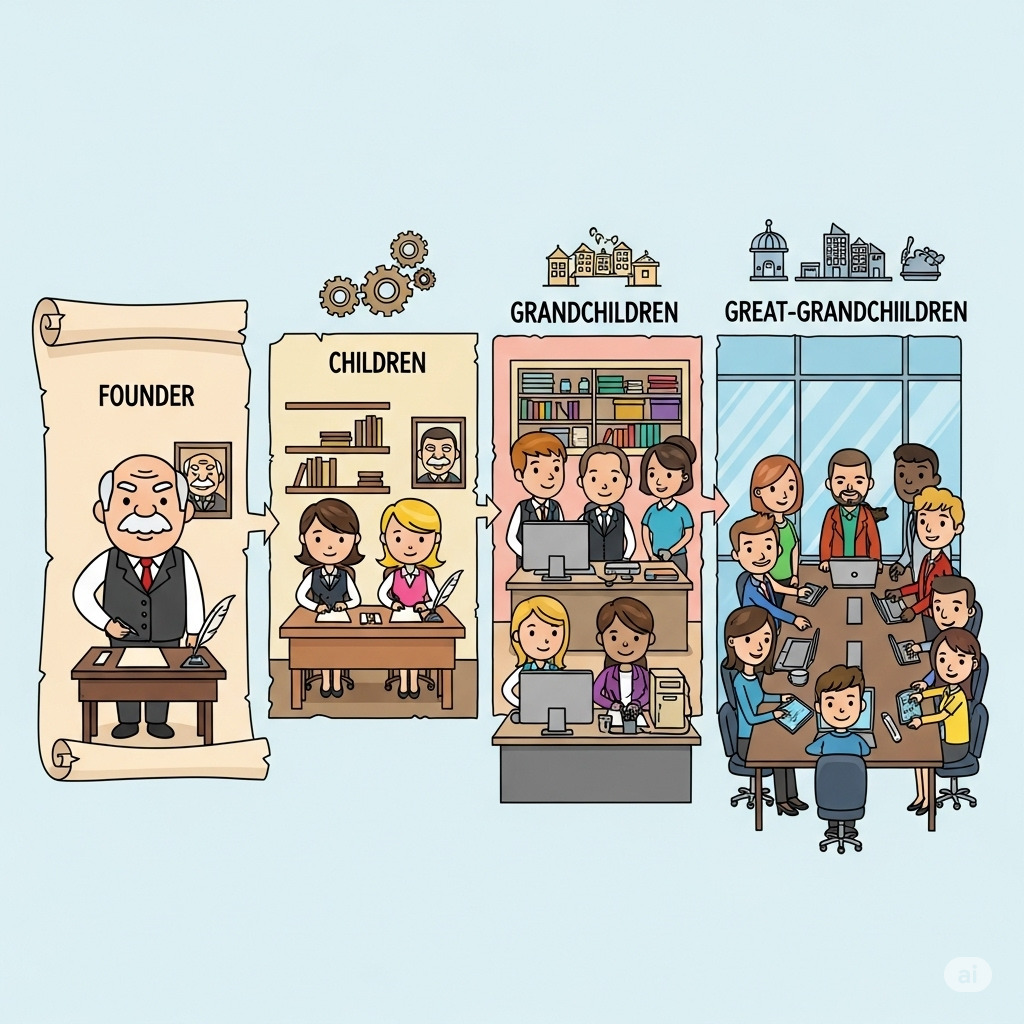
\includegraphics[width=5.69792in,height=\textheight]{images/02-2025-08-12_13/05-linha_sucessoria.jpg}
\item
  Fusão ou incorporação que amplie o número de acionistas ou cotistas
\item
  Sociedade que já nasça com grande número de acionistas ou cotistas
\end{itemize}

\begin{center}\rule{0.5\linewidth}{0.5pt}\end{center}

\section{Arquitetura de Governança}\label{arquitetura-de-governanuxe7a}

\begin{itemize}
\item
  Topo - Assembléia de Acionistas/Cotistas
\item
  2o Degrau - Conselhos (Administrativo, Fiscal e Consultivo)
\item
  3o Degrau - CEO
\item
  4o Degrau - Diretorias
\end{itemize}

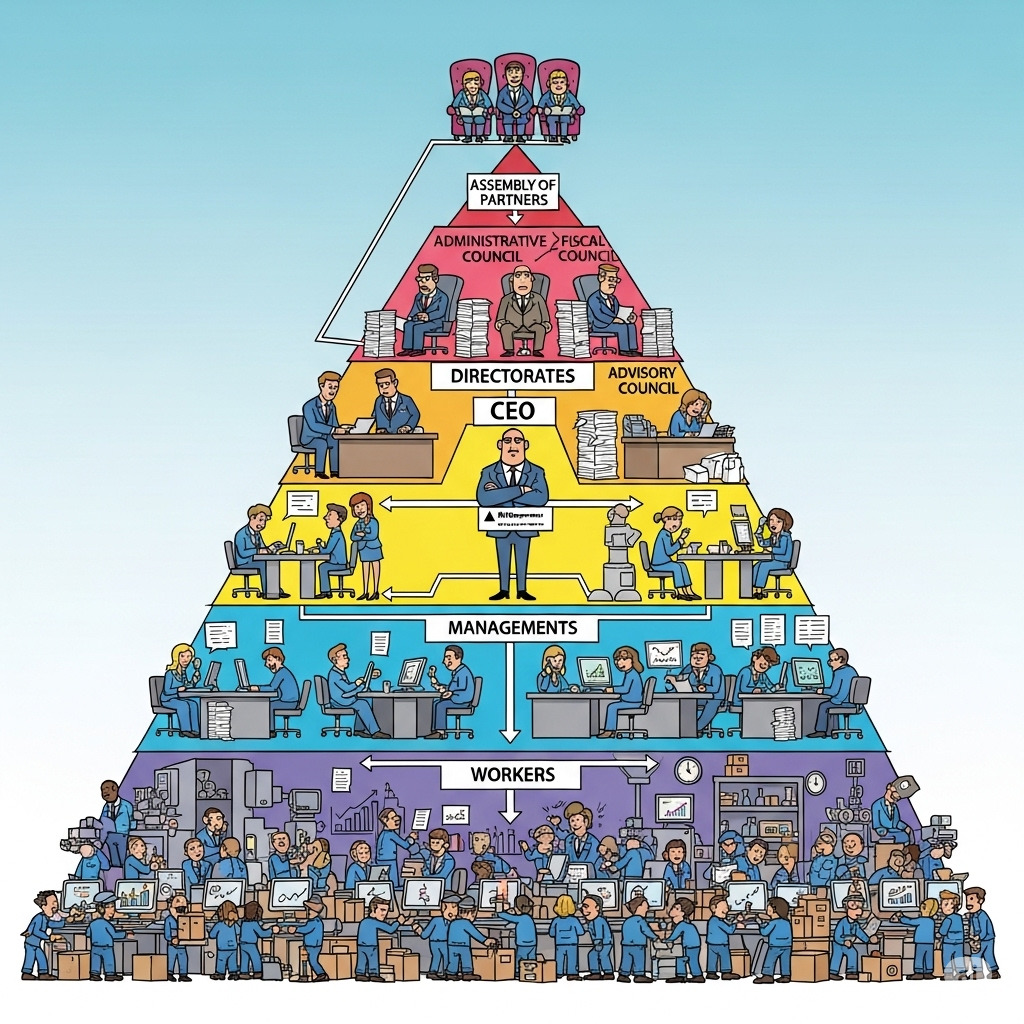
\includegraphics{images/02-2025-08-12_13/00-topo_piramide.jpg}

\begin{center}\rule{0.5\linewidth}{0.5pt}\end{center}

\section{ARQUÉTIPOS DA GOVERNANÇA CORPORATIVA}\label{arquuxe9tipos-da-governanuxe7a-corporativa}

\begin{itemize}
\item
  \textbf{SEPARAÇÃO DE PROPRIEDADE E GESTÃO}
\item
  Anglo-Saxão
\item
  Alemão
\item
  Francês
\item
  Japonês
\item
  Latino-Americano
\end{itemize}

\begin{center}\rule{0.5\linewidth}{0.5pt}\end{center}

\subsubsection{Modelo Anglo-Saxão de Governança Corporativa}\label{modelo-anglo-saxuxe3o-de-governanuxe7a-corporativa}


\includegraphics[width=1.48958in,height=\textheight]{images/02-2025-08-12_13/06-modelo_anglo-saxao.jpg}

\subsection{Características definidoras}\label{caracteruxedsticas-definidoras}

\textbf{Financiamento predominante} - Fonte principal: mercado de capitais - Ações (equity) como base da capitalização - Fundos de pensão com grande parte do patrimônio em ações - Orientação para o mercado

\textbf{Propriedade e controle acionário} - Estrutura patrimonial pulverizada - Raros acionistas com mais de 10\% do capital nas maiores empresas

\textbf{Propriedade e gestão} - Dissociação entre propriedade e gestão

\textbf{Conflitos de agência} - Principal conflito: acionistas x gestores - Altos custos de agência

\textbf{Proteção legal a minoritários} - Forte, por leis e regulação do mercado

\begin{center}\rule{0.5\linewidth}{0.5pt}\end{center}

\subsubsection{Modelo Alemão de Governança Corporativa}\label{modelo-alemuxe3o-de-governanuxe7a-corporativa}


\includegraphics[width=2.34375in,height=\textheight]{images/02-2025-08-12_13/07-modelo_alemao.jpg}

\subsection{Características definidoras}\label{caracteruxedsticas-definidoras-1}

\textbf{Financiamento predominante} - Crédito bancário de longo prazo como principal fonte - Relação duradoura com bancos, reduzindo assimetria de informação

\textbf{Propriedade e controle acionário} - Estrutura patrimonial concentrada - Bancos e grandes acionistas controlam boa parte do capital

\textbf{Propriedade e gestão} - Bancos com grande poder, monitorando interesses dos credores

\textbf{Conflitos de agência} - Principal risco: expropriação de minoritários - Conflitos caros são raros

\textbf{Proteção legal a minoritários} - Não é prioridade; tendência de fortalecer o mercado de ações

\begin{center}\rule{0.5\linewidth}{0.5pt}\end{center}

\subsubsection{Modelo Japonês de Governança Corporativa}\label{modelo-japonuxeas-de-governanuxe7a-corporativa}


\includegraphics[width=2.13542in,height=\textheight]{images/02-2025-08-12_13/09-modelo_japones.jpg}

\subsection{Características definidoras}\label{caracteruxedsticas-definidoras-2}

\textbf{Financiamento predominante} - Bancos financiam via dívida de longo prazo - Relação duradoura entre bancos e empresas

\textbf{Propriedade e controle acionário} - Concentração peculiar: keiretsu com posse cruzada de ações

\textbf{Propriedade e gestão} - Sobreposição; predominância do consenso

\textbf{Conflitos de agência} - Custos e conflitos insignificantes

\textbf{Proteção legal a minoritários} - Sustentação de relações de longo prazo - Gestão voltada a múltiplos interesses

\begin{center}\rule{0.5\linewidth}{0.5pt}\end{center}

\subsubsection{Modelo Francês de Governança Corporativa}\label{modelo-francuxeas-de-governanuxe7a-corporativa}


\includegraphics[width=2.0625in,height=\textheight]{images/02-2025-08-12_13/08-modelo_frances.jpg}

\subsection{Características definidoras}\label{caracteruxedsticas-definidoras-3}

\textbf{Financiamento predominante} - Indefinido, mas alavancagem relevante - Forte presença de empresas familiares fechadas

\textbf{Propriedade e controle acionário} - Controle concentrado

\textbf{Propriedade e gestão} - Sobreposição; gestão fechada - Conselhos com função mais consultiva

\textbf{Conflitos de agência} - Baixos conflitos devido à concentração - Risco de expropriação de minoritários

\textbf{Proteção legal a minoritários} - Fraca, com baixo enforcement - Mercados de capitais pouco desenvolvidos

\begin{center}\rule{0.5\linewidth}{0.5pt}\end{center}

\subsubsection{Modelo Latino-Americano de Governança Corporativa}\label{modelo-latino-americano-de-governanuxe7a-corporativa}


\includegraphics[width=3.1875in,height=\textheight]{images/02-2025-08-12_13/10-modelo_latino_americano.jpg}

\subsection{Características definidoras}\label{caracteruxedsticas-definidoras-4}

\textbf{Financiamento predominante} - Predomínio da dívida - Mercados de capitais pouco expressivos

\textbf{Propriedade e controle acionário} - Propriedade concentrada - Maior participação estrangeira nos últimos anos

\textbf{Propriedade e gestão} - Exercida pelos majoritários

\textbf{Conflitos de agência} - Entre acionistas majoritários e minoritários

\textbf{Proteção legal a minoritários} - Predominantemente fraca - Alta proporção de ações sem voto

\section{Exercícios}\label{exercuxedcios}

\subsection{Testes sobre Modelos de Governança Corporativa}\label{testes-sobre-modelos-de-governanuxe7a-corporativa}

\begin{center}\rule{0.5\linewidth}{0.5pt}\end{center}

Livro \href{https://pdfcoffee.com/governana-corporativa-no-brasil-e-no-mundo-pdf-free.html}{Governança Corporativa no Brasil e no Mundo: Teoria e Prática - Alexandre Di Miceli da SILVEIRA}

Exercícios referentes ao capítulo 1 - Introdução à Governança Corporativa - pág 3 a 6 - Exercícios referentes ao capítulo 2 - Capítulo 2 -- Estrutura de Governança Corporativa - pág 37 a 40 -

\begin{longtable}[]{@{}
  >{\raggedright\arraybackslash}p{(\columnwidth - 0\tabcolsep) * \real{1.0060}}@{}}
\toprule\noalign{}
\begin{minipage}[b]{\linewidth}\raggedright
Questão 1:
\end{minipage} \\
\midrule\noalign{}
\endhead
\bottomrule\noalign{}
\endlastfoot
\textbf{Qual dos seguintes modelos de governança corporativa tem como principal fonte de financiamento o mercado de capitais, com as ações sendo a base da capitalização?} \\
\begin{minipage}[t]{\linewidth}\raggedright
\begin{enumerate}
\def\labelenumi{\alph{enumi})}
\tightlist
\item
  Reduzir custos operacionais internos.
\end{enumerate}
\end{minipage} \\
\begin{minipage}[t]{\linewidth}\raggedright
\begin{enumerate}
\def\labelenumi{\alph{enumi})}
\setcounter{enumi}{1}
\tightlist
\item
  Aumentar o valor da sociedade, facilitar acesso ao capital e garantir perenidade. \textbar{}
\end{enumerate}
\end{minipage} \\
\begin{minipage}[t]{\linewidth}\raggedright
\begin{enumerate}
\def\labelenumi{\alph{enumi})}
\setcounter{enumi}{2}
\tightlist
\item
  Eliminar a necessidade de auditoria independente.
\end{enumerate}
\end{minipage} \\
\begin{minipage}[t]{\linewidth}\raggedright
\begin{enumerate}
\def\labelenumi{\alph{enumi})}
\setcounter{enumi}{3}
\tightlist
\item
  Diminuir a participação dos acionistas minoritários.
\end{enumerate}
\end{minipage} \\
\begin{minipage}[t]{\linewidth}\raggedright
\begin{enumerate}
\def\labelenumi{\alph{enumi})}
\setcounter{enumi}{4}
\tightlist
\item
  Facilitar apenas a sucessão familiar.
\end{enumerate}
\end{minipage} \\
\end{longtable}

\begin{center}\rule{0.5\linewidth}{0.5pt}\end{center}

\begin{longtable}[]{@{}l@{}}
\toprule\noalign{}
\textbf{Questão 2} \\
\midrule\noalign{}
\endhead
\bottomrule\noalign{}
\endlastfoot
\textbf{A implantação de governança corporativa não depende de:} \\
a) Tamanho da empresa. \\
b) Número efetivo ou potencial de sócios. \\
c) Fusões ou incorporações. \\
d) Sucessão familiar. \\
e) Aumento de acionistas minoritários. \\
\end{longtable}

\begin{center}\rule{0.5\linewidth}{0.5pt}\end{center}

\begin{longtable}[]{@{}
  >{\raggedright\arraybackslash}p{(\columnwidth - 0\tabcolsep) * \real{1.0097}}@{}}
\toprule\noalign{}
\begin{minipage}[b]{\linewidth}\raggedright
\textbf{Questão 3}
\end{minipage} \\
\midrule\noalign{}
\endhead
\bottomrule\noalign{}
\endlastfoot
\textbf{Qual é o principal fator para decidir quando implantar uma arquitetura de governança corporativa?} \\
\begin{minipage}[t]{\linewidth}\raggedright
\begin{enumerate}
\def\labelenumi{\alph{enumi})}
\tightlist
\item
  Lucro líquido.
\end{enumerate}
\end{minipage} \\
\begin{minipage}[t]{\linewidth}\raggedright
\begin{enumerate}
\def\labelenumi{\alph{enumi})}
\setcounter{enumi}{1}
\tightlist
\item
  Valor de mercado da empresa.
\end{enumerate}
\end{minipage} \\
\begin{minipage}[t]{\linewidth}\raggedright
\begin{enumerate}
\def\labelenumi{\alph{enumi})}
\setcounter{enumi}{2}
\tightlist
\item
  Número efetivo ou potencial de sócios.
\end{enumerate}
\end{minipage} \\
\begin{minipage}[t]{\linewidth}\raggedright
\begin{enumerate}
\def\labelenumi{\alph{enumi})}
\setcounter{enumi}{3}
\tightlist
\item
  Estrutura de capital de giro.
\end{enumerate}
\end{minipage} \\
\begin{minipage}[t]{\linewidth}\raggedright
\begin{enumerate}
\def\labelenumi{\alph{enumi})}
\setcounter{enumi}{4}
\tightlist
\item
  Taxa de juros do mercado.
\end{enumerate}
\end{minipage} \\
\end{longtable}

\begin{center}\rule{0.5\linewidth}{0.5pt}\end{center}

\begin{longtable}[]{@{}
  >{\raggedright\arraybackslash}p{(\columnwidth - 0\tabcolsep) * \real{1.0118}}@{}}
\toprule\noalign{}
\begin{minipage}[b]{\linewidth}\raggedright
\textbf{Questão 4}
\end{minipage} \\
\midrule\noalign{}
\endhead
\bottomrule\noalign{}
\endlastfoot
\textbf{A sucessão familiar que amplia o número de sócios é um caso típico que demanda:} \\
\begin{minipage}[t]{\linewidth}\raggedright
\begin{enumerate}
\def\labelenumi{\alph{enumi})}
\tightlist
\item
  Expansão internacional.
\end{enumerate}
\end{minipage} \\
\begin{minipage}[t]{\linewidth}\raggedright
\begin{enumerate}
\def\labelenumi{\alph{enumi})}
\setcounter{enumi}{1}
\tightlist
\item
  Arquitetura de governança corporativa.
\end{enumerate}
\end{minipage} \\
\begin{minipage}[t]{\linewidth}\raggedright
\begin{enumerate}
\def\labelenumi{\alph{enumi})}
\setcounter{enumi}{2}
\tightlist
\item
  Troca de CEO.
\end{enumerate}
\end{minipage} \\
\begin{minipage}[t]{\linewidth}\raggedright
\begin{enumerate}
\def\labelenumi{\alph{enumi})}
\setcounter{enumi}{3}
\tightlist
\item
  Criação de novas subsidiárias.
\end{enumerate}
\end{minipage} \\
\begin{minipage}[t]{\linewidth}\raggedright
\begin{enumerate}
\def\labelenumi{\alph{enumi})}
\setcounter{enumi}{4}
\tightlist
\item
  Aumento do capital social.
\end{enumerate}
\end{minipage} \\
\end{longtable}

\begin{center}\rule{0.5\linewidth}{0.5pt}\end{center}

Livro \href{https://pdfcoffee.com/governana-corporativa-no-brasil-e-no-mundo-pdf-free.html}{Governança Corporativa no Brasil e no Mundo: Teoria e Prática - Alexandre Di Miceli da SILVEIRA}

Exercícios referentes ao Capítulo 3 -- Modelos de Governança Corporativa no Mundo - pág 71 a 85 - - Modelo Anglo-Saxão - pág 71 - 74 - Modelo Alemão - pág 74 - 77 - Modelo Japonês - pág 77 - 80 - Modelo Francês - pág 80 - 82 - Modelo Latino-Americano - pág 82 - 85

\begin{center}\rule{0.5\linewidth}{0.5pt}\end{center}

\begin{longtable}[]{@{}
  >{\raggedright\arraybackslash}p{(\columnwidth - 0\tabcolsep) * \real{1.0122}}@{}}
\toprule\noalign{}
\begin{minipage}[b]{\linewidth}\raggedright
\textbf{Questão 5}
\end{minipage} \\
\midrule\noalign{}
\endhead
\bottomrule\noalign{}
\endlastfoot
\textbf{No modelo anglo-saxão, a principal fonte de financiamento das corporações é:} \\
\begin{minipage}[t]{\linewidth}\raggedright
\begin{enumerate}
\def\labelenumi{\alph{enumi})}
\tightlist
\item
  Crédito bancário de longo prazo.
\end{enumerate}
\end{minipage} \\
\begin{minipage}[t]{\linewidth}\raggedright
\begin{enumerate}
\def\labelenumi{\alph{enumi})}
\setcounter{enumi}{1}
\tightlist
\item
  Mercado de capitais.
\end{enumerate}
\end{minipage} \\
\begin{minipage}[t]{\linewidth}\raggedright
\begin{enumerate}
\def\labelenumi{\alph{enumi})}
\setcounter{enumi}{2}
\tightlist
\item
  Recursos familiares.
\end{enumerate}
\end{minipage} \\
\begin{minipage}[t]{\linewidth}\raggedright
\begin{enumerate}
\def\labelenumi{\alph{enumi})}
\setcounter{enumi}{3}
\tightlist
\item
  Capital estatal.
\end{enumerate}
\end{minipage} \\
\begin{minipage}[t]{\linewidth}\raggedright
\begin{enumerate}
\def\labelenumi{\alph{enumi})}
\setcounter{enumi}{4}
\tightlist
\item
  Dívida de fornecedores.
\end{enumerate}
\end{minipage} \\
\begin{minipage}[t]{\linewidth}\raggedright
\begin{enumerate}
\def\labelenumi{\alph{enumi})}
\setcounter{enumi}{4}
\tightlist
\item
  Aumento do capital social.
\end{enumerate}
\end{minipage} \\
\end{longtable}

\begin{center}\rule{0.5\linewidth}{0.5pt}\end{center}

\begin{longtable}[]{@{}
  >{\raggedright\arraybackslash}p{(\columnwidth - 0\tabcolsep) * \real{0.9861}}@{}}
\toprule\noalign{}
\begin{minipage}[b]{\linewidth}\raggedright
\textbf{Questão 6}
\end{minipage} \\
\midrule\noalign{}
\endhead
\bottomrule\noalign{}
\endlastfoot
\textbf{No modelo alemão, o papel dos bancos é:} \\
\begin{minipage}[t]{\linewidth}\raggedright
\begin{enumerate}
\def\labelenumi{\alph{enumi})}
\tightlist
\item
  Inexistente, pois prevalece a pulverização acionária.
\end{enumerate}
\end{minipage} \\
\begin{minipage}[t]{\linewidth}\raggedright
\begin{enumerate}
\def\labelenumi{\alph{enumi})}
\setcounter{enumi}{1}
\tightlist
\item
  Secundário em relação aos fundos de pensão.
\end{enumerate}
\end{minipage} \\
\begin{minipage}[t]{\linewidth}\raggedright
\begin{enumerate}
\def\labelenumi{\alph{enumi})}
\setcounter{enumi}{2}
\tightlist
\item
  Central, como principais financiadores e monitores das empresas.
\end{enumerate}
\end{minipage} \\
\begin{minipage}[t]{\linewidth}\raggedright
\begin{enumerate}
\def\labelenumi{\alph{enumi})}
\setcounter{enumi}{3}
\tightlist
\item
  Consultivo, apenas assessorando conselhos.
\end{enumerate}
\end{minipage} \\
\begin{minipage}[t]{\linewidth}\raggedright
\begin{enumerate}
\def\labelenumi{\alph{enumi})}
\setcounter{enumi}{4}
\tightlist
\item
  Exclusivamente regulatório.
\end{enumerate}
\end{minipage} \\
 \\
\end{longtable}

\begin{center}\rule{0.5\linewidth}{0.5pt}\end{center}

\begin{longtable}[]{@{}
  >{\raggedright\arraybackslash}p{(\columnwidth - 0\tabcolsep) * \real{1.0139}}@{}}
\toprule\noalign{}
\begin{minipage}[b]{\linewidth}\raggedright
\textbf{Questão 7}
\end{minipage} \\
\midrule\noalign{}
\endhead
\bottomrule\noalign{}
\endlastfoot
\textbf{No modelo japonês, a estrutura de propriedade é caracterizada por:} \\
\begin{minipage}[t]{\linewidth}\raggedright
\begin{enumerate}
\def\labelenumi{\alph{enumi})}
\tightlist
\item
  Total pulverização acionária.
\end{enumerate}
\end{minipage} \\
\begin{minipage}[t]{\linewidth}\raggedright
\begin{enumerate}
\def\labelenumi{\alph{enumi})}
\setcounter{enumi}{1}
\tightlist
\item
  Forte controle estatal.
\end{enumerate}
\end{minipage} \\
\begin{minipage}[t]{\linewidth}\raggedright
\begin{enumerate}
\def\labelenumi{\alph{enumi})}
\setcounter{enumi}{2}
\tightlist
\item
  Grupos keiretsu com posse cruzada de ações.
\end{enumerate}
\end{minipage} \\
\begin{minipage}[t]{\linewidth}\raggedright
\begin{enumerate}
\def\labelenumi{\alph{enumi})}
\setcounter{enumi}{3}
\tightlist
\item
  Predomínio de fundos de pensão.
\end{enumerate}
\end{minipage} \\
\begin{minipage}[t]{\linewidth}\raggedright
\begin{enumerate}
\def\labelenumi{\alph{enumi})}
\setcounter{enumi}{4}
\tightlist
\item
  Participação estrangeira majoritária.
\end{enumerate}
\end{minipage} \\
 \\
\end{longtable}

\begin{center}\rule{0.5\linewidth}{0.5pt}\end{center}

\begin{longtable}[]{@{}
  >{\raggedright\arraybackslash}p{(\columnwidth - 0\tabcolsep) * \real{1.0133}}@{}}
\toprule\noalign{}
\begin{minipage}[b]{\linewidth}\raggedright
\textbf{QUESTÃO 8}
\end{minipage} \\
\midrule\noalign{}
\endhead
\bottomrule\noalign{}
\endlastfoot
\textbf{No modelo francês, o conflito de agência é reduzido porque:} \\
\begin{minipage}[t]{\linewidth}\raggedright
\begin{enumerate}
\def\labelenumi{\alph{enumi})}
\tightlist
\item
  A gestão é totalmente terceirizada.
\end{enumerate}
\end{minipage} \\
\begin{minipage}[t]{\linewidth}\raggedright
\begin{enumerate}
\def\labelenumi{\alph{enumi})}
\setcounter{enumi}{1}
\tightlist
\item
  Há forte proteção aos minoritários.
\end{enumerate}
\end{minipage} \\
\begin{minipage}[t]{\linewidth}\raggedright
\begin{enumerate}
\def\labelenumi{\alph{enumi})}
\setcounter{enumi}{2}
\tightlist
\item
  A concentração patrimonial gera sobreposição de propriedade e gestão.
\end{enumerate}
\end{minipage} \\
\begin{minipage}[t]{\linewidth}\raggedright
\begin{enumerate}
\def\labelenumi{\alph{enumi})}
\setcounter{enumi}{3}
\tightlist
\item
  A legislação é baseada no modelo anglo-saxão.
\end{enumerate}
\end{minipage} \\
\begin{minipage}[t]{\linewidth}\raggedright
\begin{enumerate}
\def\labelenumi{\alph{enumi})}
\setcounter{enumi}{4}
\tightlist
\item
  O mercado de capitais é muito desenvolvido.
\end{enumerate}
\end{minipage} \\
 \\
\end{longtable}

\begin{center}\rule{0.5\linewidth}{0.5pt}\end{center}

\begin{longtable}[]{@{}
  >{\raggedright\arraybackslash}p{(\columnwidth - 0\tabcolsep) * \real{1.0116}}@{}}
\toprule\noalign{}
\begin{minipage}[b]{\linewidth}\raggedright
\textbf{Questão 9}
\end{minipage} \\
\midrule\noalign{}
\endhead
\bottomrule\noalign{}
\endlastfoot
\textbf{No modelo latino-americano (brasileiro), qual é o principal conflito de agência?} \\
\begin{minipage}[t]{\linewidth}\raggedright
\begin{enumerate}
\def\labelenumi{\alph{enumi})}
\tightlist
\item
  Entre acionistas e gestores.
\end{enumerate}
\end{minipage} \\
\begin{minipage}[t]{\linewidth}\raggedright
\begin{enumerate}
\def\labelenumi{\alph{enumi})}
\setcounter{enumi}{1}
\tightlist
\item
  Entre bancos e credores.
\end{enumerate}
\end{minipage} \\
\begin{minipage}[t]{\linewidth}\raggedright
\begin{enumerate}
\def\labelenumi{\alph{enumi})}
\setcounter{enumi}{2}
\tightlist
\item
  Entre acionistas majoritários e minoritários.
\end{enumerate}
\end{minipage} \\
\begin{minipage}[t]{\linewidth}\raggedright
\begin{enumerate}
\def\labelenumi{\alph{enumi})}
\setcounter{enumi}{3}
\tightlist
\item
  Entre conselhos e diretoria executiva.
\end{enumerate}
\end{minipage} \\
\begin{minipage}[t]{\linewidth}\raggedright
\begin{enumerate}
\def\labelenumi{\alph{enumi})}
\setcounter{enumi}{4}
\tightlist
\item
  Entre empresas familiares e fundos de pensão.
\end{enumerate}
\end{minipage} \\
\end{longtable}

\begin{center}\rule{0.5\linewidth}{0.5pt}\end{center}

\begin{longtable}[]{@{}l@{}}
\toprule\noalign{}
\textbf{QUESTÃO 10} \\
\midrule\noalign{}
\endhead
\bottomrule\noalign{}
\endlastfoot
\textbf{Em relação à proteção legal dos acionistas minoritários:} \\
a) É forte e predominante no modelo latino-americano. \\
b) É pouco relevante no modelo japonês. \\
c) É expressiva e garantida por regulação no modelo anglo-saxão. \\
d) É garantida pela concentração patrimonial no modelo francês. \\
e) É inexistente no modelo alemão. \\
\end{longtable}

\begin{center}\rule{0.5\linewidth}{0.5pt}\end{center}

\section{Respostas dos exercícios}\label{respostas-dos-exercuxedcios}

\begin{longtable}[]{@{}
  >{\raggedright\arraybackslash}p{(\columnwidth - 2\tabcolsep) * \real{0.1212}}
  >{\raggedright\arraybackslash}p{(\columnwidth - 2\tabcolsep) * \real{0.8788}}@{}}
\toprule\noalign{}
\begin{minipage}[b]{\linewidth}\raggedright
Questão
\end{minipage} & \begin{minipage}[b]{\linewidth}\raggedright
Alternativa Correta
\end{minipage} \\
\midrule\noalign{}
\endhead
\bottomrule\noalign{}
\endlastfoot
\textbf{1} & \begin{minipage}[t]{\linewidth}\raggedright
\begin{enumerate}
\def\labelenumi{\alph{enumi})}
\setcounter{enumi}{1}
\tightlist
\item
  Aumentar o valor da sociedade, facilitar acesso ao capital e garantir perenidade
\end{enumerate}
\end{minipage} \\
\textbf{2} & \begin{minipage}[t]{\linewidth}\raggedright
\begin{enumerate}
\def\labelenumi{\alph{enumi})}
\tightlist
\item
  Tamanho da empresa
\end{enumerate}
\end{minipage} \\
\textbf{3} & \begin{minipage}[t]{\linewidth}\raggedright
\begin{enumerate}
\def\labelenumi{\alph{enumi})}
\setcounter{enumi}{2}
\tightlist
\item
  Número efetivo ou potencial de sócios
\end{enumerate}
\end{minipage} \\
\textbf{4} & \begin{minipage}[t]{\linewidth}\raggedright
\begin{enumerate}
\def\labelenumi{\alph{enumi})}
\setcounter{enumi}{1}
\tightlist
\item
  Arquitetura de governança corporativa
\end{enumerate}
\end{minipage} \\
\textbf{5} & \begin{minipage}[t]{\linewidth}\raggedright
\begin{enumerate}
\def\labelenumi{\alph{enumi})}
\setcounter{enumi}{1}
\tightlist
\item
  Mercado de capitais
\end{enumerate}
\end{minipage} \\
\textbf{6} & \begin{minipage}[t]{\linewidth}\raggedright
\begin{enumerate}
\def\labelenumi{\alph{enumi})}
\setcounter{enumi}{2}
\tightlist
\item
  Central, como principais financiadores e monitores das empresas
\end{enumerate}
\end{minipage} \\
\textbf{7} & \begin{minipage}[t]{\linewidth}\raggedright
\begin{enumerate}
\def\labelenumi{\alph{enumi})}
\setcounter{enumi}{2}
\tightlist
\item
  Grupos keiretsu com posse cruzada de ações
\end{enumerate}
\end{minipage} \\
\textbf{8} & \begin{minipage}[t]{\linewidth}\raggedright
\begin{enumerate}
\def\labelenumi{\alph{enumi})}
\setcounter{enumi}{2}
\tightlist
\item
  A concentração patrimonial gera sobreposição de propriedade e gestão
\end{enumerate}
\end{minipage} \\
\textbf{9} & \begin{minipage}[t]{\linewidth}\raggedright
\begin{enumerate}
\def\labelenumi{\alph{enumi})}
\setcounter{enumi}{2}
\tightlist
\item
  Entre acionistas majoritários e minoritários
\end{enumerate}
\end{minipage} \\
\textbf{10} & \begin{minipage}[t]{\linewidth}\raggedright
\begin{enumerate}
\def\labelenumi{\alph{enumi})}
\setcounter{enumi}{2}
\tightlist
\item
  É expressiva e garantida por regulação no modelo anglo-saxão
\end{enumerate}
\end{minipage} \\
\end{longtable}

\section{Referências}\label{referuxeancias}

ROSSETTI, José Paschoal; ANDRADE, Adriana. \emph{Governança Corporativa: Fundamentos, Desenvolvimento e Tendências}. São Paulo: Atlas, 7. ed., 2014. p.~s.p.

SILVEIRA, Alexandre Di Miceli da. \emph{Governança Corporativa no Brasil e no Mundo: Teoria e Prática}. Rio de Janeiro: Elsevier, 2010.

\chapter{Governança Corporativa - Assembléia dos Proprietários}\label{governanuxe7a-corporativa---assembluxe9ia-dos-proprietuxe1rios}

\subsubsection*{19/08/2025 - Campus Marquês}\label{campus-marquuxeas-2}
\addcontentsline{toc}{subsubsection}{19/08/2025 - Campus Marquês}

\subsubsection*{20/08/2025 - Campus Chácara}\label{campus-chuxe1cara-2}
\addcontentsline{toc}{subsubsection}{20/08/2025 - Campus Chácara}

\subsection{Livro ``Governança Corporativa''}\label{livro-governanuxe7a-corporativa}

\subsubsection{capítulo ``A Assembleia Geral no processo de governança'', pág 267}\label{capuxedtulo-a-assembleia-geral-no-processo-de-governanuxe7a-puxe1g-267}

\section{\texorpdfstring{\textbf{A Assembleia Geral}}{A Assembleia Geral}}\label{a-assembleia-geral}

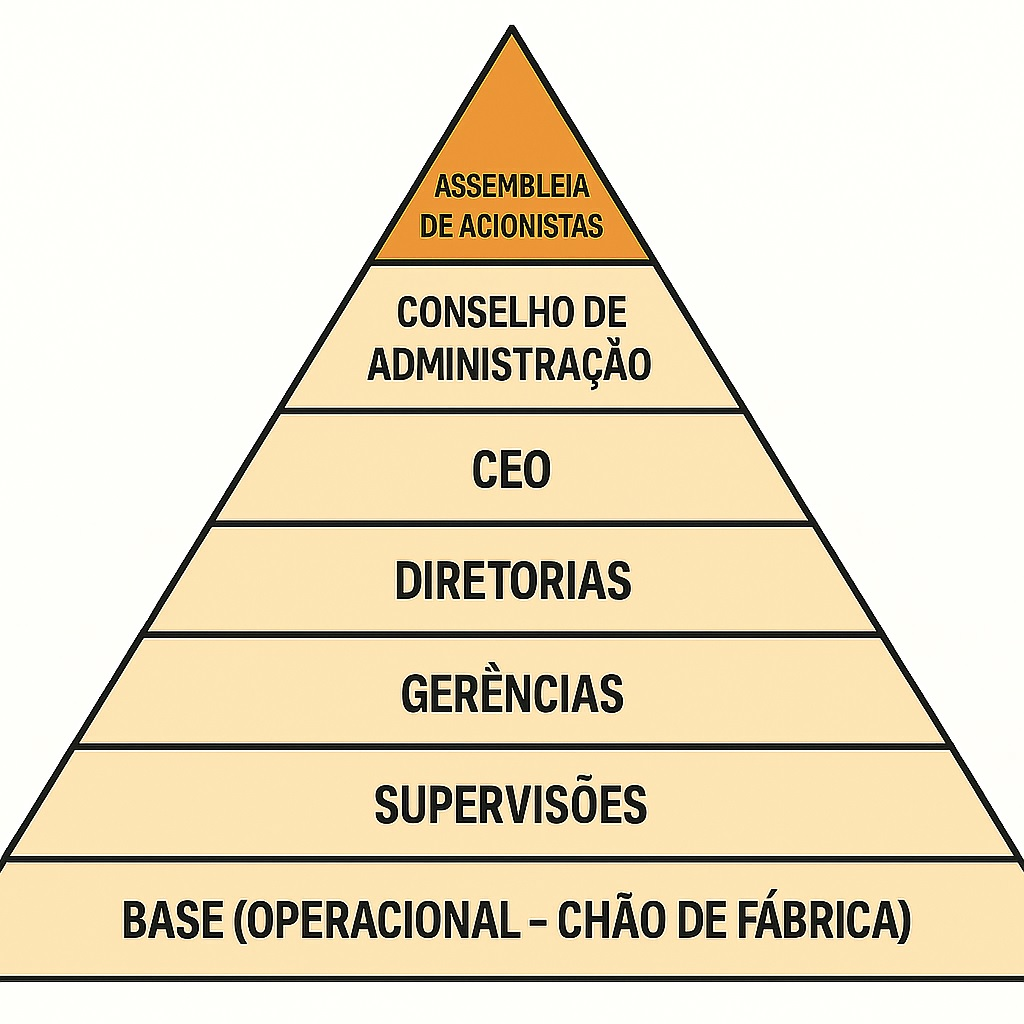
\includegraphics[width=5.34375in,height=\textheight]{images/03-2025-08-19_20/00-assembleia_cotistas.jpg}

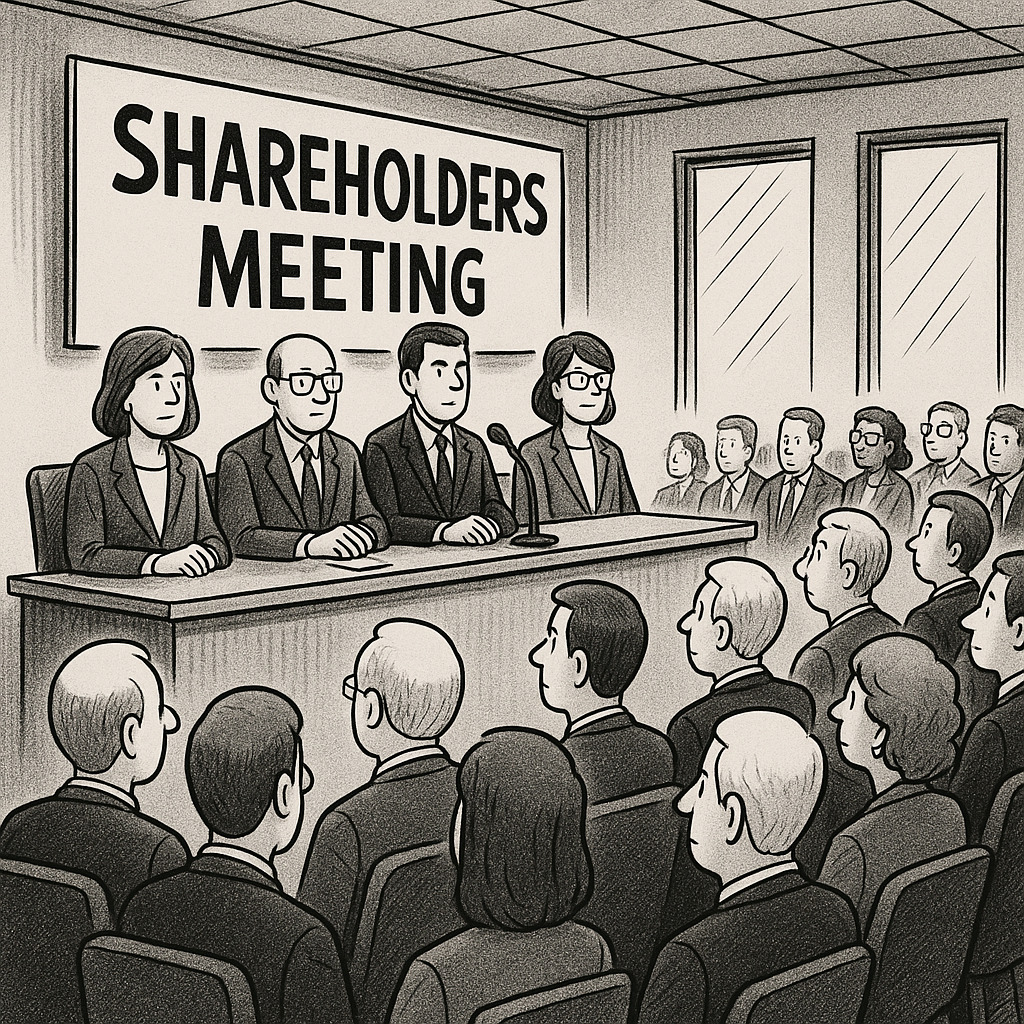
\includegraphics[width=5.36458in,height=\textheight]{images/03-2025-08-19_20/01-assembleia_cotistas.jpg}

É definida como a \textbf{reunião de acionistas ou cotistas}.

É considerada o \textbf{órgão soberano da organização}.

\section{\texorpdfstring{\textbf{Principais Competências da Assembleia Geral}}{Principais Competências da Assembleia Geral}}\label{principais-competuxeancias-da-assembleia-geral}

As competências destacadas da Assembleia Geral incluem:

\begin{itemize}
\item
  \textbf{Aumentar ou reduzir o capital social} e \textbf{reformar o estatuto/contrato social}.
\item
  \textbf{Eleger ou destituir}, a qualquer tempo, \textbf{conselheiros de administração e fiscais}.
\item
  Tomar, anualmente, as \textbf{contas dos administradores} e deliberar sobre as \textbf{demonstrações financeiras}.
\item
  Deliberar sobre \textbf{transformação, fusão, incorporação, cisão, dissolução e liquidação da sociedade}.
\item
  Deliberar sobre a \textbf{avaliação de bens} que venham a integralizar o capital social.
\item
  \textbf{Aprovar a remuneração dos administradores}.
\end{itemize}

\section{\texorpdfstring{\textbf{Frequência e Modalidade das Assembleias}}{Frequência e Modalidade das Assembleias}}\label{frequuxeancia-e-modalidade-das-assembleias}

A Assembleia Geral pode ser de dois tipos, elecandos abaixo:

\subsection{\texorpdfstring{\textbf{Assembleia Geral Ordinária (AGO)}}{Assembleia Geral Ordinária (AGO)}}\label{assembleia-geral-ordinuxe1ria-ago}

Ocorre uma vez por ano com o objetivo de \textbf{aprovar as contas do exercício e o planejamento do ano seguinte}.

\subsection{\texorpdfstring{\textbf{Assembleia Geral Extraordinária (AGE)}}{Assembleia Geral Extraordinária (AGE)}}\label{assembleia-geral-extraordinuxe1ria-age}

Pode ocorrer a qualquer momento, \textbf{sendo convocada por administradores ou acionistas/cotistas}, de acordo com as regras previstas no estatuto social.

\begin{center}\rule{0.5\linewidth}{0.5pt}\end{center}

\section{Participação Patromonial na empresa (Equity)}\label{participauxe7uxe3o-patromonial-na-empresa-equity}

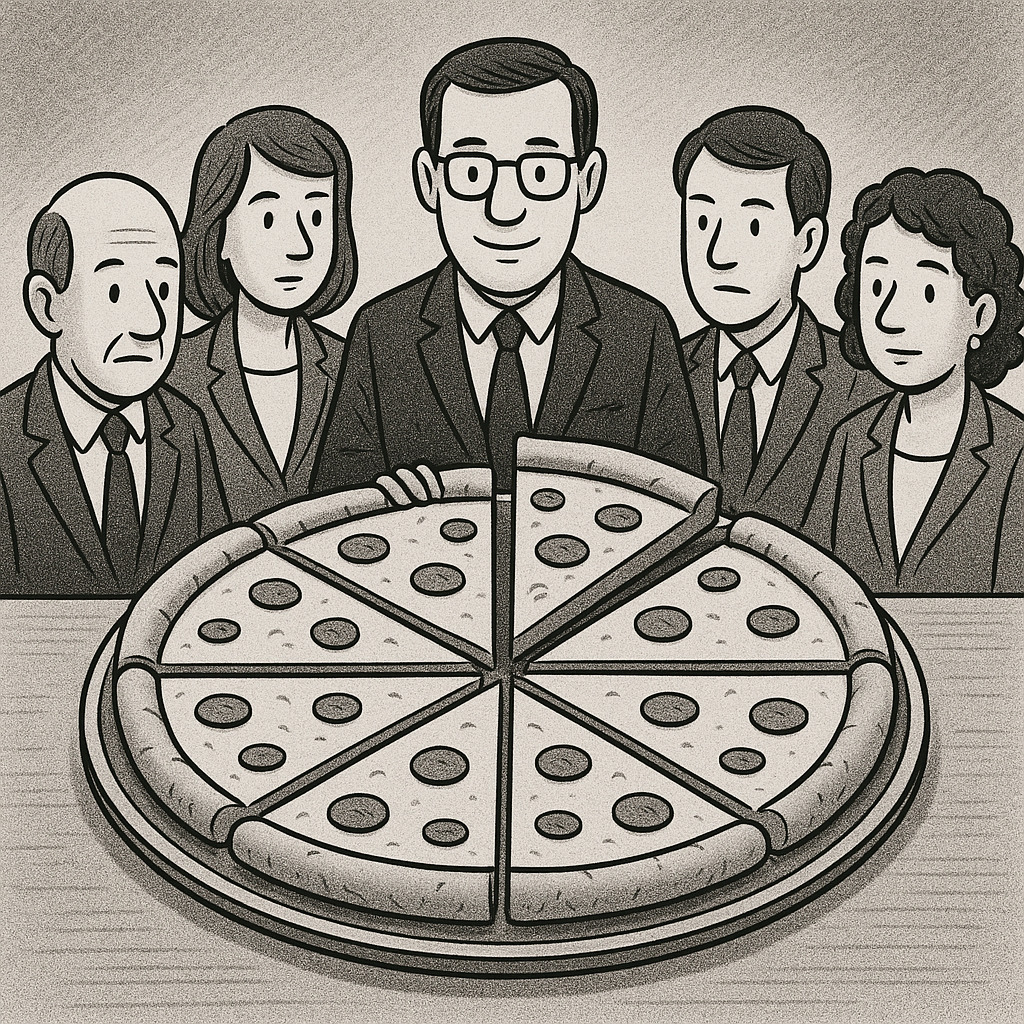
\includegraphics[width=2.3125in,height=\textheight]{images/03-2025-08-19_20/02-assembleia_cotistas-equity.jpg}

\subsubsection{Como calcular EQUITY após uma rodada de investimentos}\label{como-calcular-equity-apuxf3s-uma-rodada-de-investimentos}

Como um acionista pode calcular sua participação na empresa após uma rodada de investimentos ?

Basicamente, podemos fazer-lo aplicado a fórmula:

\subsubsection{Participação percentual do sócio pós-seção de participação ao investidor}\label{participauxe7uxe3o-percentual-do-suxf3cio-puxf3s-seuxe7uxe3o-de-participauxe7uxe3o-ao-investidor}

\[
Porcentagem\_Participacao\_Sócio\_Pós\_Investimento = \frac{Porcentagem\_Participacao\_Pré\_Investimento}{(1 - Participacao\_Percentual\_Investidor)}
\]

\subsubsection{Participação percentual do investidor pós-investimento monetário}\label{participauxe7uxe3o-percentual-do-investidor-puxf3s-investimento-monetuxe1rio}

\[
Participação\_Percentual\_\_Investidor = (\frac{ Dinheiro\_Investido}{ CapitalSocial\_Pós\_Investimento}) * 100%
\]

\section{Equity - caso FACEBOOK}\label{equity---caso-facebook}

\url{https://www.youtube.com/watch?v=YR4eE9TVq44&t=194s}


\includegraphics[width=7.04167in,height=\textheight]{images/03-2025-08-19_20/05-facebook.png}

\begin{longtable}[]{@{}
  >{\raggedright\arraybackslash}p{(\columnwidth - 2\tabcolsep) * \real{0.5442}}
  >{\raggedright\arraybackslash}p{(\columnwidth - 2\tabcolsep) * \real{0.4558}}@{}}
\toprule\noalign{}
\endhead
\bottomrule\noalign{}
\endlastfoot
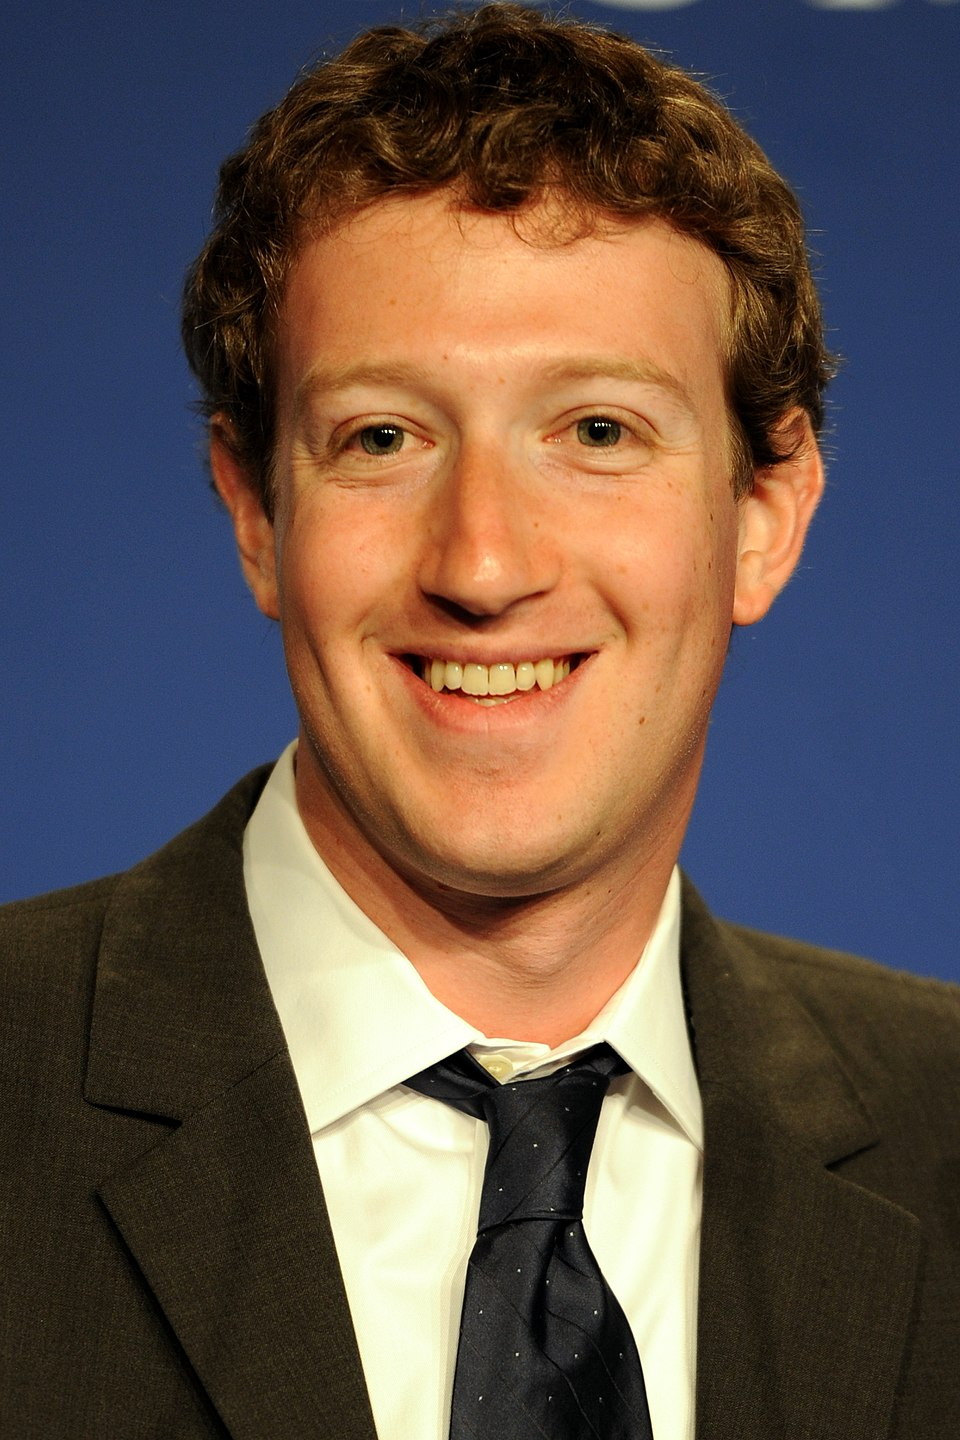
\includegraphics[width=3.4375in,height=4.30208in]{images/03-2025-08-19_20/03-mark_zuckenberg.jpg} & 
\includegraphics[width=3.95833in,height=\textheight]{images/03-2025-08-19_20/04-eduardo_saverin.jpg} \\
\end{longtable}

\begin{longtable}[]{@{}
  >{\raggedright\arraybackslash}p{(\columnwidth - 6\tabcolsep) * \real{0.0680}}
  >{\raggedright\arraybackslash}p{(\columnwidth - 6\tabcolsep) * \real{0.1054}}
  >{\raggedright\arraybackslash}p{(\columnwidth - 6\tabcolsep) * \real{0.0816}}
  >{\raggedright\arraybackslash}p{(\columnwidth - 6\tabcolsep) * \real{0.7381}}@{}}
\toprule\noalign{}
\begin{minipage}[b]{\linewidth}\raggedright
Data (Estim)
\end{minipage} & \begin{minipage}[b]{\linewidth}\raggedright
Evento Chave
\end{minipage} & \begin{minipage}[b]{\linewidth}\raggedright
Equity Saverin(Estim)
\end{minipage} & \begin{minipage}[b]{\linewidth}\raggedright
Contexto e Ação
\end{minipage} \\
\midrule\noalign{}
\endhead
\bottomrule\noalign{}
\endlastfoot
Fevereiro de 2004 & Fundação do Facebook & 30\% a 34\% & \textbf{Eduardo Saverin} investe \textbf{US\$ 15 mil} para ajudar a fundar a empresa. \textbf{Sua participação é a maior entre os sócios}, atrás apenas de \textbf{Mark Zuckerberg}. \\
Metade de 2004 & Mudança para Palo Alto & \textless{} 30\% & Desentendimentos entre Zuckerberg e Saverin. Zuckerberg começa a buscar novos investidores e a estruturar a empresa legalmente para uma nova rodada de investimento. \\
Junho de 2004 & Aporte de Peter Thiel & \textasciitilde20\% a 25\% & \textbf{Peter Thiel} e \textbf{Reid Hoffman} (investidores-anjo) injetam \textbf{US\$ 500 mil} no Facebook. Esta é a primeira rodada de investimento que causa a diluição da participação dos fundadores. \\
Final de 2004 & Reestruturação e Exclusão & \textless{} 10\% & \textbf{Zuckerberg} cria uma \textbf{nova entidade legal} (``Thefacebook, Inc.''), emite novas ações e, de forma controversa, \textbf{dilui a participação de Saverin} a uma porcentagem mínima \textbf{sem seu consentimento}. \\
Maio de 2005 & Rodada de Série A & \textasciitilde10\% & A \textbf{Accel Partners} e o co-fundador da PayPal investem \textbf{US\$ 12,7 milhões} na empresa. \textbf{Ações adicionais são emitidas}, \textbf{diluindo ainda mais todos os fundadores}, incluindo \textbf{Saverin}. \\
Setembro de 2005 & Processo Judicial de Saverin & \textasciitilde10\% & \textbf{Saverin} processa \textbf{Zuckerberg} e o Facebook, alegando que \textbf{foi diluído de forma ilegal} e \textbf{quebra de contrato}. \\
2006 & Rodada de Série B & \textless{} 10\% & \textbf{Accel Partners}, \textbf{Greylock Partners} e outros \textbf{investem US\$ 27,5 milhões}. A diluição continua. \\
2007 & Rodada da Microsoft & \textless{} 5\% & \textbf{A Microsoft investe US\$ 240 milhões}, avaliando o \textbf{Facebook em US\$ 15 bilhões}. A \textbf{emissão de novas ações dilui drasticamente a participação de todos os sócios}. \\
2008 & Acordo com Saverin & \textasciitilde4\% & Saverin e Zuckerberg chegam a um acordo extrajudicial. Os termos exatos não são revelados, mas é noticiado que Saverin recebe uma quantia em dinheiro, suas ações são restauradas, e ele é readmitido como cofundador. \\
Maio de 2012 & IPO do Facebook & \textasciitilde2\% & No momento da \textbf{Oferta Pública Inicial (IPO)}, a participação de Saverin é amplamente divulgada como \textbf{estando em torno de 2\%}. O \textbf{valor de sua fatia é estimado em cerca de US\$ 4 bilhões}. \\
& & & \\
\end{longtable}

\begin{center}\rule{0.5\linewidth}{0.5pt}\end{center}

\section{Exemplo}\label{exemplo}

\begin{center}\rule{0.5\linewidth}{0.5pt}\end{center}

\section{Exercício Resolvido 1}\label{exercuxedcio-resolvido-1}

(Etapa 2 de Investimento: tipo Seed Capital -\textgreater{} Investidor ``Anjo'')

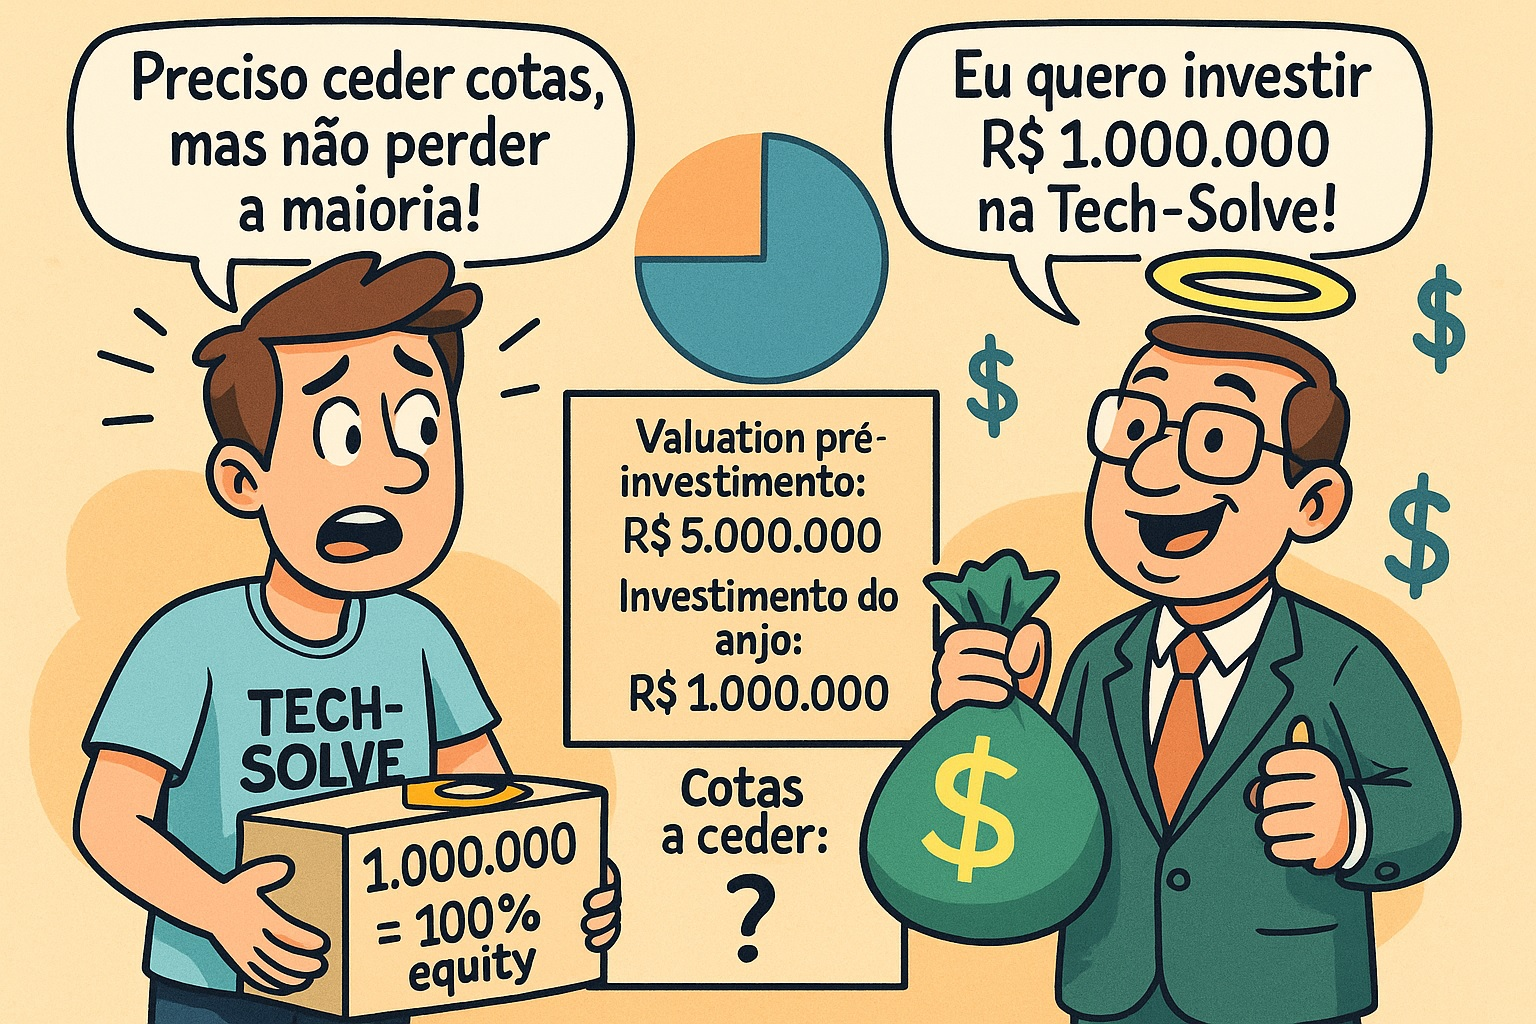
\includegraphics[width=7.125in,height=\textheight]{images/03-2025-08-19_20/exercicio-01.jpg}

\begin{longtable}[]{@{}
  >{\raggedright\arraybackslash}p{(\columnwidth - 0\tabcolsep) * \real{1.0027}}@{}}
\toprule\noalign{}
\endhead
\bottomrule\noalign{}
\endlastfoot
\begin{minipage}[t]{\linewidth}\raggedright
EXEMPLO 1 - Você é o único fundador da startup ``\textbf{Tech-Solve}'' e possui 1.000.000 (um mihão) de cotas da empresa, que representam 100\% do \textbf{EQUITY}. Um investidor anjo (seed capital) se interessa em investir. O valuation (valor da empresa antes do investimento) é de \textbf{R\$ 5.000.000,00} . O investidor quer injetar um capital de \textbf{R\$ 1.000.000} na empresa. Descubra:

\begin{enumerate}
\def\labelenumi{\Roman{enumi})}
\item
  Com quantas cotas o fundador original ficou após o aporte (investimento) de R\$ 1.000.000,00 (um milhão de reiais) ?
\item
  Qual a participação no Capital Social da empresa de cada sócio após o investimento ?
\item
  Quantas cotas receberá o investidor ( então novo sócio da \textbf{Tech-Solve}) após o seu investimento ?
\item
  Qual o valor máximo que um investidor poderia aportar (colocar na empresa), sem que o dono original perca a majoridade ?
\end{enumerate}

Para \textbf{não perder a maioria}, qual o \textbf{número máximo de cotas} você pode ceder a ele, considerando que cada cota tem um valor unitário?
\end{minipage} \\
\end{longtable}

\subsection{Resolução do Exercício I:}\label{resoluuxe7uxe3o-do-exercuxedcio-i}

\subsubsection{Item I - Com quantas cotas o fundador original ficou após o aporte (investimento) de R\$ 1.000.000,00 (um milhão de reiais) ?}\label{item-i---com-quantas-cotas-o-fundador-original-ficou-apuxf3s-o-aporte-investimento-de-r-1.000.00000-um-milhuxe3o-de-reiais}

\begin{longtable}[]{@{}
  >{\raggedright\arraybackslash}p{(\columnwidth - 6\tabcolsep) * \real{0.1905}}
  >{\centering\arraybackslash}p{(\columnwidth - 6\tabcolsep) * \real{0.1714}}
  >{\centering\arraybackslash}p{(\columnwidth - 6\tabcolsep) * \real{0.2381}}
  >{\centering\arraybackslash}p{(\columnwidth - 6\tabcolsep) * \real{0.3810}}@{}}
\toprule\noalign{}
\begin{minipage}[b]{\linewidth}\raggedright
Sócio em Análise
\end{minipage} & \begin{minipage}[b]{\linewidth}\centering
COTAS ANTES
\end{minipage} & \begin{minipage}[b]{\linewidth}\centering
INVESTIMENTO
\end{minipage} & \begin{minipage}[b]{\linewidth}\centering
COTAS DEPOIS
\end{minipage} \\
\midrule\noalign{}
\endhead
\bottomrule\noalign{}
\endlastfoot
Sócio original

(Sócio-Fundador) & \textbf{\emph{1.000.000}} & N/A & \textbf{\emph{1.000.000}} \\
Sócio atual

(Investidor-Anjo) & \textbf{0} & \textbf{\emph{R\$ 1.000.000,00}} & (ainda não sabemos) - calcular depois \\
\end{longtable}

\subsubsection{RESPOSTA ITEM I : ``O antigo dono continuar com 1.000.000 (um milhão) de cotas''.}\label{resposta-item-i-o-antigo-dono-continuar-com-1.000.000-um-milhuxe3o-de-cotas.}

\begin{center}\rule{0.5\linewidth}{0.5pt}\end{center}

\subsubsection{Item II - Qual a participação no Capital Social da empresa de cada sócio após o investimento ?}\label{item-ii---qual-a-participauxe7uxe3o-no-capital-social-da-empresa-de-cada-suxf3cio-apuxf3s-o-investimento}

A participação do investidor é a porcentagem que o valor do aporte representa no valor da empresa após o aporte.

\begin{longtable}[]{@{}
  >{\raggedright\arraybackslash}p{(\columnwidth - 6\tabcolsep) * \real{0.2062}}
  >{\centering\arraybackslash}p{(\columnwidth - 6\tabcolsep) * \real{0.2577}}
  >{\centering\arraybackslash}p{(\columnwidth - 6\tabcolsep) * \real{0.2577}}
  >{\centering\arraybackslash}p{(\columnwidth - 6\tabcolsep) * \real{0.2577}}@{}}
\caption{CAPITAL SOCIAL DA EMPRESA Total após o investimento: \textbf{\emph{R\$ 6.000.000,00.}}}\tabularnewline
\toprule\noalign{}
\begin{minipage}[b]{\linewidth}\raggedright
Sócio em Análise
\end{minipage} & \begin{minipage}[b]{\linewidth}\centering
CAPITAL SOCIAL ANTES
\end{minipage} & \begin{minipage}[b]{\linewidth}\centering
INVESTIMENTO
\end{minipage} & \begin{minipage}[b]{\linewidth}\centering
CAPITAL SOCIAL DEPOIS
\end{minipage} \\
\midrule\noalign{}
\endfirsthead
\toprule\noalign{}
\begin{minipage}[b]{\linewidth}\raggedright
Sócio em Análise
\end{minipage} & \begin{minipage}[b]{\linewidth}\centering
CAPITAL SOCIAL ANTES
\end{minipage} & \begin{minipage}[b]{\linewidth}\centering
INVESTIMENTO
\end{minipage} & \begin{minipage}[b]{\linewidth}\centering
CAPITAL SOCIAL DEPOIS
\end{minipage} \\
\midrule\noalign{}
\endhead
\bottomrule\noalign{}
\endlastfoot
Sócio original

(Sócio-Fundador) & \textbf{\emph{R\$ 5.000.000,00}} & N/A & \textbf{\emph{R\$ 5.000.000,00}} \\
Sócio atual

(Investidor-Anjo) & \textbf{R\$ 0,00} & \textbf{\emph{R\$ 1.000.000,00}} & \textbf{\emph{R\$ 1.000.000,00}} \\
\end{longtable}

\[
\textbf{INICIALMENTE} \\
\text{ } \\
\text{ Capital Social total ORIGINAL (todo patrimônio do único dono original) } \\ 
R\$ 5.000.000,00 \quad \rightarrow  100\%
\text{ } \\
\text{ } \\
\textbf{AGORA - APÓS ENTRADA DO NOVO SÓCIO} \\
\text{ } \\
\text{Capital Social total FINAL (após o investimento de 1 milhão) } \\ 
R\$ 6.000.000,00  \quad \rightarrow  100\%
\]

6 milhões é o dinheiro dos dois sócios somados. Destes R\$ 6 milhões totais, a parte do sócio original continua sendo R\$ 5 milhões.

Assim podemos usar a regra de 3

\[
\frac{R\$ 6.000.000,00}{R\$ 5.000.000,00} = \frac{100\%}{x}
\]

Resolvendo:

\[
\textbf{Calculando a fatia de participação do dono original.} \\
\text{ } \\
x = \frac{(R\$ 5.000.000,00) \times 100}{R\$ 6.000.000,00} \\
x = (\frac{5}{6}) \times 100 \\
x \quad = \quad (0,8333 \times 100) \quad = \quad 83,33\%  \\
\textbf{Portanto, 83,33% é agora participação de capital social restante ao dono original.} \\
\text{ } \\
ParticipaçãoInvestidor = (\frac{ R$ 1.000.000}{ R$ 6.000.000}) * 100% \\
\]

\[
\text{-----------------------------------------} \\
\text{ CAPITAL SOCIAL DA EMPRESA INICIALMENTE  } \\
\text{-----------------------------------------} \\
\text{ } \\
\text{Capital Social total ORIGINAL todo patrimônio do unico dono original } \rightarrow \text{ R \$ 5.000.000,00 } \rightarrow \text{ 100\% } \\
\text{ } \\
\text{-------------------------------------------------------} \\
\text{ CAPITAL SOCIAL DA EMPRESA  APÓS ENTRADA DO NOVO SÓCIO } \\
\text{-------------------------------------------------------} \\
\text{ } \\
\text{Capital Social total FINAL (após o investimento de 1 MILHÃO ) } \rightarrow \text{ R\$ 6.000.000,00} \rightarrow \text{ 100\% } \\
\text{ } \\
\text{6 milhões é o dinheiro dos DOIS SÓCIOS SOMADOS} \\
\text{ } \\
\text{ } \\
\text{----------------------------------------------------------------} \\
\text{ PARTICIPAÇÃO DO ANTIGO SÓCIO NO NOVO CAPITAL SOCIAL DA EMPRESA } \\
\text{----------------------------------------------------------------} \\
\text{ } \\
\text{ aplicamos Regra de 3 } \\
\text{ } \\
\text{----------------} \\
\qquad\frac{ R\$ 6.000.000,00 }{ R\$ 5.000.000,00}= \frac{ 100 \% }{x} \qquad \Rightarrow \qquad
x=\frac{ [ (R\$ 5.000.000,00) * (100) ] }{ R\$ 6.000.000,00 } \\
\text{ } \\
x=\frac{ 5 }{6} * 100 \\
\text{ } \\
x= (0,833333) * 100 \\
\text{ } \\
x= 83,33\% \\
\text{ O antigo dono, agora um sócio-fundador, possui } \quad \textbf{83,33%} \quad \text{de participação na empresa} \\
\text{ } \\
\text{----------------------------------------------------------------------------------------------} \\
\text{ PARTICIPAÇÃO DO NOVO SÓCIO (o que entrou como investidior) NO NOVO CAPITAL SOCIAL DA EMPRESA } \\
\text{----------------------------------------------------------------------------------------------} \\
\text{ } \\
\text{ aplicando novamente Regra de 3 } \\
\text{ } \\
\text{----------------} \\
\qquad\frac{ R\$ 6.000.000,00 }{ R\$ 1.000.000,00}= \frac{ 100 \% }{x} \qquad \Rightarrow \qquad
x=\frac{ [ (R\$ 1.000.000,00) * (100) ] }{ R\$ 6.000.000,00 } \\
\text{ } \\
x=\frac{ 1 }{6} * 100 \\
\text{ } \\
x= (0,16666666666) * 100 \\
\text{ } \\
x= 16,6666\% \\
\text{ O novo sócio, agora um sócio-investidor, possui } \quad \textbf{16,66%} \quad \text{de participação na empresa} \\
\text{ } \\
\]

\begin{longtable}[]{@{}
  >{\raggedright\arraybackslash}p{(\columnwidth - 4\tabcolsep) * \real{0.1368}}
  >{\raggedright\arraybackslash}p{(\columnwidth - 4\tabcolsep) * \real{0.4017}}
  >{\raggedright\arraybackslash}p{(\columnwidth - 4\tabcolsep) * \real{0.4530}}@{}}
\caption{Divisão de Percentual de Capital Social}\tabularnewline
\toprule\noalign{}
\begin{minipage}[b]{\linewidth}\raggedright
Sócios
\end{minipage} & \begin{minipage}[b]{\linewidth}\raggedright
Posse do Capital Social

Antes do Investidor ejetar dinheiro (aporte)
\end{minipage} & \begin{minipage}[b]{\linewidth}\raggedright
Posse do Capital Social

Depois do novo investidor ejetar dinheiro (aporte)
\end{minipage} \\
\midrule\noalign{}
\endfirsthead
\toprule\noalign{}
\begin{minipage}[b]{\linewidth}\raggedright
Sócios
\end{minipage} & \begin{minipage}[b]{\linewidth}\raggedright
Posse do Capital Social

Antes do Investidor ejetar dinheiro (aporte)
\end{minipage} & \begin{minipage}[b]{\linewidth}\raggedright
Posse do Capital Social

Depois do novo investidor ejetar dinheiro (aporte)
\end{minipage} \\
\midrule\noalign{}
\endhead
\bottomrule\noalign{}
\endlastfoot
Dono Original & \textbf{100\%} & \textbf{83,33 \%} da participação \\
Novo sócio & \textbf{0\%} & \textbf{16,67 \%} da participação \\
\end{longtable}

\subsubsection{RESPOSTA ITEM II : ``O primeiro sócio ficou com 83,33\% de participação e o novo sócio (investidor) ficou com 16,66\% de participação''.}\label{resposta-item-ii-o-primeiro-suxf3cio-ficou-com-8333-de-participauxe7uxe3o-e-o-novo-suxf3cio-investidor-ficou-com-1666-de-participauxe7uxe3o.}

\begin{center}\rule{0.5\linewidth}{0.5pt}\end{center}

\subsubsection{\texorpdfstring{Item III - Quantas cotas receberá o investidor ( então novo sócio da \textbf{Tech-Solve}) após o seu investimento ?}{Item III - Quantas cotas receberá o investidor ( então novo sócio da Tech-Solve) após o seu investimento ?}}\label{item-iii---quantas-cotas-receberuxe1-o-investidor-entuxe3o-novo-suxf3cio-da-tech-solve-apuxf3s-o-seu-investimento}

\[
\text{ } \\
\text{ TOTAL_COTAS_APOS_INVESTIMENTO } = \frac{ ( TOTAL\_COTAS\_ORIGINAIS )}{(100\% - PARTICIPACAO\_NOVO\_INVESTIDOR\%)}
\text{ } \\
\text{TOTAL_COTAS_ORIGINAIS} \Rightarrow \quad \textbf{1.000.000} \quad  \text{ (um milhão de cotas) }
\text{ } \\
\text{PARTICIPACAO_NOVO_INVESTIDOR } \quad \Rightarrow \quad \textbf{16,67\%}
\text{ } \\
\text{TOTAL_COTAS_APOS_INVESTIMENTO} = \frac{1.000.000}{ (100\% - 16,67\%}
\text{ } \\
\text{TOTAL_COTAS_APOS_INVESTIMENTO} = \frac{1.000.000}{ 1 - 0,1667}
\text{ } \\
\text{TOTAL_COTAS_APOS_INVESTIMENTO} = \frac{1.000.000}{ 0,83}
\text{ } \\
\text{TOTAL_COTAS_APOS_INVESTIMENTO} = \text{1.200.000 quotas}
\text{ } \\
\text{ Sabendo que a quantidade de cotas totais é de 1.200.000 (um milhão e duzentas cotas) e } \\
\text{ } \\
\text{ a participação do novo investidor é de 16,66% } \\
\text{ } \\
\text{ vamos usar a REGRA DE 3 para descobrir a quantidade cotas dele } \\
\text{ } \\
\qquad\frac{ 1.200.000 }{ x}= \frac{ 100 \% }{16,6666\%} \qquad \Rightarrow \qquad
\frac{ [ ( x ) \times (100) ] }{ [ (16,6666 \%) \times (1.200.000) ] } \\
100*x = (16,6666 ) \times (1.200.000) \\
100*x = (16,6666 ) \times (1.200.000) \\
\text{ } \\
x=\frac{ [(1.200.000) \times (16,6666)] }{100}  \\
\text{ } \\
x= \frac{19.999.999,92}{100} \\
x= 199.999,99 \\
\text{ arredonda para} \quad \text{ x= 200.000 cotas } \\
\text{ } \\
x= 200.000
\text{ O novo sócio, agora um sócio-investidor, possui } \quad \textbf{ 200.000 } \quad \text{cotas da empresa} \\
\text{ } \\
\]

\subsubsection{RESPOSTA ITEM III : ``O novo sócio (investidor) recebeu 200.000 (duzentas mil) cotas da empresa.''}\label{resposta-item-iii-o-novo-suxf3cio-investidor-recebeu-200.000-duzentas-mil-cotas-da-empresa.}

\begin{center}\rule{0.5\linewidth}{0.5pt}\end{center}

\subsubsection{Item IV - Qual o valor máximo que um investidor poderia aportar (colocar na empresa), sem que o dono original perca a majoridade ?}\label{item-iv---qual-o-valor-muxe1ximo-que-um-investidor-poderia-aportar-colocar-na-empresa-sem-que-o-dono-original-perca-a-majoridade}

\[
\text{ O INVESTIDOR ORIGINAL SÓ PERDE A MAJORIDADE SE FICAR COM MENOS DE 51% DO CAPITAL SOCIAL} \\
\text{ } \\
\text{ COMO VIMOS NO EXERCÍCIO, ELE POSSUI 5 MILHÕES DE PARTICIPAÇÃO NO CAPITAL SOCIAL } \\
\text{ } \\
\text{ APÓS O NOVO SÓCIO TER INVESTIDO 1 MILHÃO, A EMPRESA PASSOU A TER 6 MILHÕES DE CAPITAL SOCIAL } \\
\text{ } \\
\text{ SENDO QUE DESTES 6 MILHÕES, 5 MILHÕES SÃO DO ANTIGO DONO (5 MILHÕES REPRESENTAM 83,33% DO VALOR TOTAL) } \\
\text{ } \\
\text{ A PERGUNTA AGORA SERIA: "QUAL VALOR TOTAL ONDE 5 MILHÕES REPRESENTAM 51% DELE") } \\
\text{ } \\
\text{ VAMOS UTILIZAR NOVAMENTE A REGRA DE 3} \\
\text{ } \\
\qquad\frac{ x }{ 5.000.000 }= \frac{ 100 \% }{51 \%} \qquad \Rightarrow \qquad
\frac{ [ ( x ) \times (51) ] }{ [ ( 5.000.000 ) \times (100) ] } \\
51*x = (5.000.000 ) \times (100) \\
51*x = (500.000.000) \\
\text{ } \\
x=\frac{ 500.000.000 }{51}  \\
\text{ } \\
x= 9.803.921,5687 \\
\text{ R\$ 9.803.921,5687 é o valor total de dinheiro em caixa onde R\$ 5.000.000,00 representam 51% deste valor } \\
\text{ } \\
\text{ Assim, sabendo que já tinhamos R\$ 5.000.000,00 em caixa, se o investidor investisse mais 4.803.921,5687 } \\
\text{ o total em caixa chegava a R\$ 9.803.921,5687 DE CAPITAL SOCIAL , quantidade máxima de capital social total para que os 5 milhões do antigo dono } \\
\text{ representassem 51% da participação na sociedade. } \\
\text{ Um investidor pode investir no máximo } \textbf{R\$ 4.803.921,56 } \text{ para que o antigo dono ainda seja mandatário na empresa } \\
\text{ } \\
\]

\subsubsection{RESPOSTA ITEM IV : ``o novo sócio poderia investir no máximo R\$ 4.803.921,56'' para que o antigo sócio ainda continuasse mandatário da empresa.}\label{resposta-item-iv-o-novo-suxf3cio-poderia-investir-no-muxe1ximo-r-4.803.92156-para-que-o-antigo-suxf3cio-ainda-continuasse-mandatuxe1rio-da-empresa.}

\begin{center}\rule{0.5\linewidth}{0.5pt}\end{center}

Você pode continuar a praticar com os próximos exercícios se quiser! Eles vão aprofundar a sua compreensão sobre como a diluição e o controle de propriedade funcionam ao longo do tempo.

\begin{center}\rule{0.5\linewidth}{0.5pt}\end{center}

\section{Exercícios}\label{exercuxedcios-1}

\subsection{\texorpdfstring{\textbf{Exercício 2:}}{Exercício 2:}}\label{exercuxedcio-2}

\subsection{(Investimento do tipo Venture Capital -\textgreater{} Investidor ``profissional'' )}\label{investimento-do-tipo-venture-capital---investidor-profissional}

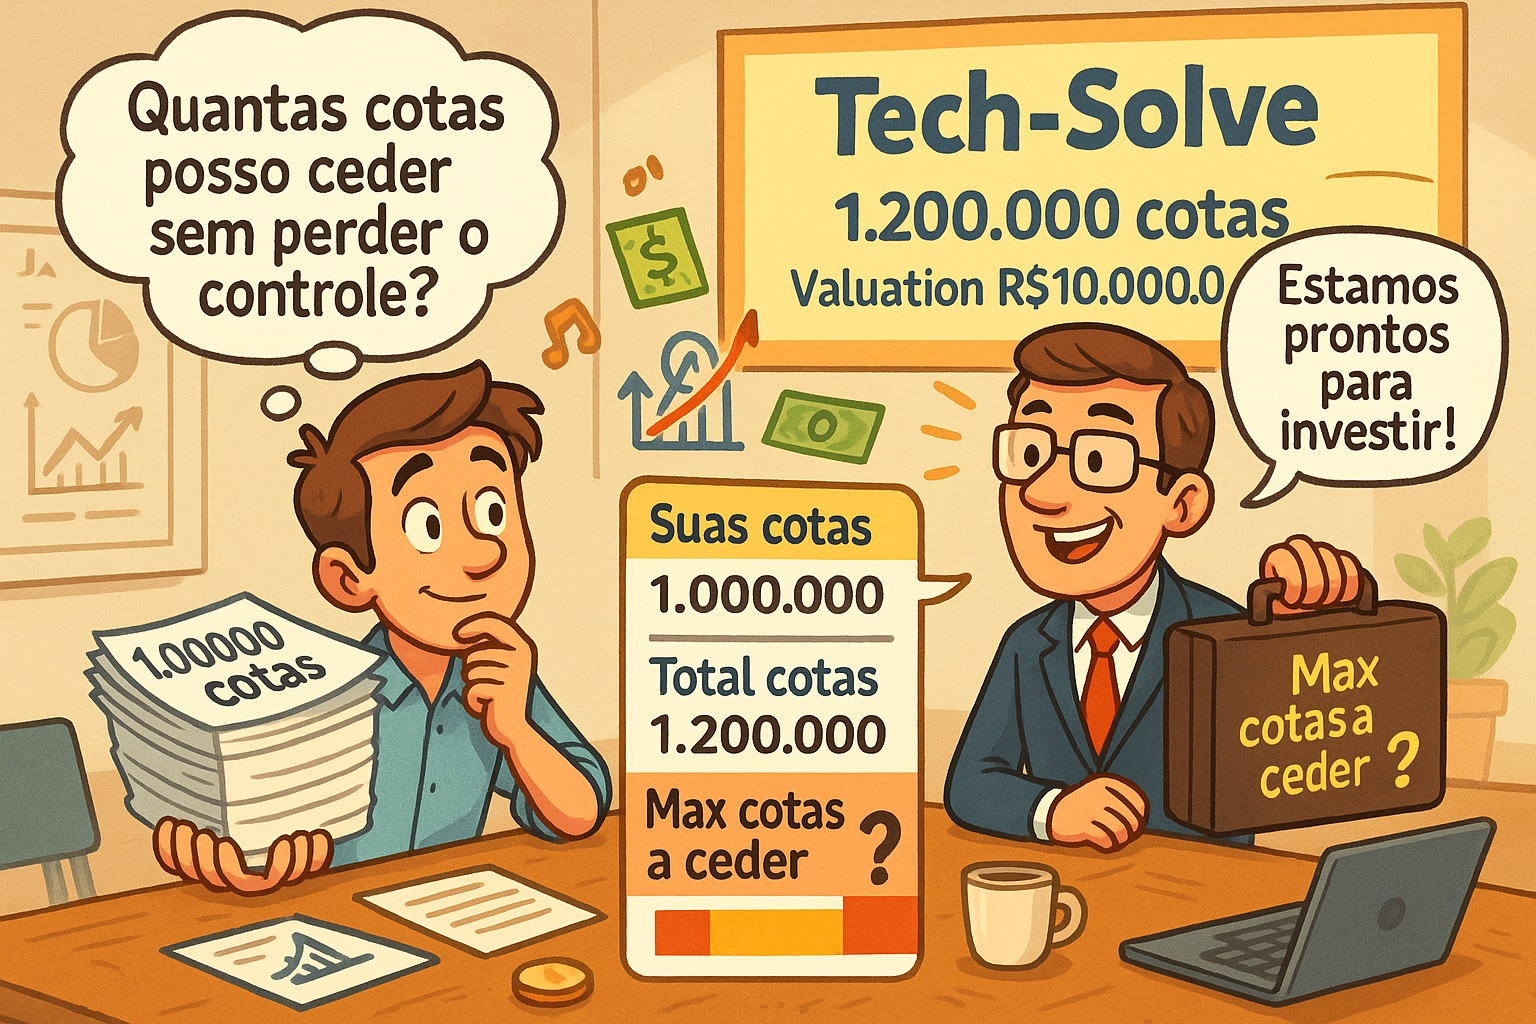
\includegraphics[width=7.03125in,height=\textheight]{images/03-2025-08-19_20/exercicio-02.jpg}

\begin{longtable}[]{@{}
  >{\raggedright\arraybackslash}p{(\columnwidth - 0\tabcolsep) * \real{1.0024}}@{}}
\toprule\noalign{}
\endhead
\bottomrule\noalign{}
\endlastfoot
Exercício 2 - Após o aporte inicial, sua startup ``Tech-Solve'' tem agora 1.200.000 cotas e um Capital Social (valuation) de R\$ 10.000.000. Você ainda detém 1.000.000 de cotas. Um fundo de Venture Capital se propõe a investir R\$ 3.000.000. Para que você mantenha o controle majoritário da empresa (mais de 51\% ou mais das cotas após o aporte), qual o número máximo de cotas que você pode ceder neste novo round? \\
\begin{minipage}[t]{\linewidth}\raggedright
\begin{enumerate}
\def\labelenumi{\alph{enumi})}
\tightlist
\item
  500.000 cotas
\end{enumerate}
\end{minipage} \\
\begin{minipage}[t]{\linewidth}\raggedright
\begin{enumerate}
\def\labelenumi{\alph{enumi})}
\setcounter{enumi}{1}
\tightlist
\item
  428.571 cotas
\end{enumerate}
\end{minipage} \\
\begin{minipage}[t]{\linewidth}\raggedright
\begin{enumerate}
\def\labelenumi{\alph{enumi})}
\setcounter{enumi}{2}
\tightlist
\item
  300.000 cotas
\end{enumerate}
\end{minipage} \\
\begin{minipage}[t]{\linewidth}\raggedright
\begin{enumerate}
\def\labelenumi{\alph{enumi})}
\setcounter{enumi}{3}
\tightlist
\item
  250.000 cotas
\end{enumerate}
\end{minipage} \\
\begin{minipage}[t]{\linewidth}\raggedright
\begin{enumerate}
\def\labelenumi{\alph{enumi})}
\setcounter{enumi}{4}
\tightlist
\item
  760.784 cotas
\end{enumerate}
\end{minipage} \\
\end{longtable}

\subsection{Resolução do Exercício II:}\label{resoluuxe7uxe3o-do-exercuxedcio-ii}

A empresa valorizou gerando valor por faturamento. Antes, eu e meu sócio-investidor tinhamos em caixa R\$ 6 milhões de CAPITAL SOCIAL.

Agora, após faturamento de produção e crescimento orgânico, o CAPITAL SOCIAL da empresa aumentou de R\$ 6 milhões para R\$ 10 milhões.

De toda forma, segundo o enunciado do exercício, eu continuo tendo 1.000.000 de cotas (83,333\% de participação no CAPITAL SOCIAL), enquanto que o outro sócio (sócio-investidor do exercício anterior) continua tendo 200.000 cotas (que representam os mesmos 16,67\% do capital social).

Como o CAPITAL SOCIAL aumentou de R\$ 6 milhões (total do exercício anterior) para R\$ 10 milhões agora, preciso saber quanto destes R\$ 10 mihões são a minha parte ( ``em reais'' ) e quanto é a parte do meu sócio investidor atualmente.

\[
\begin{array}{c|c}
\textbf{Quadro Societário}    & \textbf{Capital Social Original (R\$)} & \textbf{Capital Social Valorizado (R\$)} \\ 
\hline 
Sócio-FundadorOriginal        & 5.000.000,00 \quad (83,33\%) & ? \quad (83,33\%) \\
Sócio-Investidor-1            & 1.000.000,00 \quad (16,67\%) & ? \quad (16,67\%) \\
\hline
\textbf{Total} & 6.000.000,00 \quad (100\%) & 10.000.000,00 \quad (100\%)
\end{array}
\]

Vamos preencher a tabela

\[
\text{ 83,33% de R\$ 10.000.000,00 = R\$ 8.333.333,33} \\
\text{ 16,66% de R\$ 10.000.000,00 = R\$ 1.666.666,66}
\text{ } \\
\text{Portanto, a tabela de capital social atual da empresa é a seguinte: } \\
\text{ } \\
\begin{array}{c|c}
\textbf{Quadro Societário}    & \textbf{Capital Social Valorizado (R\$)} & \textbf{Cotas equivalentes} \\ 
\hline 
Sócio-FundadorOriginal        & 8.333.333,33 \quad (83,33\%) & 1.000.000 \\
Sócio-Investidor-1            & 1.666.666,66 \quad (16,67\%) & 200.000 \\
\hline
\textbf{Total}  & 10.000.000,00 \quad (100\%) & 1.200.000
\end{array}
\]

Agora temos um novo investidor, ou seja, candidato a terceiro sócio. Esse novo sócio quer investir R\$ 3.000.000,00 (três milhões de reais).

\[
\text{-----------------------------------------------} \\
\text{ CENÁRIO DA ENTRADA DO TERCEIRO SÓCIO:         } \\
\text{-----------------------------------------------} \\
\text{ } \\
\text{ ? % de R\$ 13.000.000,00 = R\$ 8.333.333,33} \\
\text{ ? % de R\$ 13.000.000,00 = R\$ 1.666.666,66} \\
\text{ ? % de R\$ 13.000.000,00 = R\$ 3.000.000,00} \\
\text{ } \\
\text{Portanto, a tabela de capital social atual da empresa é a seguinte: } \\
\text{ } \\
\begin{array}{c|c}
\textbf{Quadro Societário}    & \textbf{Capital Social Valorizado (R\$)} & \textbf{Cotas equivalentes} \\ 
\hline 
Sócio-FundadorOriginal        & 8.333.333,33 \quad (? \%) & 1.000.000 \\
Sócio-Investidor-1            & 1.666.666,66 \quad (? \%) & 200.000 \\
Sócio-Investidor-2            & 3.000.000,00 \quad (? \%) &  ? \\
\hline
\textbf{Total}  & 13.000.000,00 \quad (100\%) & ?
\end{array}
\]

Vamos descobrir qual a participação do novo sócio no capital social da empresa. Desta forma, em seguida, podemos descobrir quantas cotas iremos emitir para ele.

\[
\text{ ? % de R\$ 13.000.000,00 = R\$ 8.333.333,33} \\ 
\text{ ? % de R\$ 13.000.000,00 = R\$ 1.666.666,66} \\ 
\text{ ? % de R\$ 13.000.000,00 = R\$ 3.000.000,00} \\ 
\text{ } \\ 
\text{-----------------------------------------------} \\ 
\text{ REGRA DE 3:                                   } \\ 
\text{-----------------------------------------------} \\ 
\text{ } \\ 
\frac{13.000.000,00}{3.000.000,00} = \frac{100\%}{x\%} \\ 
x=\frac{[ (3.000.000,00) \times (100) ]}{13.000.000,00} \\ 
x=\frac{300.000.000,00}{13.000.000,00} \\ 
x= 23,07692 \% 
\text{ } \\ 
\text{ AGORA, SABENDO DA PARTICIPAÇÃO DO TERCEIRO SÓCIO, PODEMOS SABER QUANTAS COTAS DEVEMOS EMITIR PARA ELE } \\ 
\text{ } \\
\text{ TOTAL_COTAS_APOS_INVESTIMENTO } = \frac{ ( TOTAL\_COTAS\_ORIGINAIS )}{(100\% - PARTICIPACAO\_NOVO\_INVESTIDOR\%)} 
\text{ } \\ 
\text{TOTAL_COTAS_ORIGINAIS} \Rightarrow \quad \textbf{1.200.000} \quad \\ 
\text{ (um milhão duzentas mil cotas) } \\ 
\text{ } \\ 
\text{PARTICIPACAO_NOVO_INVESTIDOR } \quad \Rightarrow \quad \textbf{23,07692\%} \\ 
\text{ } \\ 
\text{TOTAL_COTAS_APOS_INVESTIMENTO} = \frac{1.200.000}{ (100\% - 23,07692\%} \\ 
\text{ } \\ 
\text{TOTAL_COTAS_APOS_INVESTIMENTO} = \frac{1.200.000}{ 1 - 0,2307692} \\ 
\text{ } \\ 
\text{TOTAL_COTAS_APOS_INVESTIMENTO} = \frac{1.200.000}{ 0,7692308} \\ 
\text{ } \\ 
\text{TOTAL_COTAS_APOS_INVESTIMENTO} = \text{1.560.000 quotas} \\ 
\text{ } \\ 
\text{ Cotas ao novo investidor } = \text{Total de Cotas atuais - Total de cotas anteriores} \\ 
\text{ } \\ 
\text{ Cotas ao novo investidor } = \text{ 1.560.000 - 1.200.000 } \\ 
\text{ } \\ 
\text{ Cotas ao novo investidor } = \textbf{ 360.000 } \text{cotas.}
\text{ } \\
\text{ } \\ 
\begin{array}{c|c}
\textbf{Quadro Societário}    & \textbf{Capital Social  (R\$)} & \textbf{Cotas equivalentes} \\ 
\hline 
Sócio-FundadorOriginal        & 8.333.333,33 \quad (64,1025 \%) & 1.000.000 \\
Sócio-Investidor-1            & 1.666.666,66 \quad (12,8205 \%) & 200.000 \\
Sócio-Investidor-2            & 3.000.000,00 \quad (23,0769 \%) & 360.000 \\
\hline
\textbf{Total}  & 13.000.000,00 \quad (100\%) & 1.560.000
\end{array}
\]

E para finalizar, a pergunta do exercício:

\[
\text{ O INVESTIDOR ORIGINAL SÓ PERDE A MAJORIDADE SE FICAR COM MENOS DE 51\% DO CAPITAL SOCIAL} \\ 
\text{ } \\ \text{ COMO VIMOS neste EXERCÍCIO, ELE POSSUI R\$ 8.333.333,33 MILHÕES DE PARTICIPAÇÃO NO CAPITAL SOCIAL } \\ 
\text{ } \\ \text{ APÓS O NOVO SÓCIO TER INVESTIDO 3 MILHÃO, A EMPRESA PASSOU A TER 13 MILHÕES DE CAPITAL SOCIAL } \\ 
\text{ } \\ 
\text{ SENDO QUE DESTES 13 MILHÕES, R\$ 8.333.333,33 MILHÕES SÃO DO ANTIGO DONO (R\$ 8.333.333,33 MILHÕES REPRESENTAM 64,1025\% DO VALOR TOTAL) } \\ 
\text{ } \\ 
\\text{ A PERGUNTA AGORA SERIA: "QUAL VALOR TOTAL ONDE 5 MILHÕES REPRESENTAM 51\% DELE") } \\ 
\text{ } \\ \text{ VAMOS UTILIZAR NOVAMENTE A REGRA DE 3} \\ 
\text{ } \\ \qquad\frac{ x }{ 8.333.333,33 }= \frac{ 100 \% }{51 \%} \qquad \Rightarrow \qquad \frac{ [ ( x ) \times (51) ] }{ [ ( R\$ 8.333.333,33 ) \times (100) ] } \\ 
51*x = (R\$ 8.333.333,33 )* \times (100) \\ 
51x = (R\$ 8.333.333,33) \\ 
\text{ } \\ 
x=\frac{ 833.333.333,00 }{51} \\ 
\text{ } \\ 
x= 16.339.869,27451 \\ 
\text{ R\$ 16.339.869,27451 é o valor total de dinheiro em caixa onde R\$ 8.333.333,33 representam 51\% deste valor } \\ 
\text{ } \\ 
\text{ Assim, sabendo que já tinhamos R\$ 10.000.000,00 em caixa, se o investidor investisse mais R\$ 6.339.869,27451 } \\ 
\text{ o total em caixa chegava a R\$ 16.339.869,27451 DE CAPITAL SOCIAL , quantidade máxima de capital social total para que os 5 milhões do antigo dono } \\ 
\text{ representassem 51\% da participação na sociedade. } \\ 
\text{ Um investidor pode investir no máximo } \textbf{R\$ R\$ 6.339.869,27451 } \text{ para que o antigo dono ainda seja mandatário na empresa } \\ 
\text{ } \\
\]

Quantas cotas esse ivestimento de R\$ 6.339.869,27451 produziria ao novo investidor ?

\[ 
\text{-----------------------------------------------} \\ 
\text{ REGRA DE 3:                                   } \\ 
\text{-----------------------------------------------} \\ 
\text{ } \\ 
\frac{16.339.869,27}{6.339.869,27} = \frac{100\%}{x\%} \\ 
x=\frac{[ (6.339.869,27) \times (100) ]}{16.339.869,27} \\ 
x=\frac{633.986.927}{16.339.869,27} \\ 
x= 38,80 \% \text{ } \\ 
\text{ } \\
\text{ AGORA, SABENDO DA PARTICIPAÇÃO HIPOTÉTICA DO TERCEIRO SÓCIO, PODEMOS SABER QUANTAS COTAS DEVEMOS EMITIR PARA ELE } \\ 
\text{ } \\ 
\text{ TOTAL_COTAS_APOS_INVESTIMENTO } = \frac{ ( TOTAL\_COTAS\_ORIGINAIS )}{(100\% - PARTICIPACAO\_NOVO\_INVESTIDOR\%)}  \\
\text{ } \\ \text{ TOTAL_COTAS_APOS_INVESTIMENTO } = \frac{ ( 1.200.000 )}{(100\% - 38,8\%)} \\ 
\text{ } \\ \text{ TOTAL_COTAS_APOS_INVESTIMENTO } = \frac{ ( 1.200.000 )}{(100\% - 38,8\%)} \\ 
\text{ TOTAL_COTAS_APOS_INVESTIMENTO } = \frac{ ( 1.200.000 )}{(0,61)} \\ 
\text{ TOTAL_COTAS_APOS_INVESTIMENTO } = 1.960.784 \\ 
\text{ Cotas máximas a emitir sem o sócio-fundados perder os 51\% } = [(1.960.784 ) - (1.200.000)] \\ 
\text{ Cotas máximas a emitir sem o sócio-fundados perder os 51\% } = 760.784 \quad \text{cotas} 
\]

\subsection{\texorpdfstring{\textbf{Exercício 3:} Aporte Growth Capital (Série B)}{Exercício 3: Aporte Growth Capital (Série B)}}\label{exercuxedcio-3-aporte-growth-capital-suxe9rie-b}

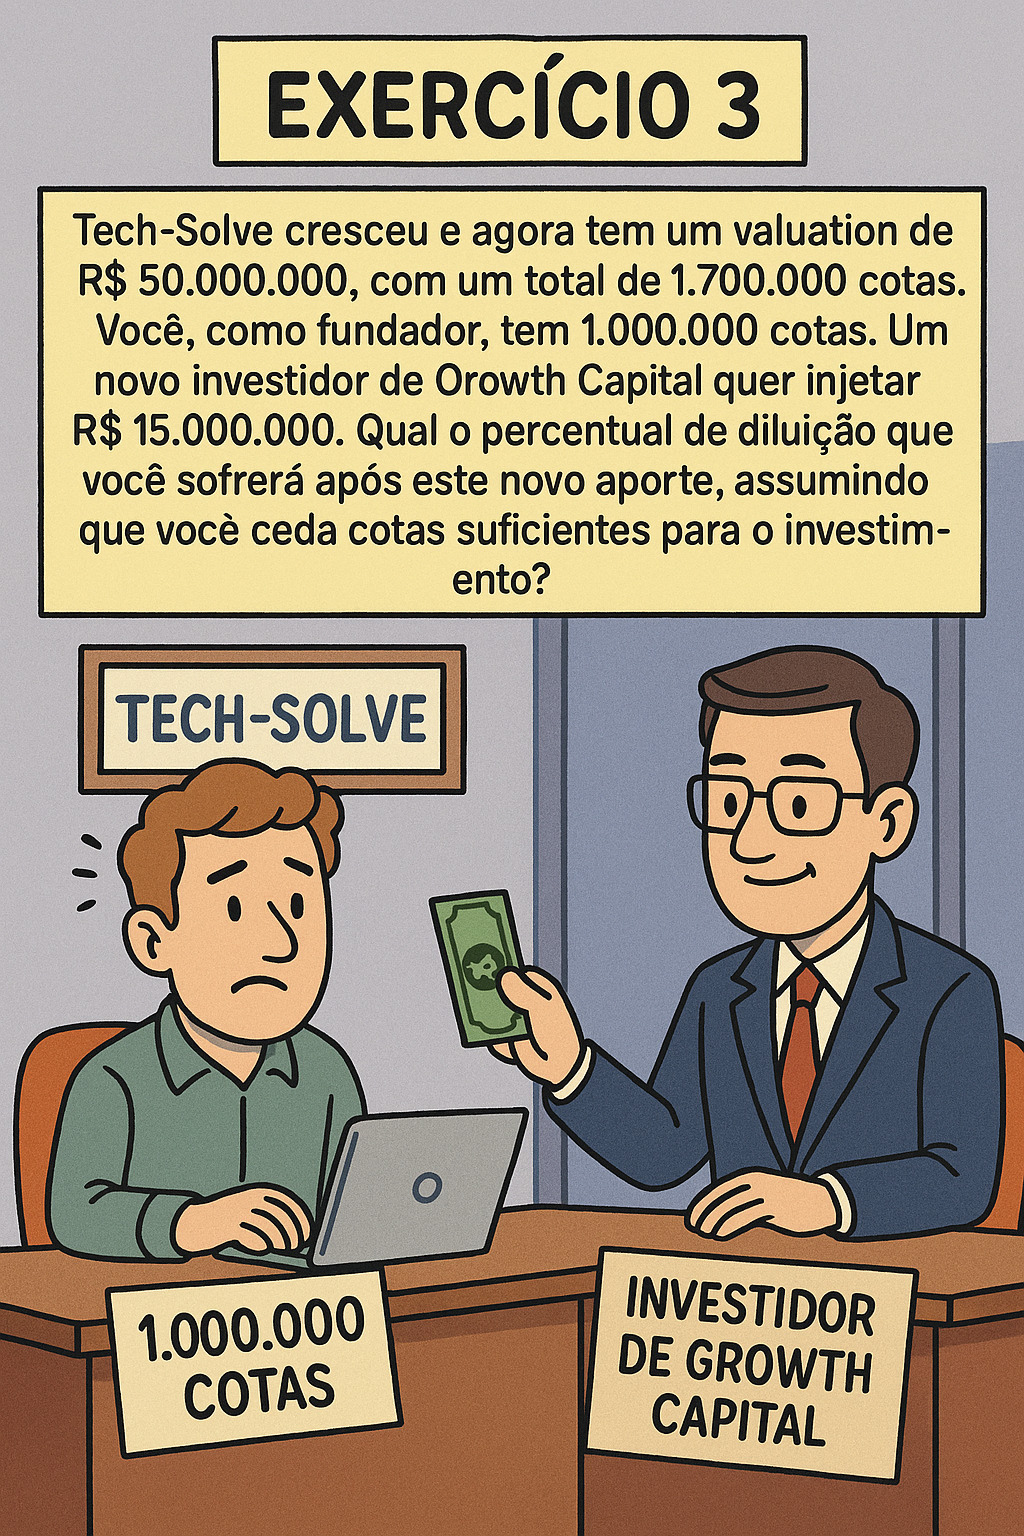
\includegraphics[width=4.20833in,height=\textheight]{images/03-2025-08-19_20/exercicio-03.jpg}

\begin{longtable}[]{@{}
  >{\raggedright\arraybackslash}p{(\columnwidth - 0\tabcolsep) * \real{1.0028}}@{}}
\toprule\noalign{}
\endhead
\bottomrule\noalign{}
\endlastfoot
Exercício 3 - ``Tech-Solve'' cresceu e agora tem um valuation de R\$ 50.000.000, com um total de 1.700.000 cotas. Você, como fundador, tem 1.000.000 cotas. Um novo investidor de Growth Capital quer injetar R\$ 15.000.000. Qual o percentual de diluição que você sofrerá após este novo aporte, assumindo que você ceda cotas suficientes para o investimento? \\
\begin{minipage}[t]{\linewidth}\raggedright
\begin{enumerate}
\def\labelenumi{\alph{enumi})}
\tightlist
\item
  23,08\%
\end{enumerate}
\end{minipage} \\
\begin{minipage}[t]{\linewidth}\raggedright
\begin{enumerate}
\def\labelenumi{\alph{enumi})}
\setcounter{enumi}{1}
\tightlist
\item
  18,75\%
\end{enumerate}
\end{minipage} \\
\begin{minipage}[t]{\linewidth}\raggedright
\begin{enumerate}
\def\labelenumi{\alph{enumi})}
\setcounter{enumi}{2}
\tightlist
\item
  20,00\%
\end{enumerate}
\end{minipage} \\
\begin{minipage}[t]{\linewidth}\raggedright
\begin{enumerate}
\def\labelenumi{\alph{enumi})}
\setcounter{enumi}{3}
\tightlist
\item
  25,00\%
\end{enumerate}
\end{minipage} \\
\end{longtable}

\subsection{Exercício 4: Cenário de Múltiplos Investidores}\label{exercuxedcio-4-cenuxe1rio-de-muxfaltiplos-investidores}

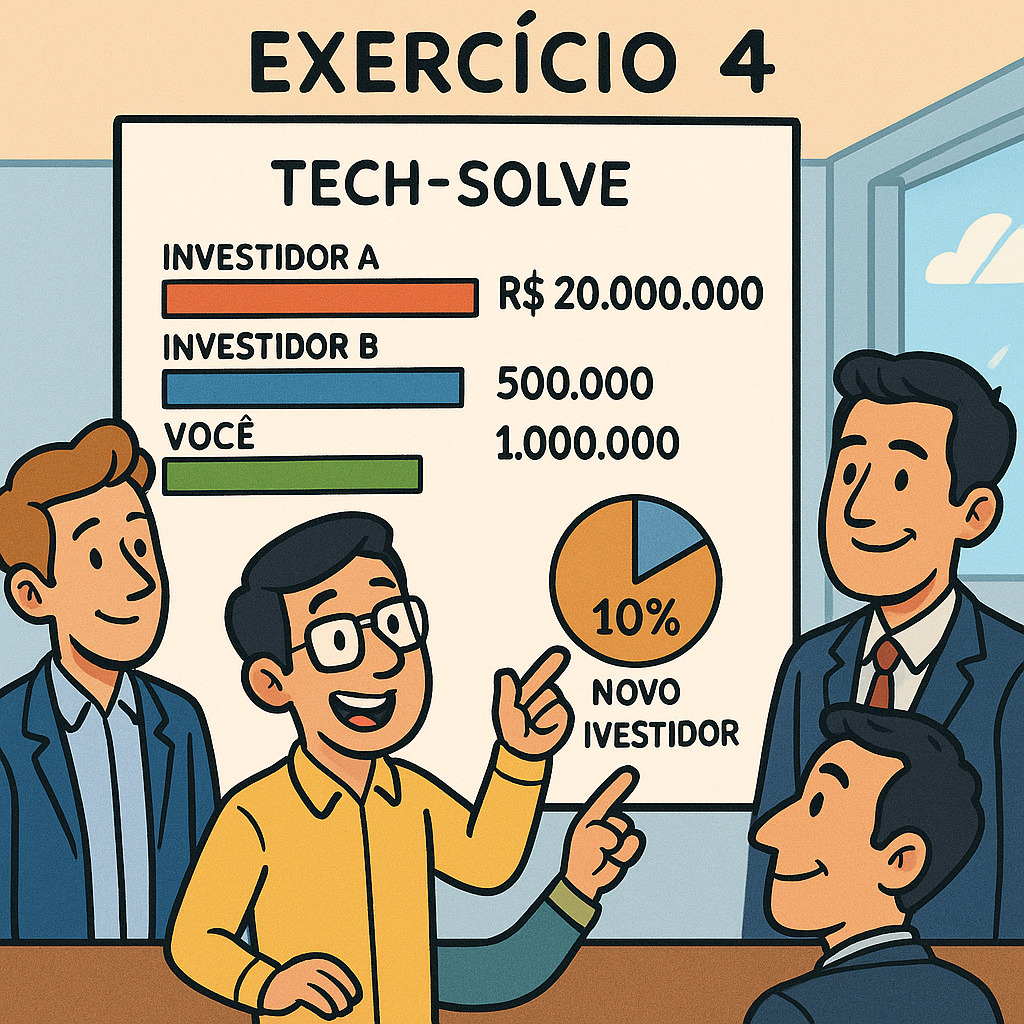
\includegraphics[width=7.15625in,height=\textheight]{images/03-2025-08-19_20/exercicio-04.jpg}

\begin{longtable}[]{@{}
  >{\raggedright\arraybackslash}p{(\columnwidth - 0\tabcolsep) * \real{1.0028}}@{}}
\toprule\noalign{}
\endhead
\bottomrule\noalign{}
\endlastfoot
Exercício 4 - ``Tech-Solve'' agora tem 1.000.000 de cotas originais, um investidor A com 200.000 cotas e um investidor B com 500.000 cotas. Sua participação é de 1.000.000 de cotas. A empresa está avaliada em R\$ 20.000.000. Um novo investidor quer comprar 10\% da empresa. Quantas cotas ele deve receber, e qual será sua nova participação percentual na empresa? \\
\begin{minipage}[t]{\linewidth}\raggedright
\begin{enumerate}
\def\labelenumi{\alph{enumi})}
\tightlist
\item
  150.000 cotas; 8,8\%
\end{enumerate}
\end{minipage} \\
\begin{minipage}[t]{\linewidth}\raggedright
\begin{enumerate}
\def\labelenumi{\alph{enumi})}
\setcounter{enumi}{1}
\tightlist
\item
  200.000 cotas; 10,0\%
\end{enumerate}
\end{minipage} \\
\begin{minipage}[t]{\linewidth}\raggedright
\begin{enumerate}
\def\labelenumi{\alph{enumi})}
\setcounter{enumi}{2}
\tightlist
\item
  190.000 cotas; 9,5\%
\end{enumerate}
\end{minipage} \\
\begin{minipage}[t]{\linewidth}\raggedright
\begin{enumerate}
\def\labelenumi{\alph{enumi})}
\setcounter{enumi}{3}
\tightlist
\item
  170.000 cotas; 8,5\%
\end{enumerate}
\end{minipage} \\
\end{longtable}

\subsection{Exercício 5: Protegendo a Maioria}\label{exercuxedcio-5-protegendo-a-maioria}

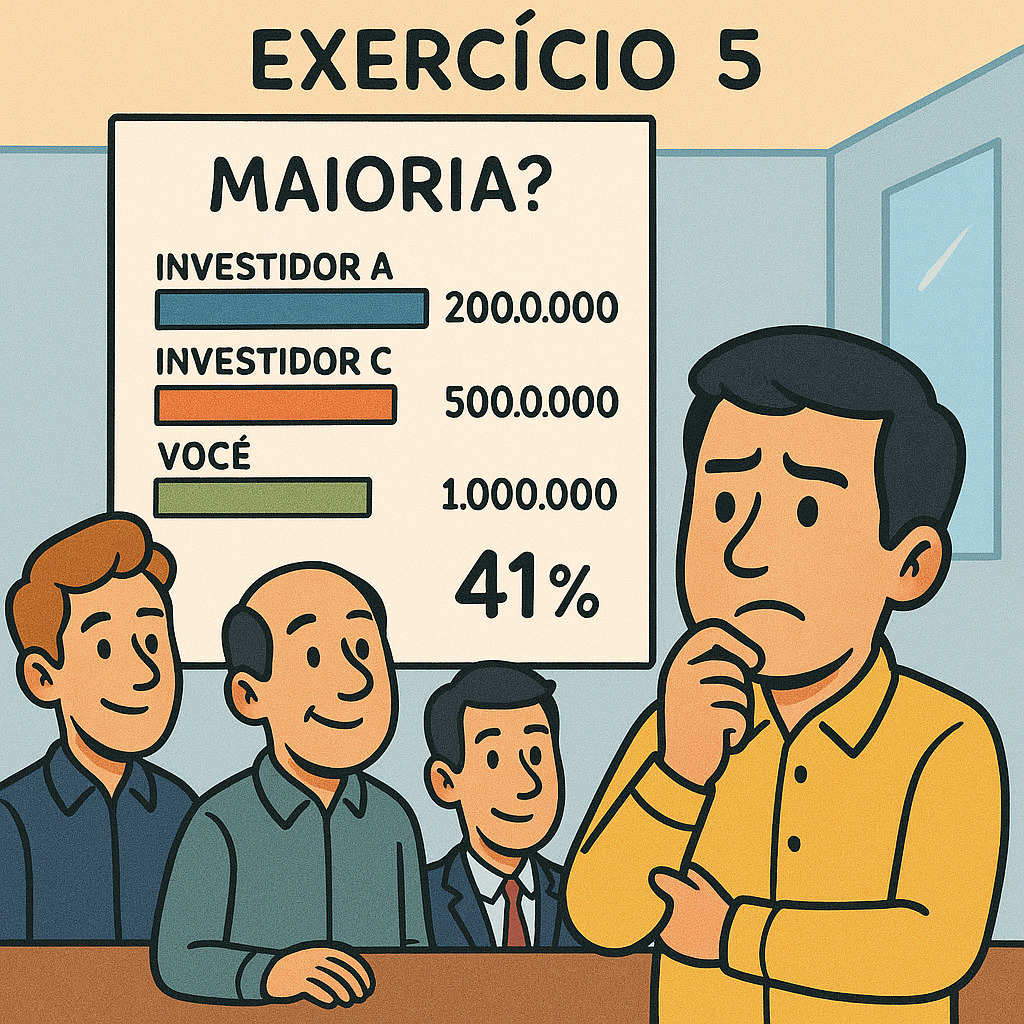
\includegraphics[width=6.94792in,height=\textheight]{images/03-2025-08-19_20/exercicio-05.jpg}

\begin{longtable}[]{@{}
  >{\raggedright\arraybackslash}p{(\columnwidth - 0\tabcolsep) * \real{1.0026}}@{}}
\toprule\noalign{}
\endhead
\bottomrule\noalign{}
\endlastfoot
Exercício 5 - Considere que, após todos os aportes (do Exercício 1 ao 4), você ainda deseja manter o controle majoritário da sua startup. O investidor A tem 200.000 cotas e o investidor B tem 500.000 cotas. No último aporte, o investidor C recebeu 190.000 cotas. Você começou com 1.000.000 de cotas. Qual a sua participação percentual atual na empresa, e você ainda tem a maioria? \\
\begin{minipage}[t]{\linewidth}\raggedright
\begin{enumerate}
\def\labelenumi{\alph{enumi})}
\tightlist
\item
  50,0\% - Não tem a maioria
\end{enumerate}
\end{minipage} \\
\begin{minipage}[t]{\linewidth}\raggedright
\begin{enumerate}
\def\labelenumi{\alph{enumi})}
\setcounter{enumi}{1}
\tightlist
\item
  51,5\% - Tem a maioria
\end{enumerate}
\end{minipage} \\
\begin{minipage}[t]{\linewidth}\raggedright
\begin{enumerate}
\def\labelenumi{\alph{enumi})}
\setcounter{enumi}{2}
\tightlist
\item
  48,0\% - Não tem a maioria
\end{enumerate}
\end{minipage} \\
\begin{minipage}[t]{\linewidth}\raggedright
\begin{enumerate}
\def\labelenumi{\alph{enumi})}
\setcounter{enumi}{3}
\tightlist
\item
  49,5\% - Não tem a maioria
\end{enumerate}
\end{minipage} \\
\end{longtable}

\section{Respostas dos exercícios}\label{respostas-dos-exercuxedcios-1}

\begin{longtable}[]{@{}ll@{}}
\toprule\noalign{}
\endhead
\bottomrule\noalign{}
\endlastfoot
Exercício & Resposta \\
1 Modelo & b \\
2 & c \\
3 & a \\
4 & c \\
5 & b \\
\end{longtable}

\section{Referências}\label{referuxeancias-1}

ROSSETTI, José Paschoal; ANDRADE, Adriana. \emph{Governança Corporativa: Fundamentos, Desenvolvimento e Tendências}. São Paulo: Atlas, 7. ed., 2014. p.~s.p.

SILVEIRA, Alexandre Di Miceli da. \emph{Governança Corporativa no Brasil e no Mundo: Teoria e Prática}. Rio de Janeiro: Elsevier, 2010.

\chapter{Governança Corporativa - Conselhos da Empresa}\label{governanuxe7a-corporativa---conselhos-da-empresa}

\subsubsection*{26/08/2025 - Campus Marquês}\label{campus-marquuxeas-3}
\addcontentsline{toc}{subsubsection}{26/08/2025 - Campus Marquês}

\subsubsection*{27/08/2025 - Campus Chácara}\label{campus-chuxe1cara-3}
\addcontentsline{toc}{subsubsection}{27/08/2025 - Campus Chácara}

\section{Fisiologia da Governança Corporativa --}\label{fisiologia-da-governanuxe7a-corporativa}

\subsection{Conselho de Administração}\label{conselho-de-administrauxe7uxe3o}

\begin{quote}
O \textbf{Conselho de Administração} é o órgão de orientação estratégica de uma empresa com governança corporativa.
\end{quote}

\begin{center}\rule{0.5\linewidth}{0.5pt}\end{center}

\subsubsection{Competências do Conselho de Administração}\label{competuxeancias-do-conselho-de-administrauxe7uxe3o}

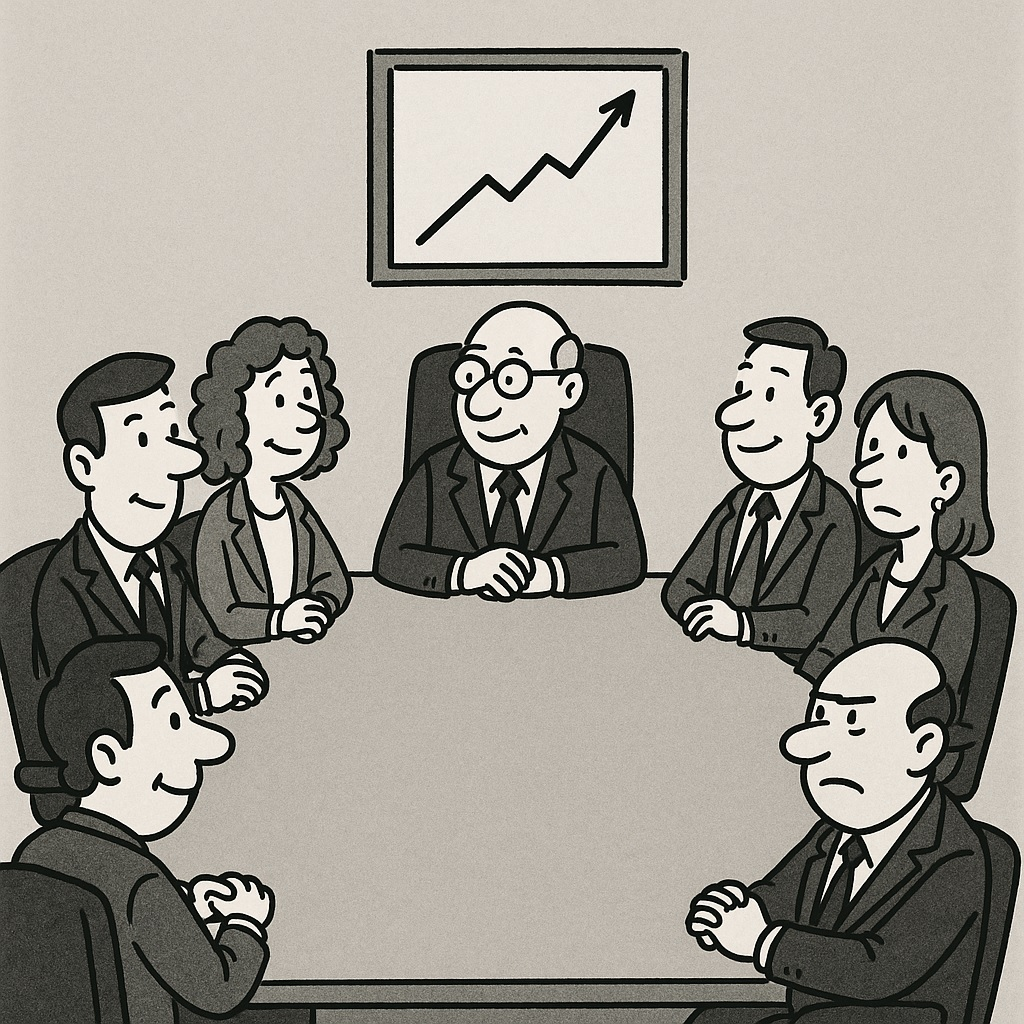
\includegraphics{images/04-2025-08-26_27/01-conselho_administrativo.jpg}

\begin{itemize}
\tightlist
\item
  Definição da estratégia da empresa\\
\item
  Eleição e destituição do seu principal executivo\\
\item
  Aprovação da escolha ou da dispensa dos demais executivos sob proposta do executivo principal (CEO)\\
\item
  Acompanhamento da gestão\\
\item
  Monitoramento dos riscos\\
\item
  Indicação e substituição dos auditores independentes
\end{itemize}

\begin{center}\rule{0.5\linewidth}{0.5pt}\end{center}

\subsubsection{Boa Prática}\label{boa-pruxe1tica}

Atualmente, é considerada uma boa prática a formação do Conselho de Administração com o maior número possível de \textbf{conselheiros independentes}.

\begin{center}\rule{0.5\linewidth}{0.5pt}\end{center}

\subsection{Conselho Fiscal}\label{conselho-fiscal}

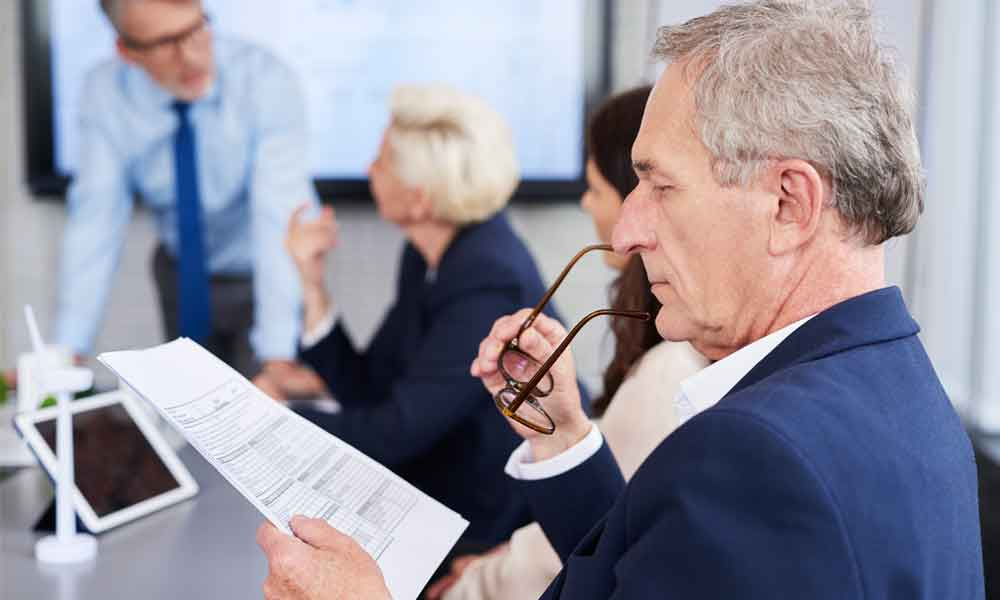
\includegraphics[width=5.15625in,height=\textheight]{images/04-2025-08-26_27/02-conselho_fiscal.jpg}

\begin{quote}
O \textbf{Conselho Fiscal} é o órgão de fiscalização dos acionistas/cotistas.
\end{quote}

\subsubsection{Competências do Conselho Fiscal}\label{competuxeancias-do-conselho-fiscal}

\begin{itemize}
\tightlist
\item
  é um órgão \textbf{não obrigatório};
\item
  tem como objetivo \textbf{fiscalizar os atos da administração}, verificar o \emph{compliance} e dar informações seguras aos sócios;
\item
  atua como um \textbf{controle independente} para os sócios; e
\item
  deve ser visto como um órgão que possui instrumentos que visam \textbf{agregar valor à sociedade}.
\end{itemize}

\begin{center}\rule{0.5\linewidth}{0.5pt}\end{center}

\subsection{Conselho Consultivo}\label{conselho-consultivo}

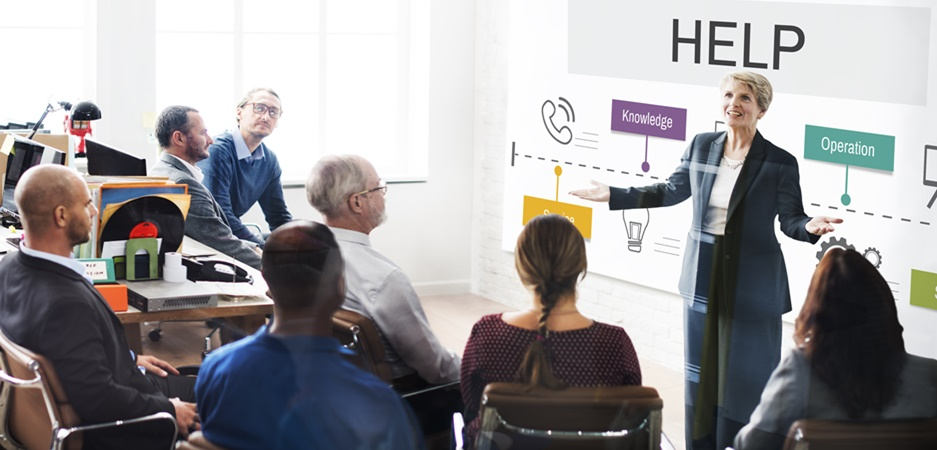
\includegraphics[width=8.30208in,height=\textheight]{images/04-2025-08-26_27/03-conselho_consultivo.jpg}

\begin{itemize}
\tightlist
\item
  Órgão \textbf{não deliberativo}, mas que dá suporte às decisões do Conselho de Administração.
\item
  Recomendado para empresas cujo Conselho de Administração seja formado por conselheiros \textbf{acionistas/cotistas} (portanto, não independentes) e que necessitem de \textbf{competências técnicas} para amparar as suas decisões.
\item
  Indicado também para empresas que estejam na \textbf{fase inicial de implantação} de uma arquitetura de governança corporativa.
\end{itemize}

\begin{center}\rule{0.5\linewidth}{0.5pt}\end{center}

\section{ESTUDO DE CASO: SAÍDA DE STEEVE JOBS DA APPLE}\label{estudo-de-caso-sauxedda-de-steeve-jobs-da-apple}

\begin{longtable}[]{@{}
  >{\raggedright\arraybackslash}p{(\columnwidth - 4\tabcolsep) * \real{0.2733}}
  >{\raggedright\arraybackslash}p{(\columnwidth - 4\tabcolsep) * \real{0.3230}}
  >{\raggedright\arraybackslash}p{(\columnwidth - 4\tabcolsep) * \real{0.3975}}@{}}
\toprule\noalign{}
\begin{minipage}[b]{\linewidth}\raggedright
Acionista-Fundador gestor (minoritário)

Steeve Jobs
\end{minipage} & \begin{minipage}[b]{\linewidth}\raggedright
CEO

John Sculley
\end{minipage} & \begin{minipage}[b]{\linewidth}\raggedright
Acionista Majoritário

Arthur Rock
\end{minipage} \\
\midrule\noalign{}
\endhead
\bottomrule\noalign{}
\endlastfoot
\includegraphics{images/04-2025-08-26_27/10-jobs.webp} & 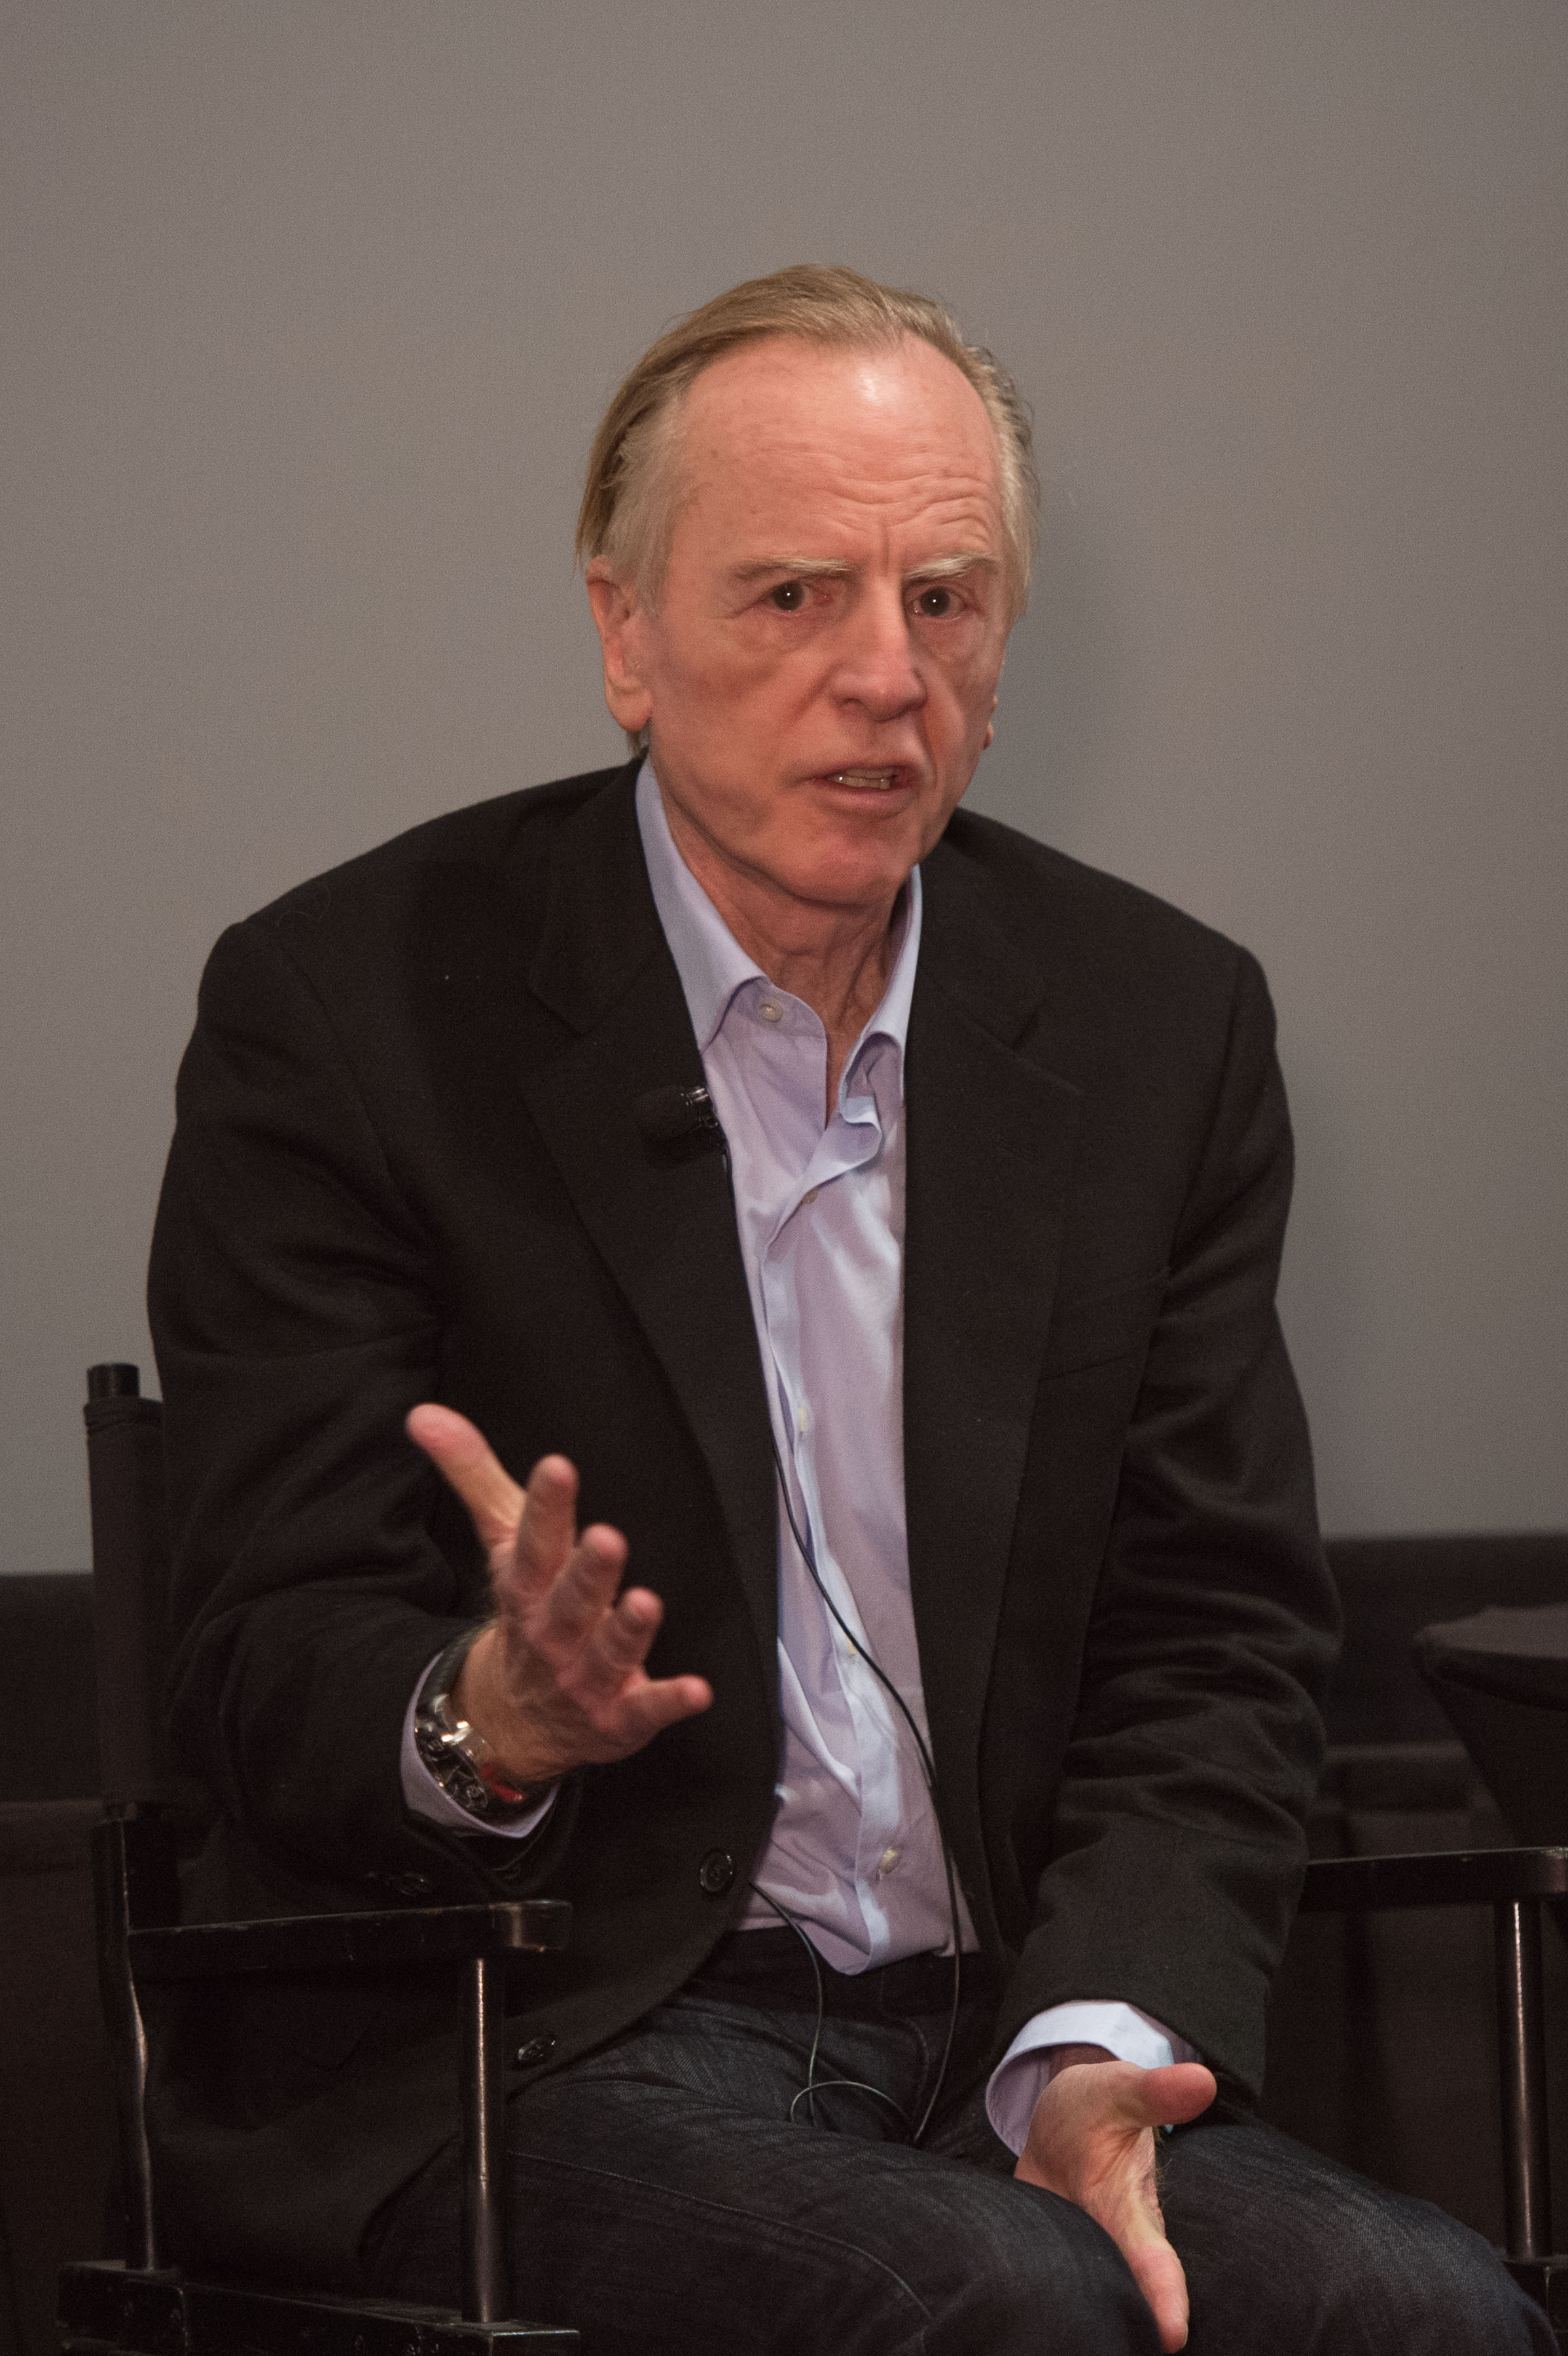
\includegraphics{images/04-2025-08-26_27/John_Sculley_III.jpg} & 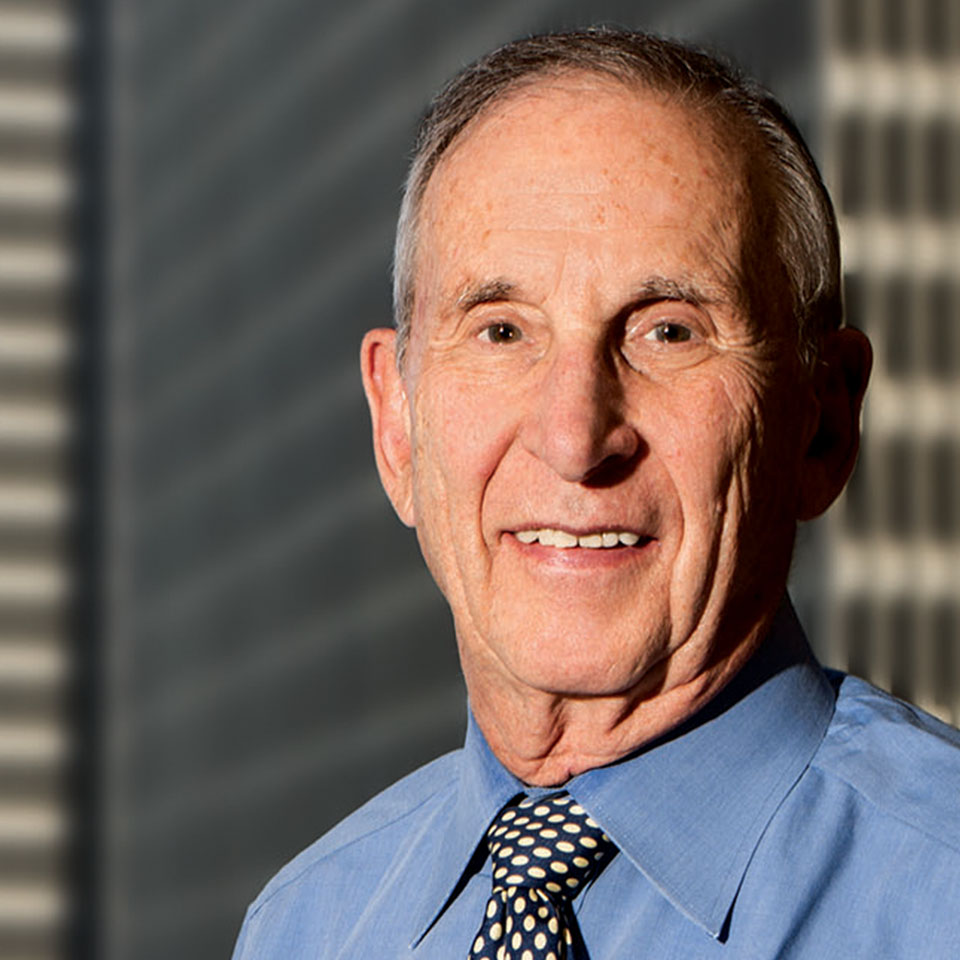
\includegraphics[width=3.20833in,height=\textheight]{images/04-2025-08-26_27/Rock_Arthur_960.jpg} \\
\end{longtable}

\subsection{Linha do Tempo: Steve Jobs e a Apple (1976--1997)}\label{linha-do-tempo-steve-jobs-e-a-apple-19761997}

\subsubsection{- 1976 -- Steve Jobs e Steve Wozniak fundam a Apple Computer na garagem da família Jobs, em Cupertino.}\label{steve-jobs-e-steve-wozniak-fundam-a-apple-computer-na-garagem-da-famuxedlia-jobs-em-cupertino.}

\subsubsection{- 1977 -- Lançamento do Apple II, primeiro grande sucesso comercial.}\label{lanuxe7amento-do-apple-ii-primeiro-grande-sucesso-comercial.}

\subsubsection{- 1980 -- A Apple abre seu capital na bolsa (IPO), valorizando fortemente a empresa.}\label{a-apple-abre-seu-capital-na-bolsa-ipo-valorizando-fortemente-a-empresa.}

\subsubsection{- 1983 -- Jobs convence John Sculley, então CEO da PepsiCo, a assumir como CEO da Apple com a famosa frase:}\label{jobs-convence-john-sculley-entuxe3o-ceo-da-pepsico-a-assumir-como-ceo-da-apple-com-a-famosa-frase}

``Você quer vender água com açúcar pelo resto da sua vida ou quer mudar o mundo comigo?''

\subsubsection{- 1984 -- Lançamento do Macintosh, com a campanha icônica no Super Bowl.}\label{lanuxe7amento-do-macintosh-com-a-campanha-icuxf4nica-no-super-bowl.}

\subsubsection{- 1985 -- Conflito entre Steve Jobs e John Sculley sobre o rumo da empresa.}\label{conflito-entre-steve-jobs-e-john-sculley-sobre-o-rumo-da-empresa.}

Jobs perde apoio da diretoria, liderada por Arthur Rock (investidor e presidente do board).

Resultado: Steve Jobs é afastado da Apple.

\subsubsection{- 1985--1996 -- Período fora da Apple:}\label{peruxedodo-fora-da-apple}

Jobs funda a NeXT Computer.

Adquire e transforma a Pixar Animation Studios, que em 1995 lança Toy Story, primeiro longa em animação digital.

\subsubsection{- 1996 -- A Apple compra a NeXT por US\$ 429 milhões para obter seu sistema operacional (base do futuro macOS).}\label{a-apple-compra-a-next-por-us-429-milhuxf5es-para-obter-seu-sistema-operacional-base-do-futuro-macos.}

\subsubsection{- 1997 -- Steve Jobs retorna à Apple como conselheiro e, pouco depois, CEO interino (``iCEO'').}\label{steve-jobs-retorna-uxe0-apple-como-conselheiro-e-pouco-depois-ceo-interino-iceo.}

Início do processo de revitalização que levaria ao

\subsubsection{- iMac (1998)}\label{imac-1998}

\subsubsection{- iPod (2001)}\label{ipod-2001}

\subsubsection{- iPhone (2007)}\label{iphone-2007}

\subsubsection{- iPad (2010)}\label{ipad-2010}

\section{Exercícios}\label{exercuxedcios-2}

\begin{center}\rule{0.5\linewidth}{0.5pt}\end{center}

\begin{longtable}[]{@{}
  >{\raggedright\arraybackslash}p{(\columnwidth - 0\tabcolsep) * \real{1.0127}}@{}}
\toprule\noalign{}
\begin{minipage}[b]{\linewidth}\raggedright
\textbf{Exercício 1:}
\end{minipage} \\
\midrule\noalign{}
\endhead
\bottomrule\noalign{}
\endlastfoot
\textbf{Qual das seguintes competências é atribuída ao Conselho de Administração?} \\
\begin{minipage}[t]{\linewidth}\raggedright
\begin{enumerate}
\def\labelenumi{\alph{enumi})}
\tightlist
\item
  Executar as operações diárias da empresa.
\end{enumerate}
\end{minipage} \\
\begin{minipage}[t]{\linewidth}\raggedright
\begin{enumerate}
\def\labelenumi{\alph{enumi})}
\setcounter{enumi}{1}
\tightlist
\item
  Definir a estratégia da empresa.
\end{enumerate}
\end{minipage} \\
\begin{minipage}[t]{\linewidth}\raggedright
\begin{enumerate}
\def\labelenumi{\alph{enumi})}
\setcounter{enumi}{2}
\tightlist
\item
  Realizar auditorias financeiras internas detalhadas.
\end{enumerate}
\end{minipage} \\
\begin{minipage}[t]{\linewidth}\raggedright
\begin{enumerate}
\def\labelenumi{\alph{enumi})}
\setcounter{enumi}{3}
\tightlist
\item
  Gerenciar o fluxo de caixa da empresa diretamente.
\end{enumerate}
\end{minipage} \\
\begin{minipage}[t]{\linewidth}\raggedright
\begin{enumerate}
\def\labelenumi{\alph{enumi})}
\setcounter{enumi}{4}
\tightlist
\item
  Aprovar campanhas de marketing sem proposta do CEO.
\end{enumerate}
\end{minipage} \\
\end{longtable}

\begin{center}\rule{0.5\linewidth}{0.5pt}\end{center}

\begin{longtable}[]{@{}
  >{\raggedright\arraybackslash}p{(\columnwidth - 0\tabcolsep) * \real{1.0074}}@{}}
\toprule\noalign{}
\begin{minipage}[b]{\linewidth}\raggedright
\textbf{Exercício 2:}
\end{minipage} \\
\midrule\noalign{}
\endhead
\bottomrule\noalign{}
\endlastfoot
\textbf{De acordo com os documentos, qual é a principal definição do Conselho de Administração em uma empresa com governança corporativa?} \\
\begin{minipage}[t]{\linewidth}\raggedright
\begin{enumerate}
\def\labelenumi{\alph{enumi})}
\tightlist
\item
  É o órgão de fiscalização dos acionistas/cotistas.
\end{enumerate}
\end{minipage} \\
\begin{minipage}[t]{\linewidth}\raggedright
\begin{enumerate}
\def\labelenumi{\alph{enumi})}
\setcounter{enumi}{1}
\tightlist
\item
  É responsável pela gestão operacional e tática da empresa.
\end{enumerate}
\end{minipage} \\
\begin{minipage}[t]{\linewidth}\raggedright
\begin{enumerate}
\def\labelenumi{\alph{enumi})}
\setcounter{enumi}{2}
\tightlist
\item
  É o órgão de orientação estratégica de uma empresa.
\end{enumerate}
\end{minipage} \\
\begin{minipage}[t]{\linewidth}\raggedright
\begin{enumerate}
\def\labelenumi{\alph{enumi})}
\setcounter{enumi}{3}
\tightlist
\item
  Fornece suporte técnico não deliberativo às decisões executivas.
\end{enumerate}
\end{minipage} \\
\begin{minipage}[t]{\linewidth}\raggedright
\begin{enumerate}
\def\labelenumi{\alph{enumi})}
\setcounter{enumi}{4}
\tightlist
\item
  Implementa a estratégia definida pelos acionistas minoritários.
\end{enumerate}
\end{minipage} \\
\end{longtable}

\begin{center}\rule{0.5\linewidth}{0.5pt}\end{center}

\begin{longtable}[]{@{}
  >{\raggedright\arraybackslash}p{(\columnwidth - 0\tabcolsep) * \real{1.0127}}@{}}
\toprule\noalign{}
\begin{minipage}[b]{\linewidth}\raggedright
\textbf{Exercício 3:}
\end{minipage} \\
\midrule\noalign{}
\endhead
\bottomrule\noalign{}
\endlastfoot
\textbf{Uma boa prática atual para a formação do Conselho de Administração é que:} \\
\begin{minipage}[t]{\linewidth}\raggedright
\begin{enumerate}
\def\labelenumi{\alph{enumi})}
\tightlist
\item
  Seja formado exclusivamente por executivos da própria empresa.
\end{enumerate}
\end{minipage} \\
\begin{minipage}[t]{\linewidth}\raggedright
\begin{enumerate}
\def\labelenumi{\alph{enumi})}
\setcounter{enumi}{1}
\tightlist
\item
  Tenha o menor número possível de conselheiros independentes.
\end{enumerate}
\end{minipage} \\
\begin{minipage}[t]{\linewidth}\raggedright
\begin{enumerate}
\def\labelenumi{\alph{enumi})}
\setcounter{enumi}{2}
\tightlist
\item
  O maior número possível de conselheiros seja independente.
\end{enumerate}
\end{minipage} \\
\begin{minipage}[t]{\linewidth}\raggedright
\begin{enumerate}
\def\labelenumi{\alph{enumi})}
\setcounter{enumi}{3}
\tightlist
\item
  Seja composto apenas por acionistas majoritários.
\end{enumerate}
\end{minipage} \\
\begin{minipage}[t]{\linewidth}\raggedright
\begin{enumerate}
\def\labelenumi{\alph{enumi})}
\setcounter{enumi}{4}
\tightlist
\item
  Seus membros sejam eleitos para mandatos vitalícios.
\end{enumerate}
\end{minipage} \\
\end{longtable}

\begin{center}\rule{0.5\linewidth}{0.5pt}\end{center}

\begin{longtable}[]{@{}
  >{\raggedright\arraybackslash}p{(\columnwidth - 0\tabcolsep) * \real{1.0119}}@{}}
\toprule\noalign{}
\begin{minipage}[b]{\linewidth}\raggedright
\textbf{Exercício 4:}
\end{minipage} \\
\midrule\noalign{}
\endhead
\bottomrule\noalign{}
\endlastfoot
\textbf{O Conselho Consultivo é caracterizado por ser um órgão:} \\
\begin{minipage}[t]{\linewidth}\raggedright
\begin{enumerate}
\def\labelenumi{\alph{enumi})}
\tightlist
\item
  Deliberativo com poder de veto sobre o Conselho de Administração.
\end{enumerate}
\end{minipage} \\
\begin{minipage}[t]{\linewidth}\raggedright
\begin{enumerate}
\def\labelenumi{\alph{enumi})}
\setcounter{enumi}{1}
\tightlist
\item
  Composto obrigatoriamente por auditores independentes.
\end{enumerate}
\end{minipage} \\
\begin{minipage}[t]{\linewidth}\raggedright
\begin{enumerate}
\def\labelenumi{\alph{enumi})}
\setcounter{enumi}{2}
\tightlist
\item
  Não deliberativo, mas que dá suporte às decisões do Conselho de Administração.
\end{enumerate}
\end{minipage} \\
\begin{minipage}[t]{\linewidth}\raggedright
\begin{enumerate}
\def\labelenumi{\alph{enumi})}
\setcounter{enumi}{3}
\tightlist
\item
  Exclusivamente responsável pela eleição e destituição do CEO.
\end{enumerate}
\end{minipage} \\
\begin{minipage}[t]{\linewidth}\raggedright
\begin{enumerate}
\def\labelenumi{\alph{enumi})}
\setcounter{enumi}{4}
\tightlist
\item
  Mandatório para todas as empresas com governança corporativa.
\end{enumerate}
\end{minipage} \\
\end{longtable}

\begin{center}\rule{0.5\linewidth}{0.5pt}\end{center}

\begin{longtable}[]{@{}
  >{\raggedright\arraybackslash}p{(\columnwidth - 0\tabcolsep) * \real{1.0058}}@{}}
\toprule\noalign{}
\begin{minipage}[b]{\linewidth}\raggedright
\textbf{Exercício 5:}
\end{minipage} \\
\midrule\noalign{}
\endhead
\bottomrule\noalign{}
\endlastfoot
Em qual das seguintes situações o Conselho Consultivo é recomendado? \\
\begin{minipage}[t]{\linewidth}\raggedright
\begin{enumerate}
\def\labelenumi{\alph{enumi})}
\tightlist
\item
  Para empresas com um Conselho de Administração formado majoritariamente por conselheiros independentes.
\end{enumerate}
\end{minipage} \\
\begin{minipage}[t]{\linewidth}\raggedright
\begin{enumerate}
\def\labelenumi{\alph{enumi})}
\setcounter{enumi}{1}
\tightlist
\item
  Para empresas cujo Conselho de Administração seja formado por conselheiros acionistas/cotistas (portanto, não independentes) e que necessitem de competências técnicas.
\end{enumerate}
\end{minipage} \\
\begin{minipage}[t]{\linewidth}\raggedright
\begin{enumerate}
\def\labelenumi{\alph{enumi})}
\setcounter{enumi}{2}
\tightlist
\item
  Apenas para empresas já com uma arquitetura de governança corporativa consolidada.
\end{enumerate}
\end{minipage} \\
\begin{minipage}[t]{\linewidth}\raggedright
\begin{enumerate}
\def\labelenumi{\alph{enumi})}
\setcounter{enumi}{3}
\tightlist
\item
  Quando a empresa deseja transferir a responsabilidade pela definição da estratégia.
\end{enumerate}
\end{minipage} \\
\begin{minipage}[t]{\linewidth}\raggedright
\begin{enumerate}
\def\labelenumi{\alph{enumi})}
\setcounter{enumi}{4}
\tightlist
\item
  Como substituto do Conselho Fiscal em empresas de grande porte.
\end{enumerate}
\end{minipage} \\
\end{longtable}

\begin{center}\rule{0.5\linewidth}{0.5pt}\end{center}

\begin{longtable}[]{@{}
  >{\raggedright\arraybackslash}p{(\columnwidth - 0\tabcolsep) * \real{1.0115}}@{}}
\toprule\noalign{}
\begin{minipage}[b]{\linewidth}\raggedright
\textbf{Exercício 6:}
\end{minipage} \\
\midrule\noalign{}
\endhead
\bottomrule\noalign{}
\endlastfoot
\textbf{Qual é uma característica fundamental do Conselho Fiscal, conforme os documentos?} \\
\begin{minipage}[t]{\linewidth}\raggedright
\begin{enumerate}
\def\labelenumi{\alph{enumi})}
\tightlist
\item
  É um órgão obrigatório para todas as sociedades anônimas.
\end{enumerate}
\end{minipage} \\
\begin{minipage}[t]{\linewidth}\raggedright
\begin{enumerate}
\def\labelenumi{\alph{enumi})}
\setcounter{enumi}{1}
\tightlist
\item
  Tem como objetivo principal definir a estratégia da empresa.
\end{enumerate}
\end{minipage} \\
\begin{minipage}[t]{\linewidth}\raggedright
\begin{enumerate}
\def\labelenumi{\alph{enumi})}
\setcounter{enumi}{2}
\tightlist
\item
  É um órgão não obrigatório.
\end{enumerate}
\end{minipage} \\
\begin{minipage}[t]{\linewidth}\raggedright
\begin{enumerate}
\def\labelenumi{\alph{enumi})}
\setcounter{enumi}{3}
\tightlist
\item
  Atua como órgão de orientação estratégica.
\end{enumerate}
\end{minipage} \\
\begin{minipage}[t]{\linewidth}\raggedright
\begin{enumerate}
\def\labelenumi{\alph{enumi})}
\setcounter{enumi}{4}
\tightlist
\item
  É o responsável pela aprovação da escolha de todos os executivos da empresa.
\end{enumerate}
\end{minipage} \\
\end{longtable}

\begin{center}\rule{0.5\linewidth}{0.5pt}\end{center}

\begin{longtable}[]{@{}
  >{\raggedright\arraybackslash}p{(\columnwidth - 0\tabcolsep) * \real{1.0097}}@{}}
\toprule\noalign{}
\begin{minipage}[b]{\linewidth}\raggedright
\textbf{Exercício 7:}
\end{minipage} \\
\midrule\noalign{}
\endhead
\bottomrule\noalign{}
\endlastfoot
\textbf{O principal objetivo do Conselho Fiscal é:} \\
\begin{minipage}[t]{\linewidth}\raggedright
\begin{enumerate}
\def\labelenumi{\alph{enumi})}
\tightlist
\item
  Eleger e destituir o principal executivo da empresa.
\end{enumerate}
\end{minipage} \\
\begin{minipage}[t]{\linewidth}\raggedright
\begin{enumerate}
\def\labelenumi{\alph{enumi})}
\setcounter{enumi}{1}
\tightlist
\item
  Acompanhar a gestão e monitorar os riscos estratégicos.
\end{enumerate}
\end{minipage} \\
\begin{minipage}[t]{\linewidth}\raggedright
\begin{enumerate}
\def\labelenumi{\alph{enumi})}
\setcounter{enumi}{2}
\tightlist
\item
  Fiscalizar os atos da administração, verificar o compliance e dar informações seguras aos sócios.
\end{enumerate}
\end{minipage} \\
\begin{minipage}[t]{\linewidth}\raggedright
\begin{enumerate}
\def\labelenumi{\alph{enumi})}
\setcounter{enumi}{3}
\tightlist
\item
  Propor a dispensa dos auditores independentes.
\end{enumerate}
\end{minipage} \\
\begin{minipage}[t]{\linewidth}\raggedright
\begin{enumerate}
\def\labelenumi{\alph{enumi})}
\setcounter{enumi}{4}
\tightlist
\item
  Aprovar a escolha de novos membros para o Conselho de Administração.
\end{enumerate}
\end{minipage} \\
\end{longtable}

\begin{center}\rule{0.5\linewidth}{0.5pt}\end{center}

\begin{longtable}[]{@{}
  >{\raggedright\arraybackslash}p{(\columnwidth - 0\tabcolsep) * \real{1.0071}}@{}}
\toprule\noalign{}
\begin{minipage}[b]{\linewidth}\raggedright
\textbf{Exercício 8:}
\end{minipage} \\
\midrule\noalign{}
\endhead
\bottomrule\noalign{}
\endlastfoot
\textbf{Qual das seguintes afirmações diferencia corretamente o Conselho de Administração do Conselho Consultivo?} \\
\begin{minipage}[t]{\linewidth}\raggedright
\begin{enumerate}
\def\labelenumi{\alph{enumi})}
\tightlist
\item
  O Conselho de Administração é não deliberativo, enquanto o Consultivo define a estratégia.
\end{enumerate}
\end{minipage} \\
\begin{minipage}[t]{\linewidth}\raggedright
\begin{enumerate}
\def\labelenumi{\alph{enumi})}
\setcounter{enumi}{1}
\tightlist
\item
  O Conselho de Administração elege o CEO, e o Consultivo aprova a sua dispensa.
\end{enumerate}
\end{minipage} \\
\begin{minipage}[t]{\linewidth}\raggedright
\begin{enumerate}
\def\labelenumi{\alph{enumi})}
\setcounter{enumi}{2}
\tightlist
\item
  O Conselho de Administração é o órgão de orientação estratégica e deliberativo, enquanto o Consultivo é não deliberativo e de suporte.
\end{enumerate}
\end{minipage} \\
\begin{minipage}[t]{\linewidth}\raggedright
\begin{enumerate}
\def\labelenumi{\alph{enumi})}
\setcounter{enumi}{3}
\tightlist
\item
  O Conselho Consultivo é obrigatório para empresas em fase inicial, enquanto o de Administração é opcional.
\end{enumerate}
\end{minipage} \\
\begin{minipage}[t]{\linewidth}\raggedright
\begin{enumerate}
\def\labelenumi{\alph{enumi})}
\setcounter{enumi}{4}
\tightlist
\item
  Ambos os conselhos têm como principal objetivo a fiscalização dos atos da administração.
\end{enumerate}
\end{minipage} \\
\end{longtable}

\begin{center}\rule{0.5\linewidth}{0.5pt}\end{center}

\begin{longtable}[]{@{}
  >{\raggedright\arraybackslash}p{(\columnwidth - 0\tabcolsep) * \real{1.0072}}@{}}
\toprule\noalign{}
\begin{minipage}[b]{\linewidth}\raggedright
\textbf{Exercício 9:}
\end{minipage} \\
\midrule\noalign{}
\endhead
\bottomrule\noalign{}
\endlastfoot
\textbf{Quando se trata da aprovação de outros executivos (além do CEO), qual é o procedimento estabelecido para o Conselho de Administração?} \\
\begin{minipage}[t]{\linewidth}\raggedright
\begin{enumerate}
\def\labelenumi{\alph{enumi})}
\tightlist
\item
  O Conselho de Administração escolhe e aprova diretamente todos os executivos.
\end{enumerate}
\end{minipage} \\
\begin{minipage}[t]{\linewidth}\raggedright
\begin{enumerate}
\def\labelenumi{\alph{enumi})}
\setcounter{enumi}{1}
\tightlist
\item
  A aprovação da escolha ou dispensa dos demais executivos ocorre sob proposta do executivo principal (CEO).
\end{enumerate}
\end{minipage} \\
\begin{minipage}[t]{\linewidth}\raggedright
\begin{enumerate}
\def\labelenumi{\alph{enumi})}
\setcounter{enumi}{2}
\tightlist
\item
  Apenas o Conselho Fiscal tem competência para aprovar a escolha ou dispensa de outros executivos.
\end{enumerate}
\end{minipage} \\
\begin{minipage}[t]{\linewidth}\raggedright
\begin{enumerate}
\def\labelenumi{\alph{enumi})}
\setcounter{enumi}{3}
\tightlist
\item
  É uma responsabilidade exclusiva do Conselho Consultivo.
\end{enumerate}
\end{minipage} \\
\begin{minipage}[t]{\linewidth}\raggedright
\begin{enumerate}
\def\labelenumi{\alph{enumi})}
\setcounter{enumi}{4}
\tightlist
\item
  Os acionistas minoritários têm o poder final de aprovação de todos os executivos.
\end{enumerate}
\end{minipage} \\
\end{longtable}

\begin{center}\rule{0.5\linewidth}{0.5pt}\end{center}

\begin{longtable}[]{@{}
  >{\raggedright\arraybackslash}p{(\columnwidth - 0\tabcolsep) * \real{1.0079}}@{}}
\toprule\noalign{}
\begin{minipage}[b]{\linewidth}\raggedright
\textbf{Exercício 10:}
\end{minipage} \\
\midrule\noalign{}
\endhead
\bottomrule\noalign{}
\endlastfoot
\textbf{Além de fiscalizar os atos da administração e verificar o compliance, o Conselho Fiscal deve ser visto como um órgão que:} \\
\begin{minipage}[t]{\linewidth}\raggedright
\begin{enumerate}
\def\labelenumi{\alph{enumi})}
\tightlist
\item
  Define as diretrizes para a política de dividendos.
\end{enumerate}
\end{minipage} \\
\begin{minipage}[t]{\linewidth}\raggedright
\begin{enumerate}
\def\labelenumi{\alph{enumi})}
\setcounter{enumi}{1}
\tightlist
\item
  Possui instrumentos que visam agregar valor à sociedade.
\end{enumerate}
\end{minipage} \\
\begin{minipage}[t]{\linewidth}\raggedright
\begin{enumerate}
\def\labelenumi{\alph{enumi})}
\setcounter{enumi}{2}
\tightlist
\item
  Realiza a gestão de crises e recuperação judicial.
\end{enumerate}
\end{minipage} \\
\begin{minipage}[t]{\linewidth}\raggedright
\begin{enumerate}
\def\labelenumi{\alph{enumi})}
\setcounter{enumi}{3}
\tightlist
\item
  É responsável pela expansão internacional da empresa.
\end{enumerate}
\end{minipage} \\
\begin{minipage}[t]{\linewidth}\raggedright
\begin{enumerate}
\def\labelenumi{\alph{enumi})}
\setcounter{enumi}{4}
\tightlist
\item
  Tem a função de negociar fusões e aquisições.
\end{enumerate}
\end{minipage} \\
\end{longtable}

\begin{center}\rule{0.5\linewidth}{0.5pt}\end{center}

\begin{longtable}[]{@{}
  >{\raggedright\arraybackslash}p{(\columnwidth - 0\tabcolsep) * \real{1.0127}}@{}}
\toprule\noalign{}
\begin{minipage}[b]{\linewidth}\raggedright
\textbf{Exercício 11:}
\end{minipage} \\
\midrule\noalign{}
\endhead
\bottomrule\noalign{}
\endlastfoot
\textbf{Qual das seguintes competências é atribuída ao Conselho de Administração?} \\
\begin{minipage}[t]{\linewidth}\raggedright
\begin{enumerate}
\def\labelenumi{\alph{enumi})}
\tightlist
\item
  Gerenciar a folha de pagamento da empresa.
\end{enumerate}
\end{minipage} \\
\begin{minipage}[t]{\linewidth}\raggedright
\begin{enumerate}
\def\labelenumi{\alph{enumi})}
\setcounter{enumi}{1}
\tightlist
\item
  Desenvolver o plano de marketing de produtos.
\end{enumerate}
\end{minipage} \\
\begin{minipage}[t]{\linewidth}\raggedright
\begin{enumerate}
\def\labelenumi{\alph{enumi})}
\setcounter{enumi}{2}
\tightlist
\item
  Realizar auditorias contábeis detalhadas.
\end{enumerate}
\end{minipage} \\
\begin{minipage}[t]{\linewidth}\raggedright
\begin{enumerate}
\def\labelenumi{\alph{enumi})}
\setcounter{enumi}{3}
\tightlist
\item
  Indicar e substituir os auditores independentes.
\end{enumerate}
\end{minipage} \\
\begin{minipage}[t]{\linewidth}\raggedright
\begin{enumerate}
\def\labelenumi{\alph{enumi})}
\setcounter{enumi}{4}
\tightlist
\item
  Aprovar investimentos sem análise prévia.
\end{enumerate}
\end{minipage} \\
\end{longtable}

\begin{center}\rule{0.5\linewidth}{0.5pt}\end{center}

\begin{longtable}[]{@{}
  >{\raggedright\arraybackslash}p{(\columnwidth - 0\tabcolsep) * \real{1.0084}}@{}}
\toprule\noalign{}
\begin{minipage}[b]{\linewidth}\raggedright
\textbf{Exercício 12:}
\end{minipage} \\
\midrule\noalign{}
\endhead
\bottomrule\noalign{}
\endlastfoot
\textbf{Quem tem a competência para eleger e destituir o principal executivo de uma empresa, de acordo com os documentos?} \\
\begin{minipage}[t]{\linewidth}\raggedright
\begin{enumerate}
\def\labelenumi{\alph{enumi})}
\tightlist
\item
  O Conselho Fiscal.
\end{enumerate}
\end{minipage} \\
\begin{minipage}[t]{\linewidth}\raggedright
\begin{enumerate}
\def\labelenumi{\alph{enumi})}
\setcounter{enumi}{1}
\tightlist
\item
  Os acionistas minoritários.
\end{enumerate}
\end{minipage} \\
\begin{minipage}[t]{\linewidth}\raggedright
\begin{enumerate}
\def\labelenumi{\alph{enumi})}
\setcounter{enumi}{2}
\tightlist
\item
  O Conselho de Administração.
\end{enumerate}
\end{minipage} \\
\begin{minipage}[t]{\linewidth}\raggedright
\begin{enumerate}
\def\labelenumi{\alph{enumi})}
\setcounter{enumi}{3}
\tightlist
\item
  O Conselho Consultivo.
\end{enumerate}
\end{minipage} \\
\begin{minipage}[t]{\linewidth}\raggedright
\begin{enumerate}
\def\labelenumi{\alph{enumi})}
\setcounter{enumi}{4}
\tightlist
\item
  Os próprios executivos da empresa.
\end{enumerate}
\end{minipage} \\
\end{longtable}

\begin{center}\rule{0.5\linewidth}{0.5pt}\end{center}

\begin{longtable}[]{@{}
  >{\raggedright\arraybackslash}p{(\columnwidth - 0\tabcolsep) * \real{1.0085}}@{}}
\toprule\noalign{}
\begin{minipage}[b]{\linewidth}\raggedright
\textbf{Exercício 13:}
\end{minipage} \\
\midrule\noalign{}
\endhead
\bottomrule\noalign{}
\endlastfoot
\textbf{O Conselho Consultivo é recomendado para empresas que necessitam de competências técnicas, especialmente quando:} \\
\begin{minipage}[t]{\linewidth}\raggedright
\begin{enumerate}
\def\labelenumi{\alph{enumi})}
\tightlist
\item
  O Conselho Fiscal é o único órgão de governança existente.
\end{enumerate}
\end{minipage} \\
\begin{minipage}[t]{\linewidth}\raggedright
\begin{enumerate}
\def\labelenumi{\alph{enumi})}
\setcounter{enumi}{1}
\tightlist
\item
  O CEO já possui todas as competências necessárias.
\end{enumerate}
\end{minipage} \\
\begin{minipage}[t]{\linewidth}\raggedright
\begin{enumerate}
\def\labelenumi{\alph{enumi})}
\setcounter{enumi}{2}
\tightlist
\item
  O Conselho de Administração é formado por conselheiros acionistas/cotistas (portanto, não independentes).
\end{enumerate}
\end{minipage} \\
\begin{minipage}[t]{\linewidth}\raggedright
\begin{enumerate}
\def\labelenumi{\alph{enumi})}
\setcounter{enumi}{3}
\tightlist
\item
  A empresa já está em estágio avançado de maturidade de governança.
\end{enumerate}
\end{minipage} \\
\begin{minipage}[t]{\linewidth}\raggedright
\begin{enumerate}
\def\labelenumi{\alph{enumi})}
\setcounter{enumi}{4}
\tightlist
\item
  A intenção é transformar o conselho consultivo em deliberativo.
\end{enumerate}
\end{minipage} \\
\end{longtable}

\begin{center}\rule{0.5\linewidth}{0.5pt}\end{center}

\begin{longtable}[]{@{}
  >{\raggedright\arraybackslash}p{(\columnwidth - 0\tabcolsep) * \real{1.0079}}@{}}
\toprule\noalign{}
\begin{minipage}[b]{\linewidth}\raggedright
\textbf{Exercício 14:}
\end{minipage} \\
\midrule\noalign{}
\endhead
\bottomrule\noalign{}
\endlastfoot
\textbf{Além de ser recomendado para empresas com conselheiros acionistas/cotistas, o Conselho Consultivo também é indicado para:} \\
\begin{minipage}[t]{\linewidth}\raggedright
\begin{enumerate}
\def\labelenumi{\alph{enumi})}
\tightlist
\item
  Empresas que buscam reduzir seus custos operacionais.
\end{enumerate}
\end{minipage} \\
\begin{minipage}[t]{\linewidth}\raggedright
\begin{enumerate}
\def\labelenumi{\alph{enumi})}
\setcounter{enumi}{1}
\tightlist
\item
  Empresas com estrutura de governança corporativa já completamente implementada.
\end{enumerate}
\end{minipage} \\
\begin{minipage}[t]{\linewidth}\raggedright
\begin{enumerate}
\def\labelenumi{\alph{enumi})}
\setcounter{enumi}{2}
\tightlist
\item
  Empresas que estejam na fase inicial de implantação de uma arquitetura de governança corporativa.
\end{enumerate}
\end{minipage} \\
\begin{minipage}[t]{\linewidth}\raggedright
\begin{enumerate}
\def\labelenumi{\alph{enumi})}
\setcounter{enumi}{3}
\tightlist
\item
  Empresas que não possuem um Conselho de Administração formal.
\end{enumerate}
\end{minipage} \\
\begin{minipage}[t]{\linewidth}\raggedright
\begin{enumerate}
\def\labelenumi{\alph{enumi})}
\setcounter{enumi}{4}
\tightlist
\item
  Empresas que desejam transferir responsabilidades operacionais.
\end{enumerate}
\end{minipage} \\
\end{longtable}

\begin{center}\rule{0.5\linewidth}{0.5pt}\end{center}

\begin{longtable}[]{@{}
  >{\raggedright\arraybackslash}p{(\columnwidth - 0\tabcolsep) * \real{1.0093}}@{}}
\toprule\noalign{}
\begin{minipage}[b]{\linewidth}\raggedright
\textbf{Exercício 15:}
\end{minipage} \\
\midrule\noalign{}
\endhead
\bottomrule\noalign{}
\endlastfoot
\textbf{Para quem o Conselho Fiscal atua como órgão de fiscalização, de acordo com as informações fornecidas?} \\
\begin{minipage}[t]{\linewidth}\raggedright
\begin{enumerate}
\def\labelenumi{\alph{enumi})}
\tightlist
\item
  Para os credores da empresa.
\end{enumerate}
\end{minipage} \\
\begin{minipage}[t]{\linewidth}\raggedright
\begin{enumerate}
\def\labelenumi{\alph{enumi})}
\setcounter{enumi}{1}
\tightlist
\item
  Para os funcionários da empresa.
\end{enumerate}
\end{minipage} \\
\begin{minipage}[t]{\linewidth}\raggedright
\begin{enumerate}
\def\labelenumi{\alph{enumi})}
\setcounter{enumi}{2}
\tightlist
\item
  Para a administração executiva.
\end{enumerate}
\end{minipage} \\
\begin{minipage}[t]{\linewidth}\raggedright
\begin{enumerate}
\def\labelenumi{\alph{enumi})}
\setcounter{enumi}{3}
\tightlist
\item
  Para os acionistas/cotistas.
\end{enumerate}
\end{minipage} \\
\begin{minipage}[t]{\linewidth}\raggedright
\begin{enumerate}
\def\labelenumi{\alph{enumi})}
\setcounter{enumi}{4}
\tightlist
\item
  Para o Conselho de Administração.
\end{enumerate}
\end{minipage} \\
\end{longtable}

\begin{center}\rule{0.5\linewidth}{0.5pt}\end{center}

\begin{longtable}[]{@{}l@{}}
\toprule\noalign{}
\textbf{Exercício 16:} \\
\midrule\noalign{}
\endhead
\bottomrule\noalign{}
\endlastfoot
\textbf{Um dos principais objetivos do Conselho Fiscal é:} \\
a) Definir a visão e a missão da empresa. \\
b) Aprovar o orçamento anual de todas as áreas. \\
c) Verificar o compliance e dar informações seguras aos sócios. \\
d) Gerenciar os riscos estratégicos de longo prazo. \\
e) Selecionar os fornecedores e parceiros comerciais. \\
\end{longtable}

\begin{center}\rule{0.5\linewidth}{0.5pt}\end{center}

\begin{longtable}[]{@{}
  >{\raggedright\arraybackslash}p{(\columnwidth - 0\tabcolsep) * \real{1.0125}}@{}}
\toprule\noalign{}
\begin{minipage}[b]{\linewidth}\raggedright
\textbf{Exercício 17:}
\end{minipage} \\
\midrule\noalign{}
\endhead
\bottomrule\noalign{}
\endlastfoot
\textbf{Como o Conselho Fiscal deve ser visto em relação à sociedade da empresa?} \\
\begin{minipage}[t]{\linewidth}\raggedright
\begin{enumerate}
\def\labelenumi{\alph{enumi})}
\tightlist
\item
  Como um órgão puramente burocrático.
\end{enumerate}
\end{minipage} \\
\begin{minipage}[t]{\linewidth}\raggedright
\begin{enumerate}
\def\labelenumi{\alph{enumi})}
\setcounter{enumi}{1}
\tightlist
\item
  Como um controle secundário sem impacto real.
\end{enumerate}
\end{minipage} \\
\begin{minipage}[t]{\linewidth}\raggedright
\begin{enumerate}
\def\labelenumi{\alph{enumi})}
\setcounter{enumi}{2}
\tightlist
\item
  Como um órgão que possui instrumentos que visam agregar valor à sociedade.
\end{enumerate}
\end{minipage} \\
\begin{minipage}[t]{\linewidth}\raggedright
\begin{enumerate}
\def\labelenumi{\alph{enumi})}
\setcounter{enumi}{3}
\tightlist
\item
  Como um substituto para a auditoria externa.
\end{enumerate}
\end{minipage} \\
\begin{minipage}[t]{\linewidth}\raggedright
\begin{enumerate}
\def\labelenumi{\alph{enumi})}
\setcounter{enumi}{4}
\tightlist
\item
  Como o principal definidor das estratégias de marketing.
\end{enumerate}
\end{minipage} \\
\end{longtable}

\begin{center}\rule{0.5\linewidth}{0.5pt}\end{center}

\begin{longtable}[]{@{}
  >{\raggedright\arraybackslash}p{(\columnwidth - 0\tabcolsep) * \real{1.0072}}@{}}
\toprule\noalign{}
\begin{minipage}[b]{\linewidth}\raggedright
\textbf{Exercício 18:}
\end{minipage} \\
\midrule\noalign{}
\endhead
\bottomrule\noalign{}
\endlastfoot
\textbf{A principal diferença entre o Conselho de Administração e o Conselho Consultivo reside no fato de que o Conselho de Administração é:} \\
\begin{minipage}[t]{\linewidth}\raggedright
\begin{enumerate}
\def\labelenumi{\alph{enumi})}
\tightlist
\item
  Não obrigatório, enquanto o Consultivo é sempre obrigatório.
\end{enumerate}
\end{minipage} \\
\begin{minipage}[t]{\linewidth}\raggedright
\begin{enumerate}
\def\labelenumi{\alph{enumi})}
\setcounter{enumi}{1}
\tightlist
\item
  Focado em fiscalizar, enquanto o Consultivo define a estratégia.
\end{enumerate}
\end{minipage} \\
\begin{minipage}[t]{\linewidth}\raggedright
\begin{enumerate}
\def\labelenumi{\alph{enumi})}
\setcounter{enumi}{2}
\tightlist
\item
  Um órgão de orientação estratégica e deliberativo, enquanto o Consultivo é não deliberativo e de suporte.
\end{enumerate}
\end{minipage} \\
\begin{minipage}[t]{\linewidth}\raggedright
\begin{enumerate}
\def\labelenumi{\alph{enumi})}
\setcounter{enumi}{3}
\tightlist
\item
  Composto apenas por independentes, enquanto o Consultivo é de acionistas.
\end{enumerate}
\end{minipage} \\
\begin{minipage}[t]{\linewidth}\raggedright
\begin{enumerate}
\def\labelenumi{\alph{enumi})}
\setcounter{enumi}{4}
\tightlist
\item
  Responsável pela gestão diária, enquanto o Consultivo oferece apenas opiniões.
\end{enumerate}
\end{minipage} \\
\end{longtable}

\begin{center}\rule{0.5\linewidth}{0.5pt}\end{center}

\begin{longtable}[]{@{}
  >{\raggedright\arraybackslash}p{(\columnwidth - 0\tabcolsep) * \real{1.0103}}@{}}
\toprule\noalign{}
\begin{minipage}[b]{\linewidth}\raggedright
\textbf{Exercício 19:}
\end{minipage} \\
\midrule\noalign{}
\endhead
\bottomrule\noalign{}
\endlastfoot
\textbf{Qual órgão é classificado como ``não obrigatório'' entre os listados, conforme os documentos?} \\
\begin{minipage}[t]{\linewidth}\raggedright
\begin{enumerate}
\def\labelenumi{\alph{enumi})}
\tightlist
\item
  Conselho de Administração.
\end{enumerate}
\end{minipage} \\
\begin{minipage}[t]{\linewidth}\raggedright
\begin{enumerate}
\def\labelenumi{\alph{enumi})}
\setcounter{enumi}{1}
\tightlist
\item
  Conselho Fiscal.
\end{enumerate}
\end{minipage} \\
\begin{minipage}[t]{\linewidth}\raggedright
\begin{enumerate}
\def\labelenumi{\alph{enumi})}
\setcounter{enumi}{2}
\tightlist
\item
  Conselho Executivo.
\end{enumerate}
\end{minipage} \\
\begin{minipage}[t]{\linewidth}\raggedright
\begin{enumerate}
\def\labelenumi{\alph{enumi})}
\setcounter{enumi}{3}
\tightlist
\item
  Conselho de acionistas majoritários.
\end{enumerate}
\end{minipage} \\
\begin{minipage}[t]{\linewidth}\raggedright
\begin{enumerate}
\def\labelenumi{\alph{enumi})}
\setcounter{enumi}{4}
\tightlist
\item
  Conselho Estratégico.
\end{enumerate}
\end{minipage} \\
\end{longtable}

\begin{center}\rule{0.5\linewidth}{0.5pt}\end{center}

\begin{longtable}[]{@{}
  >{\raggedright\arraybackslash}p{(\columnwidth - 0\tabcolsep) * \real{1.0109}}@{}}
\toprule\noalign{}
\begin{minipage}[b]{\linewidth}\raggedright
\textbf{Exercício 20:}
\end{minipage} \\
\midrule\noalign{}
\endhead
\bottomrule\noalign{}
\endlastfoot
\textbf{Além de fiscalizar os atos da administração, o Conselho Fiscal também tem a função de:} \\
\begin{minipage}[t]{\linewidth}\raggedright
\begin{enumerate}
\def\labelenumi{\alph{enumi})}
\tightlist
\item
  Acompanhar a gestão de riscos e aprovar investimentos.
\end{enumerate}
\end{minipage} \\
\begin{minipage}[t]{\linewidth}\raggedright
\begin{enumerate}
\def\labelenumi{\alph{enumi})}
\setcounter{enumi}{1}
\tightlist
\item
  Indicar e substituir os diretores de área.
\end{enumerate}
\end{minipage} \\
\begin{minipage}[t]{\linewidth}\raggedright
\begin{enumerate}
\def\labelenumi{\alph{enumi})}
\setcounter{enumi}{2}
\tightlist
\item
  Atuar como um controle independente para os sócios.
\end{enumerate}
\end{minipage} \\
\begin{minipage}[t]{\linewidth}\raggedright
\begin{enumerate}
\def\labelenumi{\alph{enumi})}
\setcounter{enumi}{3}
\tightlist
\item
  Propor a reestruturação da empresa em caso de crise.
\end{enumerate}
\end{minipage} \\
\begin{minipage}[t]{\linewidth}\raggedright
\begin{enumerate}
\def\labelenumi{\alph{enumi})}
\setcounter{enumi}{4}
\tightlist
\item
  Determinar a política de remuneração da alta gerência.
\end{enumerate}
\end{minipage} \\
\end{longtable}

\begin{center}\rule{0.5\linewidth}{0.5pt}\end{center}

\section{Respostas}\label{respostas}

\begin{longtable}[]{@{}
  >{\raggedright\arraybackslash}p{(\columnwidth - 2\tabcolsep) * \real{0.0842}}
  >{\raggedright\arraybackslash}p{(\columnwidth - 2\tabcolsep) * \real{0.9158}}@{}}
\toprule\noalign{}
\begin{minipage}[b]{\linewidth}\raggedright
\textbf{Exercício}
\end{minipage} & \begin{minipage}[b]{\linewidth}\raggedright
\textbf{Resposta Correta}
\end{minipage} \\
\midrule\noalign{}
\endhead
\bottomrule\noalign{}
\endlastfoot
\textbf{1} & \begin{minipage}[t]{\linewidth}\raggedright
\begin{enumerate}
\def\labelenumi{\alph{enumi})}
\setcounter{enumi}{1}
\tightlist
\item
  Definir a estratégia da empresa.
\end{enumerate}
\end{minipage} \\
\textbf{2} & \begin{minipage}[t]{\linewidth}\raggedright
\begin{enumerate}
\def\labelenumi{\alph{enumi})}
\setcounter{enumi}{2}
\tightlist
\item
  É o órgão de orientação estratégica de uma empresa.
\end{enumerate}
\end{minipage} \\
\textbf{3} & \begin{minipage}[t]{\linewidth}\raggedright
\begin{enumerate}
\def\labelenumi{\alph{enumi})}
\setcounter{enumi}{2}
\tightlist
\item
  O maior número possível de conselheiros seja independente.
\end{enumerate}
\end{minipage} \\
\textbf{4} & \begin{minipage}[t]{\linewidth}\raggedright
\begin{enumerate}
\def\labelenumi{\alph{enumi})}
\setcounter{enumi}{2}
\tightlist
\item
  Não deliberativo, mas que dá suporte às decisões do Conselho de Administração.
\end{enumerate}
\end{minipage} \\
\textbf{5} & \begin{minipage}[t]{\linewidth}\raggedright
\begin{enumerate}
\def\labelenumi{\alph{enumi})}
\setcounter{enumi}{1}
\tightlist
\item
  Para empresas cujo Conselho de Administração seja formado por conselheiros acionistas/cotistas (portanto, não independentes) e que necessitem de competências técnicas.
\end{enumerate}
\end{minipage} \\
\textbf{6} & \begin{minipage}[t]{\linewidth}\raggedright
\begin{enumerate}
\def\labelenumi{\alph{enumi})}
\setcounter{enumi}{2}
\tightlist
\item
  É um órgão não obrigatório.
\end{enumerate}
\end{minipage} \\
\textbf{7} & \begin{minipage}[t]{\linewidth}\raggedright
\begin{enumerate}
\def\labelenumi{\alph{enumi})}
\setcounter{enumi}{2}
\tightlist
\item
  Fiscalizar os atos da administração, verificar o compliance e dar informações seguras aos sócios.
\end{enumerate}
\end{minipage} \\
\textbf{8} & \begin{minipage}[t]{\linewidth}\raggedright
\begin{enumerate}
\def\labelenumi{\alph{enumi})}
\setcounter{enumi}{2}
\tightlist
\item
  O Conselho de Administração é o órgão de orientação estratégica e deliberativo, enquanto o Consultivo é não deliberativo e de suporte.
\end{enumerate}
\end{minipage} \\
\textbf{9} & \begin{minipage}[t]{\linewidth}\raggedright
\begin{enumerate}
\def\labelenumi{\alph{enumi})}
\setcounter{enumi}{1}
\tightlist
\item
  A aprovação da escolha ou dispensa dos demais executivos ocorre sob proposta do executivo principal (CEO).
\end{enumerate}
\end{minipage} \\
\textbf{10} & \begin{minipage}[t]{\linewidth}\raggedright
\begin{enumerate}
\def\labelenumi{\alph{enumi})}
\setcounter{enumi}{1}
\tightlist
\item
  Possui instrumentos que visam agregar valor à sociedade.
\end{enumerate}
\end{minipage} \\
\textbf{11} & \begin{minipage}[t]{\linewidth}\raggedright
\begin{enumerate}
\def\labelenumi{\alph{enumi})}
\setcounter{enumi}{3}
\tightlist
\item
  Indicar e substituir os auditores independentes.
\end{enumerate}
\end{minipage} \\
\textbf{12} & \begin{minipage}[t]{\linewidth}\raggedright
\begin{enumerate}
\def\labelenumi{\alph{enumi})}
\setcounter{enumi}{2}
\tightlist
\item
  O Conselho de Administração.
\end{enumerate}
\end{minipage} \\
\textbf{13} & \begin{minipage}[t]{\linewidth}\raggedright
\begin{enumerate}
\def\labelenumi{\alph{enumi})}
\setcounter{enumi}{2}
\tightlist
\item
  O Conselho de Administração é formado por conselheiros acionistas/cotistas (portanto, não independentes).
\end{enumerate}
\end{minipage} \\
\textbf{14} & \begin{minipage}[t]{\linewidth}\raggedright
\begin{enumerate}
\def\labelenumi{\alph{enumi})}
\setcounter{enumi}{2}
\tightlist
\item
  Empresas que estejam na fase inicial de implantação de uma arquitetura de governança corporativa.
\end{enumerate}
\end{minipage} \\
\textbf{15} & \begin{minipage}[t]{\linewidth}\raggedright
\begin{enumerate}
\def\labelenumi{\alph{enumi})}
\setcounter{enumi}{3}
\tightlist
\item
  Para os acionistas/cotistas.
\end{enumerate}
\end{minipage} \\
\textbf{16} & \begin{minipage}[t]{\linewidth}\raggedright
\begin{enumerate}
\def\labelenumi{\alph{enumi})}
\setcounter{enumi}{2}
\tightlist
\item
  Verificar o compliance e dar informações seguras aos sócios.
\end{enumerate}
\end{minipage} \\
\textbf{17} & \begin{minipage}[t]{\linewidth}\raggedright
\begin{enumerate}
\def\labelenumi{\alph{enumi})}
\setcounter{enumi}{2}
\tightlist
\item
  Como um órgão que possui instrumentos que visam agregar valor à sociedade.
\end{enumerate}
\end{minipage} \\
\textbf{18} & \begin{minipage}[t]{\linewidth}\raggedright
\begin{enumerate}
\def\labelenumi{\alph{enumi})}
\setcounter{enumi}{2}
\tightlist
\item
  Um órgão de orientação estratégica e deliberativo, enquanto o Consultivo é não deliberativo e de suporte.
\end{enumerate}
\end{minipage} \\
\textbf{19} & \begin{minipage}[t]{\linewidth}\raggedright
\begin{enumerate}
\def\labelenumi{\alph{enumi})}
\setcounter{enumi}{1}
\tightlist
\item
  Conselho Fiscal.
\end{enumerate}
\end{minipage} \\
\textbf{20} & \begin{minipage}[t]{\linewidth}\raggedright
\begin{enumerate}
\def\labelenumi{\alph{enumi})}
\setcounter{enumi}{2}
\tightlist
\item
  Atuar como um controle independente para os sócios.
\end{enumerate}
\end{minipage} \\
\end{longtable}

\section{Referências}\label{referuxeancias-2}

ROSSETTI, José Paschoal; ANDRADE, Adriana. \emph{Governança Corporativa: Fundamentos, Desenvolvimento e Tendências}. São Paulo: Atlas, 7. ed., 2014. p.~s.p.

SILVEIRA, Alexandre Di Miceli da. \emph{Governança Corporativa no Brasil e no Mundo: Teoria e Prática}. Rio de Janeiro: Elsevier, 2010.

\chapter{Governança Corporativa - C Level e Diretorias}\label{governanuxe7a-corporativa---c-level-e-diretorias}

\subsubsection*{02/09/2025 - Campus Marquês}\label{campus-marquuxeas-4}
\addcontentsline{toc}{subsubsection}{02/09/2025 - Campus Marquês}

\subsubsection*{03/09/2025 - Campus Chácara}\label{campus-chuxe1cara-4}
\addcontentsline{toc}{subsubsection}{03/09/2025 - Campus Chácara}

\section{Referências}\label{referuxeancias-3}

ROSSETTI, José Paschoal; ANDRADE, Adriana. \emph{Governança Corporativa: Fundamentos, Desenvolvimento e Tendências}. São Paulo: Atlas, 7. ed., 2014. p.~s.p.

SILVEIRA, Alexandre Di Miceli da. \emph{Governança Corporativa no Brasil e no Mundo: Teoria e Prática}. Rio de Janeiro: Elsevier, 2010.

\chapter{Governança da Informação - Diretoria de Informática}\label{governanuxe7a-da-informauxe7uxe3o---diretoria-de-informuxe1tica}

\subsubsection*{09/09/2025 - Campus Marquês}\label{campus-marquuxeas-5}
\addcontentsline{toc}{subsubsection}{09/09/2025 - Campus Marquês}

\subsubsection*{10/09/2025 - Campus Chácara}\label{campus-chuxe1cara-5}
\addcontentsline{toc}{subsubsection}{10/09/2025 - Campus Chácara}

\section{Referências}\label{referuxeancias-4}

ROSSETTI, José Paschoal; ANDRADE, Adriana. \emph{Governança Corporativa: Fundamentos, Desenvolvimento e Tendências}. São Paulo: Atlas, 7. ed., 2014. p.~s.p.

\chapter{Governança da Informação - Modelo COBIT 5.0}\label{governanuxe7a-da-informauxe7uxe3o---modelo-cobit-5.0}

\subsubsection*{23/09/2025 - Campus Marquês}\label{campus-marquuxeas-6}
\addcontentsline{toc}{subsubsection}{23/09/2025 - Campus Marquês}

\subsubsection*{24/09/2025 - Campus Chácara}\label{campus-chuxe1cara-6}
\addcontentsline{toc}{subsubsection}{24/09/2025 - Campus Chácara}

\chapter{Governança da Informação - COBIT 5.0 - Os 5 Princípios}\label{governanuxe7a-da-informauxe7uxe3o---cobit-5.0---os-5-princuxedpios}

\subsubsection*{30/09/2025 - Campus Marquês}\label{campus-marquuxeas-7}
\addcontentsline{toc}{subsubsection}{30/09/2025 - Campus Marquês}

\subsubsection*{01/10/2025 - Campus Chácara}\label{campus-chuxe1cara-7}
\addcontentsline{toc}{subsubsection}{01/10/2025 - Campus Chácara}

\chapter{Governança da Informação - COBIT 5.0 - Os 7 Habilitadores}\label{governanuxe7a-da-informauxe7uxe3o---cobit-5.0---os-7-habilitadores}

\subsubsection*{07/10/2025 - Campus Marquês}\label{campus-marquuxeas-8}
\addcontentsline{toc}{subsubsection}{07/10/2025 - Campus Marquês}

\subsubsection*{08/10/2025 - Campus Chácara}\label{campus-chuxe1cara-8}
\addcontentsline{toc}{subsubsection}{08/10/2025 - Campus Chácara}

\chapter{Governança da Informação - COBIT 5.0 - Implantação}\label{governanuxe7a-da-informauxe7uxe3o---cobit-5.0---implantauxe7uxe3o}

\subsubsection*{14/10/2025 - Campus Marquês}\label{campus-marquuxeas-9}
\addcontentsline{toc}{subsubsection}{14/10/2025 - Campus Marquês}

\subsubsection*{15/10/2025 - Campus Chácara}\label{campus-chuxe1cara-9}
\addcontentsline{toc}{subsubsection}{15/10/2025 - Campus Chácara}

\chapter{Governança da Informação - COBIT 2019 - O que mudou em relação ao 5.0}\label{governanuxe7a-da-informauxe7uxe3o---cobit-2019---o-que-mudou-em-relauxe7uxe3o-ao-5.0}

\subsubsection*{21/10/2025 - Campus Marquês}\label{campus-marquuxeas-10}
\addcontentsline{toc}{subsubsection}{21/10/2025 - Campus Marquês}

\subsubsection*{22/10/2025 - Campus Chácara}\label{campus-chuxe1cara-10}
\addcontentsline{toc}{subsubsection}{22/10/2025 - Campus Chácara}

\chapter{Governança da Informação - Revisão}\label{governanuxe7a-da-informauxe7uxe3o---revisuxe3o}

\subsubsection*{28/10/2025 - Campus Marquês}\label{campus-marquuxeas-11}
\addcontentsline{toc}{subsubsection}{28/10/2025 - Campus Marquês}

\subsubsection*{29/10/2025 - Campus Chácara}\label{campus-chuxe1cara-11}
\addcontentsline{toc}{subsubsection}{29/10/2025 - Campus Chácara}

  \bibliography{book.bib}

\end{document}
